\documentclass[12pt]{article}
\setlength{\headheight}{35pt} 

%----------------------------------------------------------
% Packages
%----------------------------------------------------------
\usepackage[vmargin=1.18in,hmargin=1.1in]{geometry}				% page layout
\usepackage{amssymb,amsfonts,amsthm,mathtools,bm,bbm,mathrsfs} 	% math fonts/symbols
\usepackage{pifont} 											% for crossmark
\usepackage[dvipsnames]{xcolor} 								% for \textcolor
\usepackage[colorlinks=true, citecolor=blue, urlcolor=blue]{hyperref}  % for blue citations and URLs
\usepackage{graphicx} 											% for \includegraphics
\usepackage{caption} 											% for figure and table captions
\usepackage{verbatim}
\usepackage[misc]{ifsym} 										% for \Letter
\usepackage[ruled, linesnumbered]{algorithm2e} 					% for algorithm box
\usepackage{layouts} % to get information about document layout
\usepackage[uniquename=false, 
            uniquelist=false, 
            url=false, 
            doi=false, 
            isbn=false, 
            natbib=true, 
            backend=bibtex, 
            style=authoryear, 
            maxcitenames=1,
            maxbibnames=5]{biblatex}                            % For citations and bibliography
\usepackage{booktabs} % to make book table
\usepackage{multirow} % to create table with multirow
\usepackage[noend]{algpseudocode}
\usepackage{subcaption}
\usepackage{multirow}
\usepackage{authblk}


\geometry{a4paper,scale=0.75}

\newenvironment{breakablealgorithm}
{% \begin{breakablealgorithm}
	\begin{center}
		\refstepcounter{algorithm}% New algorithm
		\hrule height.8pt depth0pt \kern2pt% \@fs@pre for \@fs@ruled
		\renewcommand{\caption}[2][\relax]{% Make a new \caption
			{\raggedright\textbf{\ALG@name~\thealgorithm} ##2\par}%
			\ifx\relax##1\relax % #1 is \relax
			\addcontentsline{loa}{algorithm}{\protect\numberline{\thealgorithm}##2}%
			\else % #1 is not \relax
			\addcontentsline{loa}{algorithm}{\protect\numberline{\thealgorithm}##1}%
			\fi
			\kern2pt\hrule\kern2pt
		}
	}{% \end{breakablealgorithm}
		\kern2pt\hrule\relax% \@fs@post for \@fs@ruled
	\end{center}
}
\makeatother


\newcommand{\zn}[1]{\textcolor{purple}{[ZN: #1]}}
\newcommand{\zr}[1]{\textcolor{red}{[ZR: #1]}}
\newcommand{\edit}[1]{\textcolor{red}{#1}}

\newtheorem{assumption}{Assumption}
\newtheorem{theorem}{Theorem}
\newtheorem{corollary}{Corollary}
\newtheorem{remark}{Remark}
\newtheorem{lemma}{Lemma}
\newtheorem{proposition}{Proposition}
\newtheorem{definition}{Definition}
\newcommand{\indep}{\perp \!\!\! \perp}


%%%%%%%%%%%%%%%%%%%%%%%%%%%%%%

\def\X{\bm{X}}
\def\mP{\mathbb{P}}
\def\A{\bm{A}}
\def\P{\mathbb{P}}
\def\iid{\mathrm{iid}}
\def\tht{\bm{\theta}}
\def\gama{\bm{\gamma}}
\def\Del{\bm{\Delta}}
\def\sgn{\mathrm{sgn}}
\def\P{\mathbb{P}}
\def\H{\mathcal{H}}
\def\F{\mathcal{F}}



%----------------------------------------------------------
% Generic macros
%----------------------------------------------------------
\newcommand{\E}{\mathbb E}								% expectation
\newcommand{\V}{\mathrm{Var}}							% variance
\renewcommand{\P}{\mathbb{P}}							% probability
\newcommand{\Q}{\mathbb{Q}}								% quantile
\newcommand{\R}{\mathbb{R}}								% reals
\newcommand{\Z}{\mathbb{Z}}								% integers
\newcommand{\indicator}{\mathbbm 1}						% indicator
\newcommand{\norm}[1]{\left\lVert{#1}\right\rVert}		% norm
\newcommand{\independent}{{\perp \! \! \! \perp}}		% independent
\newcommand{\iidsim}{\stackrel{\mathrm{i.i.d.}}{\sim}} 	% i.i.d. distributed
\newcommand{\indsim}{\stackrel{\mathrm{ind}}{\sim}}		% independently distributed
\newcommand{\expit}{\mathrm{expit}}                 	% link function for logistic model
\newcommand{\convp}{\overset p \rightarrow}             % convergence in probability
\newcommand{\convd}{\overset d \rightarrow}             % convergence in distribution
\newcommand{\convas}{\overset {a.s.} \rightarrow}       % convergence almost surely
\newcommand{\argmin}[1]{\underset{#1}{\arg \min}}       % arg min
\newcommand{\argmax}[1]{\underset{#1}{\arg \max}}       % arg max
\newcommand{\convdp}{\overset {d,p} \longrightarrow}    % conditional convergence in distribution
\newcommand{\cD}{\mathcal{D}}

%----------------------------------------------------------
% Paper-specific macros
%----------------------------------------------------------
\newcommand{\WAIPW}{\mathrm{WAIPW}}
\newcommand{\AIPW}{\mathrm{AIPW}}
\newcommand{\crossmark}{\ding{55}} 						% crossmark
\newcommand{\IPW}{\mathrm{IPW}}
\newcommand{\WIPW}{\mathrm{WIPW}}
\newcommand{\WIPWS}{\mathrm{WIPWS}}
\newcommand{\WAIPWS}{\mathrm{WAIPWS}}
\newcommand{\diff}{\mathrm{diff}}
\newcommand{\clip}{\mathrm{CLIP}}
\newcommand{\scaled}{\mathrm{scaled}}
\newcommand{\convpp}{\overset {p,p} \longrightarrow}    % conditional convergence in probability
%----------------------------------------------------------
% Other macros
%----------------------------------------------------------
\let\oldnl\nl% Store \nl in \oldnl
\newcommand{\nonl}{\renewcommand{\nl}{\let\nl\oldnl}} % Remove line number for one line of alg

\addbibresource{AdPTACD.bib}

\allowdisplaybreaks

\addtocontents{toc}{\protect\setcounter{tocdepth}{-1}}

%%%%%%%%%%%%%%%%%%%%%%%%%%%%%%%%%%%%%%%%%%
\title{Assumption-lean weak limits and tests \\
for two-stage adaptive experiments}

\begin{document}

\author{Ziang Niu}
\author{Zhimei Ren}
\affil{Department of Statistics and Data Science, University of Pennsylvania}
\maketitle

\begin{abstract}
	Adaptive experiments are becoming increasingly popular in real-world applications for effectively maximizing in-sample welfare and efficiency by data-driven sampling. Despite their growing prevalence, however, the statistical foundations for valid inference in such settings remain underdeveloped. Focusing on two-stage adaptive experimental designs, we address this gap by deriving new weak convergence results for mean outcomes and their differences. In particular, our results apply to a broad class of estimators, the \textit{weighted inverse probability weighted} (WIPW) estimators. In contrast to prior works, our results require significantly weaker assumptions and sharply characterize phase transitions in limiting behavior across different signal regimes. Through this common lens, our general results unify previously fragmented results under the two-stage setup. 
	To address the challenge of potential non-normal limits in conducting inference, we propose a computationally efficient and provably valid plug-in bootstrap method for hypothesis testing. Our results and approaches are sufficiently general to accommodate various adaptive experimental designs, including batched bandit and subgroup enrichment experiments. Simulations and semi-synthetic studies demonstrate the practical value of our approach, revealing statistical phenomena unique to adaptive experiments.
\end{abstract}


\section{Introduction}


Adaptive experiments are able to achieve substantial efficiency gains compared with traditional non-adaptive experimental designs. They often allocate resources more effectively and require fewer samples or observations to attain the same statistical power or estimation precision. Such designs have been successfully applied in areas such as clinical trials~\citep{sampson2005drop,hu2006theory,magnusson2013group}, online learning~\citep{slivkins2019introduction,lattimore2020bandit}, mobile health interventions~\citep{klasnja2019efficacy,liao2020personalized}, and online education platforms~\citep{rafferty2019statistical,kizilcec2020scaling}.

However, the adaptive design of these experiments introduces dependencies among observations, violating the independence and identical distribution (i.i.d.) assumptions underlying classical inference methods. As a result, widely used estimators—such as the sample mean and inverse probability weighted estimator—may exhibit bias and non-normal sampling distributions under adaptive data collection~\citep{bowden2017unbiased,shin2019sample,Hadad2021,shin2021bias}. In practice, analyzing adaptive experiments using conventional statistical tools while ignoring the dependencies 
can lead to severe selection bias~\citep{dwork2015reusable}. The limited theoretical understanding of the statistical behavior of adaptive experiments continues to hinder the development of valid and generalizable inference methods. This represents a major barrier to their reliable use in real-world applications.

In this paper, we study the \textit{two-stage adaptive experiments}, 
a design framework that has been widely adopted in practice~\citep{sampson2005drop,sladek2007genome,sill2009drop,wu2010interval,gasperini2019genome,lin2021inference,kasy2021adaptive,che2023adaptive,schraivogel2023pooled}. 
The typical data generating process in these experiments can be outlined as follows: 
there are two stages of data collection, the \textit{pilot stage} and the \textit{follow-up stage}. 
In the pilot stage, i.i.d.~data $\mathcal{D}_P \sim \P_P$ are collected, and informs a selection algorithm $\mathcal{S}(\mathcal{D}_P)$. 
Then in the follow-up stage, new data $\mathcal{D}_F \sim \P_F(\mathcal{D}_P)$ are gathered according to the output of selection algorithm $\mathcal{S}$, 
resulting in data that are conditionally i.i.d.\ given $\mathcal{D}_P$ (see~Algorithm~\ref{alg:off_evaluation} for a complete description).
The choice of $\mathcal{S}$ depends on the goal of the experiment. Common objectives include welfare maximization~\citep{sampson2005drop,wu2010interval,che2023adaptive} and scientific exploration~\citep{sladek2007genome,gasperini2019genome}.  
\begin{center}
    \begin{minipage}{0.94\linewidth} % Adjust the width as needed
\begin{algorithm}[H]
    \SetAlgoNlRelativeSize{0} % Optional: adjust line number size if needed
	\nonl \textbf{Input:} Selection algorithm $\mathcal{S}$. \\
    \nonl \textbf{Pilot stage:} \\
    Observe i.i.d. data $\mathcal{D}_P$ from the law $\P_{P}$. \\
    Apply the selection criteria $\mathcal{S}(\mathcal{D}_P)$ to modify the law $\P_P$ to $\P_F(\cD_P)$. \\
    \nonl \textbf{Follow-up stage:} \\
    Collect conditionally i.i.d. data $\mathcal{D}_F$ from the modified law $\P_F(\mathcal{D}_P)$. \\
    \nonl \textbf{Output:} Pooled outcome $\mathcal{D}_P \cup \mathcal{D}_F$. \\
    \caption{Two-stage adaptive experiment.}
    \label{alg:off_evaluation}
\end{algorithm}
    \end{minipage}
\end{center}

The main challenge of conducting valid statistical inference with data $\mathcal{D}_P \cup \mathcal{D}_F$ is to handle the complex dependence structure introduced by the selection algorithm $\mathcal{S}$. 


\subsection{Relevant literature}

Existing work on inference for adaptive experiments largely falls into two main categories, distinguished by the type of inference they offer.

\textit{Conditional inference} provides valid inference conditional on the output of selection algorithm $\mathcal{S}(\mathcal{D}_P)$. Approaches that achieve this guarantee include data splitting~\citep{cox1975note}, 
data carving~\citep{fithian2014optimal,chen2023optimal}, and randomization-based selective inference~\citep{freidling2024selective}. This type of guarantee captures the effect of the selection procedure and adjusts for conditional bias. However, when the estimand is a marginal parameter (e.g., outcome mean), conditional inference typically incurs an efficiency loss \citep{hu2006theory,marschner2021general}. Moreover, due to the potential complex conditioning event, methods developed for conditional inference can be computationally demanding, with the exception of data splitting. 

\textit{Marginal inference} accounts for all sources of randomness, leading to more straightforward interpretation when inferential target is the marginal estimand. 
Towards this end, different approaches have been proposed, with finite-sample or asymptotic guarantees. 
Among the former, some seek to achieve exact finite-sample validity~\citep{sampson2005drop,sill2009drop,wu2010interval,neal2011interval,Nair2023}. 
However, these methods are relatively restrictive as they are either computationally intensive and/or are highly sensitive to distributional assumptions. 
Anytime-valid inference methods~\citep{johari2015always,howard2021time,howard2022sequential,maharaj2023anytime,ramdas2023game,waudby2024estimating} provide finite-sample validity via probabilistic bounds. These bounds, however, are usually conservative and can substantially reduce power (although they generalize well beyond two-stage settings like Algorithm \ref{alg:off_evaluation}). In contrast, asymptotic inferential methods~\citep{Zhang2020,Hadad2021,lin2021inference,adusumilli2023optimal,Hirano2023} tend to be statistically more efficient than conditional or anytime-valid approaches. Relying solely on large-sample behavior, asymptotic methods are generally agnostic to outcome distributions.

Our work falls into the category of marginal inference with asymptotic validity. The works of \citet{Zhang2020,Hadad2021,adusumilli2023optimal,Hirano2023} are the most related ones. \citet{Zhang2020,Hadad2021} establish asymptotic normality results on the outcome means by imposing strong assumptions on the signal strength or the distribution of the potential outcomes.\footnote{The setting of \citet{Zhang2020,Hadad2021} can be more general than the two-stage adaptive experiments we consider in Algorithm~\ref{alg:off_evaluation}.} \citet{Hirano2023} provide general representation of the limiting distribution of test statistics 
in a multi-stage setup, similar to that in Algorithm~\ref{alg:off_evaluation}. Later, \citet{adusumilli2023optimal} uses these representations to study the optimality of the tests under the same setup. Their results are built upon Le Cam's theory on limits of experiments~\citep{le1972limits}, 
which are valid only under contiguous alternatives and smooth (semi-)parametric outcome distributions. Despite the elegance of the results, the general representation requires verifying the existence of certain weak limits, which must be addressed on a case-by-case basis and therefore poses a barrier for practitioners. A more detailed comparison with the related literature is provided in Section~\ref{sec:phase_transition}.

From the inferential perspective, strong assumptions about signal strength and data generating distributions in this line of work can have significant practical consequences. 
Misusing the limiting distribution in hypothesis testing may yield Type-I error inflation (see an example in Figure \ref{fig:failure_Hadad} in Appendix \ref{sec:inspection_Victor}). Likewise, the stringent distributional requirements on $\mathbb{P}_{F}$ and $\mathbb{P}_{P}$ are often unrealistic when outcomes display complex or non-standard behavior. A vivid illustration arises in exploratory biological studies, such as single-cell CRISPR screens~\citep{dixit2016perturb,gasperini2019genome}. In these experiments, the main outcomes, gene-expression measurements, typically exhibit overdispersion, measurement error, and technical batch effects, all of which may violate the prespecified distributional assumptions. These caveats highlight the need for a robust inferential framework that can accommodate a broader range of signal strengths and remain agnostic to the outcome distribution.

Beyond inference, assumption-lean weak limits offer a compelling tool for experimental design and power analysis. Alternatively, simulation methods have been proposed to design new adaptive experiments~\citep[Chapter VII;][]{us2019adaptive}, which can bypass the derivation of limiting distributions. Simulation-based strategies typically rely on stringent parametric assumptions, are largely heuristic, and become computationally intensive when navigating a vast parameter space. In contrast, distribution-agnostic weak limits provide a far more efficient alternative—so long as one can sample from the limiting distribution effectively. Pursuing this direction, \citet{che2023adaptive} prove a joint weak-limit result for batched multi-armed bandits and leverage it to design batch-level allocation rules that minimize Bayes simple regret. 
Their framework, however, prioritizes regret minimization rather than hypothesis testing, 
and is not sufficient for  inference or
for designing experiments that aim to maximize statistical testing power. 

\subsection{Our contributions}\label{sec:contribution}

To address these gaps in asymptotic inference of the two-stage experiments, 
we study the asymptotic distribution of a broad class of \textit{weighted inverse probability weighted} (WIPW) statistics. 
This class includes several widely used statistics, such as the IPW statistic~\citep{bowden2017unbiased} and the variance-stabilizing IPW statistic~\citep{luedtke2016statistical,bibaut2021post,Hadad2021}. We establish weak convergence results under minimal assumptions. Building on this foundation, we propose a valid and computationally efficient bootstrap procedure for hypothesis testing in the presence of non-normal limiting null distributions. Specifically, our main contributions are summarized as follows.

\begin{enumerate}
	\item\textbf{Assumption-lean weak limits:} 
	We derive new weak convergence results for WIPW estimators in two-stage experimental settings (Algorithm~\ref{alg:off_evaluation}). These results apply to a wide range of signal strengths under minimal distributional assumptions. Such generality ensures valid inference across the null (zero signal), contiguous (weak signal), and fixed (strong signal) regimes, addressing key demands in hypothesis testing. Our analysis also uncovers a smooth transition of the limiting distribution across signal regimes, offering a unified perspective that connects several existing results in the literature. The proofs of these results require a new set of probabilistic tools to account for the dependence structure induced by adaptive data collection. To this end, we derive new results on conditional normal approximation (Lemma~\ref{lem:CLT_BL}) and continuous mapping theorems (Lemma~\ref{lem:continuous_map_varying} and \ref{lem:sufficient_condition_CMT}), generalizing the existing unconditional tools~\citep{chatterjee2008multivariate,meckes2009stein}. These new tools may be of independent interest for analyzing other adaptive experiments.
	\item\textbf{A fast bootstrap testing procedure:} 
	Building on the general weak convergence results, we define a class of asymptotically valid tests using WIPW test statistics. The critical values in the tests are determined by quantiles of the non-normal limiting distributions under the null. To obtain the analytically intractable critical values, we propose a computationally efficient and provably valid plug-in bootstrap procedure to estimate the critical values. The procedure rests on the key insight that the derived weak limits can be expressed as a randomly weighted sum of dependent Gaussian random variables. By leveraging the new bootstrap procedure, valid and practical hypothesis tests can be conducted despite the complexity of the limiting distribution. Importantly, the procedure is nonparametric and thus is agnostic to the outcome distribution. Moreover, it has time complexity that is independent of the sample size (conditional on estimated nuisance parameters), making it highly scalable. 
\end{enumerate}

We apply our general results to two real-world adaptive experimental designs: \emph{batched bandit experiments} and \emph{subgroup enrichment experiments}. Although these experiments arise in distinct scientific contexts, both can be naturally accommodated within our theoretical framework. We then conduct extensive numerical simulations to evaluate the finite-sample performance of the proposed bootstrap-based testing procedures. Additionally, we perform a semi-synthetic data analysis based on the Systolic Blood Pressure Intervention Trial (SPRINT)~\citep{ambrosius2014design}, a large-scale randomized controlled study. The results demonstrate the practical utility of our methods in realistic settings. Notably, our analysis reveals several phenomena that are unique to adaptive designs and would not arise in classical randomized controlled experiments. Moreover, our results can be readily applied to the design of adaptive experiments, as they offer a clear understanding of the limiting behavior of the test statistics. Code to
reproduce these analyses is available at \url{https://github.com/ZiangNiu6/AdaInf-manuscript}.


\subsection{Organization of the paper}

Section~\ref{sec:warmup} introduces the two-stage adaptive data collection procedure and the WIPW test statistic. 
In Section~\ref{sec:weak_convergence_WIPW}, 
we present the formal results on weak convergence and the bootstrap methodology, instantiate our general theory in various adaptive experiments, 
and establish the connection to existing works. 
In Section \ref{sec:finite-sample}, we evaluate the finite-sample performance of the derived tests. We conclude the paper with a discussion in Section \ref{sec:discussion}.


\section{Data generating procedure and test statistic}\label{sec:warmup}


We will discuss the data collection procedure in Section~\ref{sec:data_collection_selection} and test statistics of interest in Section~\ref{sec:test_statistic}.

\subsection{Two-stage adaptive data collection}\label{sec:data_collection_selection}


We denote the sample sizes for the pilot and follow-up stages as \( N_1 \) and \( N_2 \), respectively, and treat them as given. The total sample size is defined as \( N \equiv N_1 + N_2 \), and the sample size ratio for the two stages is fixed as \( q_t \equiv N_t / N \in (0, 1) \) for \( t \in \{1, 2\} \). Throughout this paper, we adopt the triangular array framework, allowing the distribution to vary with \( N \). To emphasize this dependence, we use the subscript \( N \) when defining the random variables. Also, we define \([I] \equiv \{1, \ldots, I\}\) for any integer \(I \geq 1\). 

In our setup, there are two competing treatments indexed by \( 0 \) and \( 1 \). Let \( A \in \{0,1\} \) denote the assigned treatment. Suppose $(A_{uN}^{(t)}, Y_{uN}^{(t)})_{u \in [N_t]}$ denotes the observed data at stage~$t$, where $Y_{uN}^{(t)}$ is the observed outcome corresponding to assigned treatment $A_{uN}^{(t)}$. Let $\mathcal{H}_t = \sigma\big((A_{uN}^{(t)}, Y_{uN}^{(t)})_{u \in [N_t]}\big)$ be the $\sigma$-algebra generated by the observed data at stage $t$. Additionally, define \(\mathcal{H}_0 \equiv  \{\varnothing, \Omega\}\). Adopting the potential outcome framework, for \( N \) subjects, 
the potential outcomes are denoted as 
\[
\{(Y_{uN}^{(t)}(0), Y_{uN}^{(t)}(1)) : t \in [2], u \in [N_t]\}.
\]
They are independently and identically distributed as \( (Y_{uN}(0), Y_{uN}(1)) \) for any fixed \( N \). To identify the distribution of potential outcome variables, we assume the following \textit{consistency} and \textit{unconfoundedness} conditions throughout this paper. 
\begin{itemize}
    \item \emph{Consistency:}
    $Y_{uN}^{(t)} = A_{uN}^{(t)}Y_{uN}^{(t)}(1) + (1 - A_{uN}^{(t)})Y_{uN}^{(t)}(0), \quad u \in [N_t], \ t \in [2]$;
    \item \emph{Unconfoundedness:} 
    $(Y_{uN}^{(t)}(0), Y_{uN}^{(t)}(1)) \indep A_{uN}^{(t)} \mid \mathcal{H}_{t-1}, \quad u \in [N_t], \ t \in [2]$.
\end{itemize}
These are two assumptions that are commonly made in the literature of causal inference~\citep{imbens2015causal}. The consistency assumption states that the observed outcome is equal to the potential outcome under the assigned treatment. The unconfoundedness assumption states that the potential outcomes are independent of the treatment assignment, given the information from previous stages. Now we describe the observed data generating procedure. 

\begin{enumerate}
    \item \textbf{Pilot stage:} 
    In the pilot stage, we observe \( (A_{uN}^{(1)}, Y_{uN}^{(1)}) \) for \( u \in [N_1] \), with treatment assignment probabilities \( e(s) \equiv \P[A_{uN}^{(1)} = s] \) \footnote{We will assume that there exist $1>c_u>c_l>0$ such that $e(s)\in(c_l,c_u)$ for any $s\in\{0,1\}$ to guarantee enough exploration for two competing treatments in the pilot stage.} for \( s \in \{0, 1\} \), where \( e(0) + e(1) = 1 \).  A selection algorithm \( \mathcal{S} \) (introduced in Algorithm \ref{alg:off_evaluation}) determines treatment assignment for the follow-up stage. 
	For an estimator $S_N^{(1)}(0)-S_N^{(1)}(1)$ for the difference-in-means $\E[Y_{uN}(0)]-\E[Y_{uN}(1)]$, the sampling probabilities are then updated based on $\mathcal{S}(S_N^{(1)}(0)-S_N^{(1)}(1))$.
	
    \item \textbf{Follow-up stage:} 
    In the follow-up stage, we define the new sampling probabilities as
	\small
	\begin{align*}
		\P[A_{uN}^{(2)} = 0 \mid \mathcal{H}_1] = \mathcal{S}(S_N^{(1)}(0) - S_N^{(1)}(1))\quad\text{and}\quad \P[A_{uN}^{(2)} = 1 \mid \mathcal{H}_1]=1-\P[A_{uN}^{(2)} = 0 \mid \mathcal{H}_1].
	\end{align*}
	\normalsize
	With these updated probabilities, we collect the data \( (A_{uN}^{(2)}, Y_{uN}^{(2)}) \) for \( u \in [N_2] \). These observations are independently and identically distributed, \textit{conditional} on the information from the pilot stage (\( \mathcal{H}_1 \)).
\end{enumerate}

We make one comment on the selection algorithm $\mathcal{S}$. 

\begin{remark}[Generality of $\mathcal{S}$]
	Our main results readily generalize to settings where the selection algorithm depends on more complex functions of the data beyond the simple difference in means. However, for clarity of presentation and broad applicability, we focus on selection algorithms $\mathcal{S}$ based on the estimator of the difference-in-means, \( S_N^{(1)}(1) - S_N^{(1)}(0) \). In fact, such algorithm reflects several important practical objectives in adaptive experimentation. A natural sampling strategy is to assign higher probability to the treatment yielding a higher average outcome in the pilot stage. This strategy aligns well with the goal of revenue maximization, a widely studied objective in e-commerce, online recommendation systems, and inventory control~\citep{bakshy2018ae,che2024optimization}. Similar selection algorithms are also applicable to the identification of optimal policies in political science~\citep{offer2021adaptive}. Moreover, such adaptive assignment rules can support objectives related to welfare and ethics~\citep{burnett2020adding} by minimizing the allocation of inferior treatments. From another perspective, the treatment indicators \(0\) and \(1\) may represent subgroups within a population. Selecting the subgroup that appears more beneficial based on observed outcomes is a common practice in clinical trials. These so-called \emph{subgroup enrichment designs} have been extensively studied in the literature~\citep{magnusson2013group,tanniou2016subgroup,lin2021inference}.
\end{remark}

The choice of the interim statistic $S_N^{(1)}(0)-S_N^{(1)}(1)$ for estimating the difference in treatment means using pilot data is flexible. Throughout the paper, we consider the (scaled) IPW estimator for \( S_N^{(1)}(s) \), defined as:
\begin{align}\label{eq:definition_selection_stat}
	S_N^{(1)}(s) \equiv \frac{1}{N_1^{1/2}} \sum_{u=1}^{N_1} \frac{\indicator(A_{uN}^{(1)} = s) Y_{uN}^{(1)}}{e(s)}\quad\text{for } s \in \{0, 1\}.
\end{align}
This estimator is a popular choice in the literature on batched bandit algorithms \citep{pmlr-v32-agarwalb14,dimakopoulou2017estimation} and 
multi-stage clinical trials~\citep{shen2014inverse,bowden2017unbiased}. We believe our general theoretical framework can be extended to accommodate more sophisticated estimators, such as the augmented IPW estimator \citep{dimakopoulou2021online}.\footnote{When there is no covariate, augmented IPW estimator is asymptotically equivalent to sample mean estimator.} For simplicity and consistency between the estimators used for selection and inference, we adopt the IPW estimator.

\subsection{Weighted IPW test statistic}\label{sec:test_statistic}

We are interested in estimating the mean of the potential outcomes $\E[Y_{uN}(s)]$ for $s\in\{0,1\}$, as well as the difference in means $\E[Y_{uN}(0)] - \E[Y_{uN}(1)]$. The WIPW estimator is a natural choice for estimating these quantities. As the name suggests, the WIPW estimator can be viewed as a weighted average of the IPW estimators from the two stages:
\begin{align}\label{eq:WIPW_estimator}
    \WIPW(s)\equiv \sum_{t=1}^2 \frac{N_t h_{N}^{(t)}(s)}{\sum_{t=1}^2 N_t h_{N}^{(t)}(s)} \hat{\Lambda}_{N}^{(t)}(s)\quad\text{where}\quad h_{N}^{(t)}(s)\text{ is a weight function},
\end{align}
and $\hat{\Lambda}_{N}^{(t)}(s)$ is a IPW statistic using data from stage $t$, and defined as
\begin{align*}
	\hat{\Lambda}_{N}^{(t)}(s) \equiv \frac{1}{N_t}\sum_{u=1}^{N_t} \hat{\Lambda}_{uN}^{(t)}(s) \quad\text{where}\quad \hat{\Lambda}_{uN}^{(t)}(s) \equiv \frac{\indicator(A_{uN}^{(t)} = s) Y_{uN}^{(t)}}{\bar{e}_N(s, \mathcal{H}_{t-1})}
\end{align*}
and $\bar{e}_N(s, \mathcal{H}_{t-1}) \equiv \P[A_{uN}^{(t)} = s |\mathcal{H}_{t-1}]$. The choice of weights \(h_{N}^{(t)}(s)\) plays a critical role in the performance of the WIPW estimator. In what follows, we describe how the weights can be selected in practice.

\paragraph{A broad class of weighting choices.}
We consider the class of weights in the form \(h_{N}^{(t)}(s) \equiv \bar{e}_N^{m}(s, \mathcal{H}_{t-1}) / N^{1/2}\), where different choices of $m$ allow for a variety of weighting strategies:
\begin{itemize}
    \item \textbf{\(m = 0\):} \textit{Constant weighting}, \(h_{N}^{(t)}(s) \equiv 1 / N^{1/2}\);
    \item \textbf{\(m = 1/2\):} \textit{Adaptive weighting}, \(h_{N}^{(t)}(s) \equiv \bar e_N^{1/2}(s,\mathcal{H}_{t-1}) / N^{1/2}\).
\end{itemize}
The constant weighting corresponds to the usual IPW estimator~\citep{bowden2017unbiased}. The adaptive weighting method, is sometimes referred to as the variance-stabilizing weighting \citep{luedtke2016statistical,Hadad2021,bibaut2024demistifying}. It is particularly useful for compensating the high variability in \(\hat{\Lambda}_{N}^{(2)}(s)\), arising from the potential downsampling in the follow-up stage caused by selection algorithm $\mathcal{S}$. Other data-dependent weighting choices under the same class of statistics include \textbf{\(m = 1\)}. The resulting statistic can be shown to be (asymptotically) equivalent to the sample mean statistic after proper augmentation (Lemma~\ref{lem:sample_mean_test_statistic}). Our results in the main text can be applied to $m=0$ and $m=1/2$ and we extend the results to $m=1$ in Appendix \ref{sec:extension_m_1}. 

\paragraph{Two scaling schemes.}

Motivated by the normalized statistic proposed in~\citet{Hadad2021}, we study the following two test statistics based on the WIPW estimator, depending on whether normalization is applied. Define the normalization $\hat S_N\equiv (N\hat V_N(0)+N\hat V_N(1))^{1/2}$, where 
the variance esitmator $\hat{V}_N(s)$ is defined as
\begin{align}\label{eq:variance-estimator}
	\hat{V}_N(s) \equiv \sum_{t=1}^2 \Big(\frac{N_t h_{N}^{(t)}(s)}{\sum_{t=1}^2 N_t h_{N}^{(t)}(s)}\Big)^2 \frac{1}{N_t^2}\sum_{u=1}^{N_t} \big(\hat{\Lambda}_{uN}^{(t)}(s) - \WIPW(s)\big)^2.
\end{align}
Then we can define the corresponding unnormalized and normalized test statistics as
\[
T_N \equiv \WIPW(0) - \WIPW(1)\quad\text{and}\quad 
W_N \equiv T_N / \hat S_N.
\]
It is commonly understood that tests based on normalized and unnormalized statistics are asymptotically equivalent as the normalization factor converges to a constant.
This holds true in many settings with i.i.d. data, as exemplified by the Wald and score tests. 
With adaptively collected data, howover, normalization can impact the performance of the testing procedure. We refer the readers to simulation results in Section \ref{sec:simulation}.

\paragraph{A peek at the sampling distribution.}

Understanding the asymptotic distributions of test statistics $\WIPW(s),T_N$ and $W_N$ is important for downstream inferential tasks. To build intuition about the sampling distributions, we begin with a simulation study. Consider the scaled difference in means: $c_N \equiv \sqrt{N}(\E[Y_{uN}(0)] - \E[Y_{uN}(1)])$. \textit{Without loss of generality, we assume \(c_N \leq 0\) in this paper.} We plot the sampling distribution of centered statistic \(\sqrt{N}T_N - c_N\), where $c_N$ takes values in \( \{0, -5, -10, -15\}\) and repeat the computation $5000$ independent times. 
The detailed simulation setup is provided in Appendix \ref{sec:illustration_simulation} and the results are shown in Figure \ref{fig:sampling_distribution}. 


\begin{figure}[!ht]
    \centering
    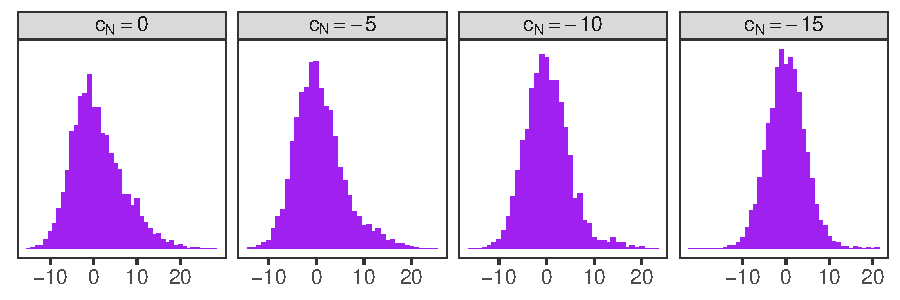
\includegraphics[width=.85\textwidth]{figures-and-tables/auxiliary/sampling_distribution.pdf}
    \caption{Sampling distribution of \(\sqrt{N} T_N - c_N\) with adaptive weighting (\(m = 1/2\)).}
    \label{fig:sampling_distribution}
\end{figure}

In the figure, we observe the following pattern: when \(c_N = 0\) (left-most panel), 
the sampling distribution of the estimator is highly skewed; 
as the magnitude of \(c_N\) increases, the distribution becomes more symmetric and eventually approaches a near-normal distribution (right-most panel). 
The shape transition of the sampling distribution from \(c_N = 0\) to \(c_N = -15\) suggests the limiting distribution of the test statistic depends on the signal strength \(c_N\). The results presented in the next section provide an exact characterization of such dependence.


\section{Theoretical results}\label{sec:weak_convergence_WIPW} 

The organization of this section is as follows. We state our main weak limit results in Section \ref{sec:weak_convergence}, followed by several remarks in Section \ref{sec:remarks_weak_convergence}. 
Section~\ref{sec:phase_transition} describes the phase transition of the limiting distribution of the test statistic across different signal strengths.
We then apply the general results to two specific adaptive experimental designs in Section \ref{sec:application}. In Section \ref{sec:bootstrap_procedure}, we propose a bootstrap procedure for hypothesis testing based on the weak limits. 

\subsection{General theory: signal-dependent weak limits}\label{sec:weak_convergence}

We first explicitly define the selection algorithm $\mathcal{S}(S_N^{(1)}(0)-S_N^{(1)}(1))$. We allow the $\mathcal{S}$ to vary across sample size $N$ so we will write $\mathcal{S}_N$ to emphasize such dependence. Suppose $\bar e(s,x)\in[0,1]$ is a sampling function for $s\in\{0,1\}$ such that $\bar e(0,x)+\bar e(1,x)=1$ for any $x\in\mathbb{R}$. Then define the sampling function
\begin{align}\label{eq:clip}
	\mathcal{S}_N(S_N^{(1)}(0) - S_N^{(1)}(1))\equiv \min\{1-l_N, \max\{l_N,\bar e(0,S_N^{(1)}(0)-S_N^{(1)}(1))\}\},
\end{align}
where $l_N$ is a positive sequence $l_N\in[0,1/2)$. 
We note that the minimum and maximum functions are mainly used for ensuring both treatments are assigned with nonzero probability in the follow-up stage when $l_N>0$. This is a reasonable assumption for many practical applications/algorithms, as it is often desirable to maintain a certain level of exploration in the follow-up stage. Such purpose includes reducing the risk of assigning treatment to the inferior group or stablizing the variance of the downstream test statistic. Such clipping strategy has been widely adopted in the literature of adaptive experiments~\citep{Zhang2020,Hadad2021}. The results in this section assume $l_N\in(0,1/2)$, i.e. strictly positive, but we will extend the results to $l_N=0$ in Section \ref{sec:extension_m_1}. We defer the discussion on the choice of $l_N$ to Remark~\ref{rmk:positivity-l-N} and \ref{rmk:early-dropping}. 

Define the extended $\mathbb{R}$ space as $\bar{\mathbb{R}}\equiv \mathbb{R}\cup \{-\infty\}$. We consider the following assumptions.
\begin{assumption}[Moment conditions]\label{assu:moment_condition}
	For any $s\in\{0,1\}$,
	\begin{align*}
		0< \inf_{N}\big(\E\left[Y_{uN}^2(s)\right]-\E\left[Y_{uN}(s)\right]^2\big)
		\leq \sup_{N}\big(\E\left[Y_{uN}^4(s)\right]\big)^{1/2}<\infty.
	\end{align*}
	For $p\in\{1,2\}, \lim_{N\rightarrow\infty}\E[Y_{uN}^{p}(s)]$ exist. Recalling $c_N\equiv \sqrt{N}(\E[Y_{uN}(0)]-\E[Y_{uN}(1)])$, we assume $\lim_{N\rightarrow\infty}c_N=c$ for $c\in[-\infty,0]$. 
\end{assumption}

\begin{assumption}[Sampling designs]\label{assu:sampling_design}
	The sampling function $\bar e(s,x)$ satisfies $\bar e(0,x)+\bar e(1,x)=1$ for any $x\in\bar{\mathbb{R}}$. Moreover, one of the following assumptions holds:
	\begin{enumerate}
		\item\textbf{Lipschitz condition:} For any $s\in\{0,1\}$, $\bar e(s,x)$ is a Lipschitz function over $x\in\bar{\mathbb{R}}$, with universal Lipschitz constant $L>0$ and $\bar e(s,-\infty)$ takes values in $\{0,1\}$;
		\item\textbf{Step-function condition:} There exist some $m_1\in\mathbb{R},K\in\mathbb{N}$ and continuous function $g:\bar{\mathbb{R}}\rightarrow\bar{\mathbb{R}}$ with $g(-\infty)=-\infty$, such that for any $s\in\{0,1\}$, 
		\begin{align*}
			\bar e(s,x)=\sum_{k=1}^K c_{k}\indicator(g(x)\in C_k)\quad\text{where}\quad c_k\in [0,1]\text{ and $C_k$ are disjoint sets},
		\end{align*}
		where $C_1=[-\infty, m_1]$ and $C_k$ are open sets for $k\geq 2$, such that $\cup_{k=2}^{K}C_k=(m_1,\infty)$.
 	\end{enumerate}
\end{assumption}

\begin{assumption}[Constant weighting]\label{assu:constant_weighting}
	Suppose $m=0$ is used and clipping rate $l_N$ (introduced in~\eqref{eq:clip}) satisfies $0<c_l<\bar l=l_N<c_u<1/2$ for any $N\in\mathbb{N}$.
\end{assumption}

\begin{assumption}[Adaptive weighting]\label{assu:adaptive_weighting}
	Suppose $m=1/2$ is used and clipping rate $l_N$ satisfies $l_N\in (0,1/2)$ for any $N\in\mathbb{N}$. Moreover, $\lim_{N\rightarrow\infty}l_N=0$ and $Nl_N\rightarrow\infty$.
\end{assumption}

We postpone the discussion on the assumptions to Section~\ref{sec:remarks_weak_convergence}. Before stating the theorem, we first describe the limiting distributions of the WIPW estimator and the test statistics $T_N,W_N$. 

\paragraph{Form of limiting distributions.}

To ease the presentation, we use $(a)_{2\times 2}$ to denote a symmetric matrix with dimension $2$, diagonal values to be $1$ and off-diagonal values to be $a$. The limiting distirbutions of both $\WIPW(s)$ and the test stiatistics $T_N$ and $W_N$, 
can be expressed as weighted sums of two dependent Gaussian vectors, $A^{(t)}\equiv (A^{(t)}(0), A^{(t)}(1))^\top$ for $t\in[2]$. Intuitively, $A^{(1)}$ corresponds to the randomness in the pilot stage 
and $A^{(2)}$ to that in the follow-up stage and is dependent on $A^{(1)}$. 
Concretely, the distributions of $A^{(t)}$ can be defined as
\begin{align*}
	A^{(1)} \sim N(\bm 0, \bm \Sigma^{(1)})\quad\text{and}\quad A^{(2)}|A^{(1)} \sim N(\bm 0, \bm \Sigma^{(2)}(A^{(1)})),
\end{align*} 
where $\bm\Sigma^{(1)}\equiv (\mathrm{Cov}^{(1)})_{2\times 2}$ and $\bm \Sigma^{(2)}(A^{(1)})\equiv (\mathrm{Cov}^{(2)}(A^{(1)}))_{2\times 2}$. The covariance $\mathrm{Cov}^{(2)}(A^{(1)})$ depends on the realization of $A^{(1)}$, and their explicit definitions can be found in Appendix~\ref{sec:explicit_form_asymptotic_distribution}.
\begin{itemize}
	\item \textbf{Weak limits of $\WIPW(s)$.} Suppose $\mathcal{W}$ stands for weighting scheme and takes values in $\{\mathcal{A},\mathcal{C}\}$, standing for adaptive and constant weighting, respectively. We use $\bar{\mathbb{W}}_{\mathcal{W}}(s)$ to denote the limiting distributions of $\WIPW(s)$ after proper centering and scaling. We will use $\overset{d}{=}$ to denote equality in distribution. Then $\bar{\mathbb{W}}_{\mathcal{W}}(s)$ can be written as
	\begin{align}\label{eq:limiting_representation_single_outcome}
		\bar{\mathbb{W}}_{\mathcal{W}}(s)\overset{d}{=}\sum_{t=1}^2 A^{(t)}(s) \bar w_{\mathcal{W}}^{(t)}(s)\quad\text{for any }s\in\{0,1\},
	\end{align} 
	where $\bar w_{\mathcal{W}}^{(t)}(s)$ varies with different weighting schemes and $\bar w_{\mathcal{W}}^{(2)}(s)$ may be dependent on $A^{(1)}$. The form of $\bar w_{\mathcal{W}}^{(t)}(s)$ can be found in Appendix~\ref{sec:explicit_form_asymptotic_distribution}.
	
	\item \textbf{Weak limits of $T_N$ and $W_N$.} Suppose $\mathcal{V}$ stands for scaling scheme and takes value in $\{\mathcal{N},\mathcal{U}\}$, standing for normalized ($W_N$) and unnormalized statistics ($T_N$), respectively. We use $\mathbb{W}_{\mathcal{V}}^{\mathcal{W}}$ to denote the limiting distributions for $T_N$ and $W_N$ after proper centering and scaling. We emphasize the dependence of $\mathbb{W}_{\mathcal{V}}^{\mathcal{W}}$ on the limiting signal strength $c$ by writing $\mathbb{W}_{\mathcal{V}}^{\mathcal{W}}=\mathbb{W}_{\mathcal{V}}^{\mathcal{W}}(c)$. Then we can write
	\begin{align}\label{eq:limiting_representation}
		\mathbb{W}_{\mathcal{V}}^{\mathcal{W}}(c)\overset{d}{=}\sum_{t=1}^2 A^{(t)}(0) w_{\mathcal{W},\mathcal{V}}^{(t)}(0) -\sum_{t=1}^2 A^{(t)}(1) w_{\mathcal{W},\mathcal{V}}^{(t)}(1)
	\end{align}
	where the weights $w_{\mathcal{W},\mathcal{V}}^{(t)}(s)$ can be written as 
	\begin{align*}
		w_{\mathcal{W},\mathcal{U}}^{(t)}(s)=\bar w_{\mathcal{W}}^{(t)}(s)\quad\text{and}\quad w_{\mathcal{W},\mathcal{N}}^{(t)}(s)=\frac{\bar w_{\mathcal{W}}^{(t)}(s) }{(\sum_{s=0}^1\sum_{t=1}^2 (\bar w_{\mathcal{W}}^{(t)}(s))^2)^{1/2}}.
	\end{align*}
	Note both $\bar w_{\mathcal{W}}^{(t)}(s)$ and $A^{(t)}(s)$ also depend on the signal strength $c$ but we omit this dependence for simplicity. 
\end{itemize} 

We summarize the definition of different limiting distributions in Table~\ref{tab:limit-dist}. 
\small
\begin{table}[!ht]
	\centering
	\caption{Summary of different limiting distributions. $\mathcal{W}$ takes values in $\{\mathcal{A},\mathcal{C}\}$.}
	\label{tab:limit-dist}
	\begin{tabular}{c|c|c|c}
	  \textbf{Test statistic} &  \textbf{Estimand} & \textbf{Weak limit} & \textbf{Limiting weight} \\
	  \hline
	  $\WIPW(s)$ & $\E[Y_{uN}(s)]$  & $\bar{\mathbb{W}}_{\mathcal{W}}$ & $\bar{w}^{(t)}_{\mathcal{W}}(s)$ \\
	  $T_N$ & $\E[Y_{uN}(0)]-\E[Y_{uN}(1)]$  & $\mathbb{W}_{\mathcal{U}}^{\mathcal{W}}$ & $w^{(t)}_{\mathcal{W},\mathcal{U}}(s)$   \\
	  $W_N$ & $\E[Y_{uN}(0)]-\E[Y_{uN}(1)]$ & $\mathbb{W}_{\mathcal{N}}^{\mathcal{W}}$ & $w^{(t)}_{\mathcal{W},\mathcal{N}}(s)$ \\
	\end{tabular}
\end{table} 
\normalsize


Now we are ready to state the main results.

\begin{theorem}[Weak convergence]\label{thm:weak_convergence_W_N}
	Suppose Assumptions \ref{assu:moment_condition}-\ref{assu:sampling_design} hold. Recall the definition $c_N\equiv \lim_{N\rightarrow\infty}\sqrt{N}(\E[Y_{uN}(0)]-\E[Y_{uN}(1)])$. The following statements hold.
	\begin{enumerate}
		\item Suppose Assumption~\ref{assu:constant_weighting} holds. Then, $\sqrt{N}(\WIPW(s)-\E[Y_{uN}(s)])$ converges weakly to $\bar{\mathbb{W}}_{\mathcal{C}}(s)$ for any $s\in\{0,1\}$. Moreover, $\sqrt{N}T_N-c_N$ and $W_N - c_N/\hat S_N$ converge weakly to $\mathbb{W}_{\mathcal{U}}^{\mathcal{C}}(c)$ and $\mathbb{W}_{\mathcal{N}}^{\mathcal{C}}(c)$, respectively.
		\item Suppose Assumption~\ref{assu:adaptive_weighting} holds. Then, $\sqrt{N}(\WIPW(s)-\E[Y_{uN}(s)])$ converges weakly to $\bar{\mathbb{W}}_{\mathcal{A}}(s)$ for any $s\in\{0,1\}$. Moreover, $\sqrt{N}T_N-c_N$ and $W_N - c_N/\hat S_N$ converge weakly to $\mathbb{W}_{\mathcal{U}}^{\mathcal{A}}(c)$ and $\mathbb{W}_{\mathcal{N}}^{\mathcal{A}}(c)$, respectively.
	\end{enumerate}
\end{theorem}

\noindent Proof of Theorem \ref{thm:weak_convergence_W_N} can be found in Appendix \ref{sec:proof_weak_convergence}. 




\subsection{Remarks on the assumptions and technical challenges}\label{sec:remarks_weak_convergence}

We present several remarks on the assumptions and technical challenges of proving Theorem~\ref{thm:weak_convergence_W_N}. 

\begin{remark}[Comments on Assumptions~\ref{assu:moment_condition}-\ref{assu:adaptive_weighting}]\label{rmk:positivity-l-N}
	
	Assumption~\ref{assu:moment_condition} is a mild regularity assumption. Assumption~\ref{assu:sampling_design} imposes mild restrictions on the sampling function,
	providing substantial flexibility for the choice of sampling function $\bar e(s,x)$ 
	(and hence the selection algorithm $\mathcal{S}$) to encode different experimental designs. To demonstrate the generality of these assumptions, we present two classes of experiments in Section~\ref{sec:application}. Now we comment on Assumption~\ref{assu:constant_weighting} and Assumption~\ref{assu:adaptive_weighting}. 
	Constant weighting, informed by Assumption \ref{assu:constant_weighting}, 
	requires the minimum sampling probability to be uniformly bounded away from $0$. In the causal inference literature, Assumption \ref{assu:constant_weighting} is known as the positivity assumption~\citep{crump2009dealing,imbens2015causal}. The adaptive weighting enables less stringent requirement on the sampling probability in the second stage encouraging further exploitation. Assumption \ref{assu:adaptive_weighting} allows minimum sampling probability in the second stage to go to zero at the rate slower than $1/N$. Similar assumption has also been adopted in \citet{Zhang2020,Hadad2021}. 
\end{remark}


\begin{remark}[Early-dropping experiments]\label{rmk:early-dropping}
	Relevant to Remark~\ref{rmk:positivity-l-N}, one kind of adaptive sampling Theorem~\ref{thm:weak_convergence_W_N} does not cover is the so-called early-dropping experiments~\citep{sampson2005drop,sill2009drop}. In these experiments, the inferior treatment will be dropped from the follow-up stage. In this case, $\mathcal{S}_N(S_N^{(1)}(0) - S_N^{(1)}(1)) $ can be $0$ or $1$. We will show in Appendix~\ref{sec:extension_m_1} that when $m=1$, we can get rid of the clipping~\eqref{eq:clip} by allowing $l_N=0$. 
\end{remark}


\begin{remark}[Technical challenges behind Theorem \ref{thm:weak_convergence_W_N}]\label{rmk:technical_challenges}
Despite the clean and nice results, proving Theorem~\ref{thm:weak_convergence_W_N} is technically challenging. Most existing weak convergence results for adaptive experiments rely on variants of the martingale central limit theorem~\citep{Zhang2020,Hadad2021}. 
However, the limiting distributions derived in Theorem~\ref{thm:weak_convergence_W_N} are generally non-normal when \( c \in (-\infty, 0] \), rendering those results inapplicable in our setting. 
Instead, we establish weak convergence from first principles using the \emph{test function approach}~\citep{Dudley_2002}. 
While inspired by the framework of \citet{che2023adaptive}, our proofs are considerably more technical due to two key challenges. 
First, unlike the test statistic adopted in \citet{che2023adaptive},\footnote{We refer the reader to Appendix~\ref{sec:inspection_Che} for more details on the test statistic analyzed in~\citet{che2023adaptive}.} our test statistics \( T_N \) and \( W_N \) have more complex dependencies on the two-stage sampled data. In particular, we must establish joint convergence for a vector of statistics that includes possibly nonlinear functionals, such as \( \mathcal{S}_N(S_N^{(1)}(0) - S_N^{(1)}(1)) \). This poses a challenge for establishing the conditional convergence of the vector of statistics contributed from the second stage, necessitating an extension of classical asymptotic tools. Notably, we introduce two new continuous mapping theorems to handle convergence under conditioning (Lemma~\ref{lem:continuous_map_varying} and \ref{lem:sufficient_condition_CMT}). Second, under adaptive weighting (Assumption~\ref{assu:adaptive_weighting}), we allow the clipping rate \( l_N \) to decay to zero relatively fast. As a result, higher-order moments of the test statistics (e.g. $T_N$ and $W_N$)  may diverge, depending on the rate at which \( l_N \) vanishes. This imposes constraints on the choice of test functions used for establishing the weak convergence and we choose to work with bounded Lipschitz test functions. As a by-product of our analysis, we establish a new version of the conditional CLT with bounded Lipschitz test functions (Lemma~\ref{lem:CLT_BL}). These new theoretical results can be applied to general setting involving dependent data and thus may be of independent interest.
\end{remark}

\subsection{Phase transition and implication on hypothesis testing}
\label{sec:phase_transition}
A key strength of our results in Theorem~\ref{thm:weak_convergence_W_N} is the weak limits can be expressed explicitly using weighted sums of two dependent Gaussian variables $A^{(t)}$ as shown in \eqref{eq:limiting_representation_single_outcome} and \eqref{eq:limiting_representation}. This allows us to understand the limiting distributions of different test statistics in a more intuitive way. We will discuss how the limiting distributions of $T_N$ and $W_N$ change as signal strength $c$ changes. Specifically, the shapes of limiting distributions are determined by the covariance $\mathrm{Cov}^{(2)}(A^{(1)})$ and random weights $w_{\mathcal{W},\mathcal{V}}^{(2)}(s)$, which are both influenced by the signal strength \( c \). Consider the following two regimes:
\begin{itemize}
	\item \textbf{Strong signal regime.} When $c=-\infty$, i.e., the absolute difference between two expected outcomes is much larger than $1/\sqrt{N}$, it can be shown that $\mathrm{Cov}^{(2)}(A^{(1)})$ and $w_{\mathcal{W},\mathcal{V}}^{(2)}(s)$ are deterministic constants. This implies that the flucutation of the first stage estimator does not affect the final limit through the limiting covariance. Therefore the final limit $\mathbb{W}_{\mathcal{V}}^{\mathcal{W}}(-\infty)$ follows a Gaussian distribution.   
	\item \textbf{Zero and weak signal regimes.} When $c\in (-\infty,0]$, the limiting distribution may no longer be a normal distribution. This is because $A^{(1)}$ will appear in the conditional distribution of $A^{(2)}|A^{(1)}$ through the limiting covariance $\mathrm{Cov}^{(2)}(A^{(1)})$. Similarly, $w_{\mathcal{W},\mathcal{V}}^{(2)}(s)$ depends on the realization of $A^{(1)}$. Therefore, when the signal is ``weak", the non-normal behavior is the ``price" one needs to pay for choosing to use the adaptive sampling scheme.
\end{itemize}

Additional insights on the non-normal limiting behaviors from double-dipping and data generating process perspectives can be found in Appendix \ref{sec:intuition_limits}. To get better intuition, 
we simulate $\mathbb{W}_{\mathcal{V}}^{\mathcal{W}}(c)$ 
with $\mathcal{V}=\mathcal{U},\mathcal{W}=\mathcal{A}$---this is the limiting distribution 
corresponding to the sampling distribution presented in Figure~\ref{fig:sampling_distribution}. 
We vary the limiting signal strength $c$ and show the simulated results in Figure \ref{fig:transition}, 
which align closely with those in Figure \ref{fig:sampling_distribution}. 
As $c$ approaches $-\infty$, i.e., as the signal gets stronger, the limiting distribution of $\mathbb{W}_{\mathcal{V}}^{\mathcal{W}}(c)$ 
approaches a normal distribution. Such phase transition, as informed by Theorem \ref{thm:smooth_transition}, is smooth with respect to signal strength $c$ under \textit{1-Wasserstein distance}, $W_1$.

\begin{figure}[!ht]
    \centering
    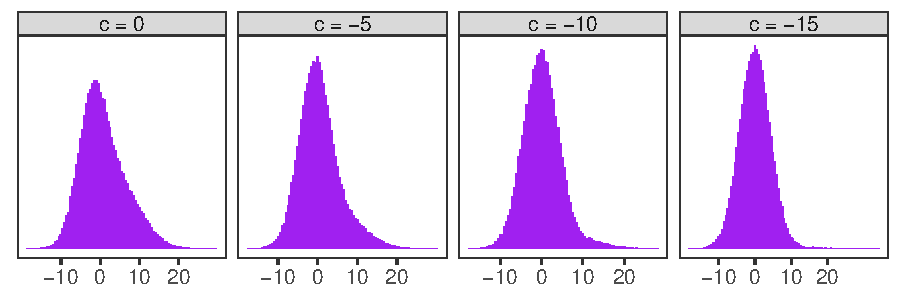
\includegraphics[width=.85\textwidth]{figures-and-tables/auxiliary/asymptotic_distribution.pdf}
    \caption{Distribution \(\mathbb{W}_{\mathcal{U}}^{\mathcal{A}}(c)\) as a function of limiting signal strength $c$.}
    \label{fig:transition}
\end{figure}

\begin{theorem}[Smooth transition of limiting distributions]\label{thm:smooth_transition}
	Suppose the assumptions of Theorem \ref{thm:weak_convergence_W_N} hold. Then for any $\mathcal{V}\in \{\mathcal{U},\mathcal{N}\}$ and $\mathcal{W}\in \{\mathcal{A},\mathcal{C}\}$, we have
	\begin{align*}
		W_1(\mathbb{W}_{\mathcal{V}}^{\mathcal{W}}(-\infty), \mathbb{W}_{\mathcal{V}}^{\mathcal{W}}(c))\rightarrow0\quad\text{as}\quad c\rightarrow-\infty.
	\end{align*}
\end{theorem}

\noindent Proof of Theorem \ref{thm:smooth_transition} can be found in Appendix \ref{sec:proof_smooth_transition}, where the definition of Wasserstein distance can also be found. Gathering these insights, we now discuss the implications of our results on hypothesis testing.

\paragraph{Implication on hypothesis testing.}

Another strength of our results lies in establishing weak convergence under minimal moment conditions, mild assumptions on the sampling functions, and broad signal strength regimes. These assumption-lean properties are not merely of theoretical interest—they carry practical significance for downstream hypothesis testing. To demonstrate the implication of our results on the hypothesis testing, consider the null hypothesis $H_{0N}:\E[Y_{uN}(0)] - \E[Y_{uN}(1)]=0$ and two alternatives within the general hypothesis $H_{1N}: \E[Y_{uN}(0)] - \E[Y_{uN}(1)] \neq 0$:
\[
H_{2N}: \E[Y_{uN}(0)] - \E[Y_{uN}(1)] = \frac{b_2}{\sqrt{N}} \quad \text{and}\quad
H_{3N}: \E[Y_{uN}(0)] - \E[Y_{uN}(1)] = \frac{b_3}{N^\beta},
\]
where $b_2, b_3 \in (-\infty, 0)$ and $\beta \in [0, 1/2)$. The contiguous alternative $H_{2N}$ corresponds to a weak signal regime, while $H_{3N}$ reflects a strong signal setting. Ideally, a test should control the Type-I error under $H_{0N}$ and achieve non-trivial power under $H_{2N}$, while attaining power approaching one under $H_{3N}$. It is also desirable for the test to remain assumption-lean with respect to the potential outcome distributions.
Our results accommodate this full range of signal strengths while maintaining minimal assumptions on the sampling functions and underlying distributions.

\paragraph{Comparison to existing literature.}
To highlight the significance of our results, we compare our results to those in related work. \citet{Zhang2020} establish asymptotic normality via stage-wise normalization under general hypotheses. Their method, however, relies on restrictive outcome distribution assumptions and yields lower power than tests based on sample means with pooled two-stage data \citep{Hirano2023}. \citet{Hadad2021} analyze the WIPW estimator for $m = 1/2$, but only in strong signal regimes (e.g., $H_{3N}$), excluding $H_{0N}$ and local alternatives. Both \citet{Zhang2020} and \citet{Hadad2021} achieve asymptotic normality under strong signals, potentially at the cost of power. \citet{Hirano2023} and \citet{adusumilli2023optimal} derive asymptotic representations for general test statistics under batched designs and contiguous alternatives $H_{2N}$, relying on classical limit-of-experiment theory by~\citet{le1972limits}. However, to apply Le Cam's theory, one must first establish the required weak convergence of certain statistics (see, for example, Theorem 2 in~\citep{Hirano2023}). Their results also assume quadratic mean differentiability (QMD) (or smooth semiparametric models), which may be restrictive in practice. A complementary line of work uses diffusion approximations with increasing batch numbers \citep{fan2021diffusion,kuang2024weak}, which differs from our two-stage setup with growing per-stage samples. Further discussion appears in Appendix~\ref{sec:inspection_literature}.

% \zr{I find this paragraph redundant given the intro. Would suggest to remove it.}


\subsection{Case study: application to different adaptive experiments}\label{sec:application}

In this section, we demonstrate the applicability of Theorem~\ref{thm:weak_convergence_W_N} to a variety of adaptive experimental designs. Specifically, we focus on two widely used paradigms: \emph{batched bandit experiments} and \emph{subgroup enrichment designs}. These designs have been studied in recent statistical and machine learning literature~\citep{russo2016simple,lin2021inference,che2024optimization,freidling2024selective}.

\paragraph{Batched bandit experiments.}

Batched bandit experiments typically employ adaptive algorithms to balance exploration and exploitation. Two commonly studied strategies are \emph{Thompson sampling} and the \emph{$\varepsilon$-greedy algorithm}. Thompson sampling is a Bayesian approach that selects actions according to their posterior probabilities of being optimal. The $\varepsilon$-greedy algorithm chooses the empirically best arm with probability $1 - \varepsilon/2$ and explores the inferior arm with probability $\varepsilon/2$ when there are two arms. We will show that Theorem~\ref{thm:weak_convergence_W_N} applies to two-batch bandit experiments employing these algorithms.

\begin{itemize}
    \item \textbf{Modified Thompson sampling:}  
    Assuming suitable prior distributions, the posterior for each expected outcome $\E[Y_{uN}(s)]$, conditional on pilot data, is (approximately) $N(S_N^{(1)}(s), 1/2)/\sqrt{N_1}$, where $N$ represents the normal distribution. This yields a sampling function:
    \begin{align*}
        \bar e(s, x) = (1 - \Phi(x)) \indicator(s = 1) + \Phi(x) \indicator(s = 0),
    \end{align*}
    which is Lipschitz continuous over $x \in \bar{\mathbb{R}}$ and satisfies the \textbf{Lipschitz condition} of Assumption~\ref{assu:sampling_design}. This algorithm has been used in~\citet{Hadad2021}. Incorporating a clipping rate $l_N$ (see Eq.~\eqref{eq:clip}), the follow-up sampling probability $\P[A_{uN}^{(2)} = 0|\mathcal{H}_{1}]$ becomes a modified Thompson sampling rule:
    \begin{align}\label{eq:modified-cliped-TS}
        \max\{l_N, \min\{1-l_N,\Phi(S_N^{(1)}(0) - S_N^{(1)}(1))\}\}.
    \end{align}

    \item \textbf{$\varepsilon$-greedy algorithm:}  
    Consider the non-smooth sampling function:
    \begin{align*}
        \bar e(s, x) = \indicator(x < 0)\indicator(s = 1) + \indicator(x \geq 0)\indicator(s = 0),
    \end{align*}
    which satisfies \textbf{Step-function condition} in Assumption~\ref{assu:sampling_design}. With clipping rate $l_N$, the follow-up sampling probability $\P[A_{uN}^{(2)} = 0|\mathcal{H}_{1}]$ corresponds to an $\varepsilon$-greedy algorithm with $\varepsilon = 2l_N$:
    \begin{align}\label{eq:eps-greedy}
        (1-l_N)\indicator(S_N^{(1)}(0) \geq S_N^{(1)}(1)) + l_N\indicator(S_N^{(1)}(0) < S_N^{(1)}(1)).
    \end{align}
\end{itemize}

\paragraph{Subgroup enrichment experiments.}

The assignment variable $A$ may indicate subgroup membership rather than treatment assignment. In this context, $Y_{uN}(0)$ and $Y_{uN}(1)$ represent outcomes for two distinct subgroups. Adaptive enrichment designs aim to identify and focus on the subgroup that benefits more from the treatment, based on interim results from pilot stage. Common strategies include enrichment based on estimated effect size or interim $p$-value~\citep{us2019adaptive,ben2024adaptive}.

\begin{itemize}
    \item \textbf{Enrichment based on effect size:}  
    The sampling function in this case is:
    \begin{align*}
        \bar e(s, x) = \indicator(x < \beta)\indicator(s = 1) + \indicator(x \geq \beta)\indicator(s = 0),
    \end{align*}
    where $\beta$ is a pre-specified threshold for the effect size.

    \item \textbf{Enrichment based on interim $p$-values:}  
    Let $\hat{\sigma}$ denote the estimated standard deviation of $S_N^{(1)}(0) - S_N^{(1)}(1)$ under the null hypothesis $H_{0N}$. Define left-sided and right-sided $p$-values as $p_l = \Phi(x / \hat{\sigma})$ and $p_r = 1 - p_l$, respectively. Given a pre-specified significance level $\alpha$, the sampling function based on interim $p$-values becomes:
    \begin{align*}
        \bar e(s, x) = \indicator(p_l < \alpha)\indicator(s = 0) + \indicator(p_r < \alpha)\indicator(s = 1) + \indicator(p_l \in [\alpha, 1 - \alpha]) \cdot 0.5,
    \end{align*}
    which introduces randomization when the interim result is inconclusive.
\end{itemize}
The follow-up sampling probabilities $\P[A_{uN}^{(2)} = 0|\mathcal{H}_{1}]$ and $\P[A_{uN}^{(2)} = 1|\mathcal{H}_{1}]$ can be similarly obtained based on these sampling functions.

\begin{remark}[Generalization of Theorem~\ref{thm:weak_convergence_W_N} to accommodate nuisance parameter]
	
	The second example of subgroup enrichment experiments falls outside the scope of Theorem~\ref{thm:weak_convergence_W_N} due to the presence of the nuisance parameter $\hat\sigma$ in the sampling mechanism. To address this, we extend our theoretical results to accommodate such nuisance parameters. This generalization is presented in Theorem~\ref{thm:weak_convergence_W_N_nuisance} in Appendix~\ref{sec:extension_nuisance}.
\end{remark}


\subsection{Asymptotically valid tests with plug-in bootstrap}\label{sec:bootstrap_procedure}


Theorem~\ref{thm:weak_convergence_W_N} characterizes the limiting behavior of WIPW test statistics, forming the basis for constructing asymptotically valid tests. 
In this section, we focus on testing whether or not the difference in means $\E[Y_{uN}(0)]-\E[Y_{uN}(1)]=0$ for demonstration. Similar results can be established for other hypotheses, for example, single outcome hypothesis $\E[Y_{uN}(s)]=0$ for some $s\in\{0,1\}$. Based on Theorem~\ref{thm:weak_convergence_W_N}, we can define the following asymptotically valid tests: for any $\mathcal{W} \in \{\mathcal{A}, \mathcal{C}\}$,
\begin{align}\label{eq:four_tests}
    \phi_{\mathcal{U}}^{\mathcal{W}} \equiv \indicator \big(\sqrt{N}T_N \geq \mathbb{Q}_{1-\alpha}(\mathbb{W}_{\mathcal{U}}^{\mathcal{W}}(0))\big)\quad\text{and}\quad\phi_{\mathcal{N}}^{\mathcal{W}} \equiv \indicator \big(W_N \geq \mathbb{Q}_{1-\alpha}(\mathbb{W}_{\mathcal{N}}^{\mathcal{W}}(0))\big).
\end{align}
The critical values \(\mathbb{Q}_{1-\alpha}(\mathbb{W}_{\mathcal{V}}^{\mathcal{W}}(0))\) are the \((1-\alpha)\)-th quantiles of the limiting distribution \(\mathbb{W}_{\mathcal{V}}^{\mathcal{W}}(0)\) defined in Theorem~\ref{thm:weak_convergence_W_N}. However, tests in~\eqref{eq:four_tests} cannot be implemented in practice for two reasons. First, the asymptotic distributions \(\mathbb{W}_{\mathcal{V}}^{\mathcal{W}}(0)\) are generally non-normal (see also the left-most subplot in Figure \ref{fig:transition}). Second, the limiting distribution involves unknown nuisance parameters, which have to be estimated using observed data. In this section, we propose a bootstrap procedure to address these challenges and construct valid tests, which can be implemented in practice.

\paragraph{A fast bootstrap procedure.} 

Note that the expression of limiting distribution in~\eqref{eq:limiting_representation} is a weighted sum of two dependent Gaussian variables. Motivated by such observation, we propose a plug-in bootstrap procedure to obtain the quantile information $\mathbb{Q}_{1-\alpha}(\mathbb{W}_{\mathcal{V}}^{\mathcal{W}}(0))$. For the ease of presentation, we will omit the definition of nuisance estimators and present a simplified algorithm in Algorithm~\ref{alg:sampling_weighting_simplified}. The complete bootstrap procedure with the estimators of nuisance parameters can be found in Appendix~\ref{sec:bootstrap_algorithm}.
\small
\begin{algorithm}[!ht]
    \SetAlgoNlRelativeSize{0} 

    \nonl \textbf{Input:} Outcome mean estimators $\hat\E[Y_{uN}(s)]$ and $\hat\E[Y_{uN}^2(s)]$; estimators $\hat{\mathrm{Cov}}^{(1)}$ and $\hat{\mathrm{Cov}}^{(2)}(\cdot)$; weighting and scaling schemes $\mathcal{W}\in\{\mathcal{A},\mathcal{C}\}$ and $\mathcal{V}\in\{\mathcal{U},\mathcal{N}\}$; sampling funciton $\bar e(s,\cdot)$; clipping rate $l_N$. \\

    \textbf{First stage sampling:} Compute $\tilde{A}^{(1,b)} = (\hat{\bm{\Sigma}}^{(1)})^{1/2} S_1^{(b)}$, $S_1^{(b)} \sim N(0, \bm{I}_2)$, with $\hat{\bm{\Sigma}}^{(1)} = (\hat{\mathrm{Cov}}^{(1)})_{2 \times 2}$.
    
    \textbf{Second stage sampling:} Compute $\tilde{A}^{(2,b)} = (\hat{\bm{\Sigma}}^{(2,b)})^{1/2} S_2^{(b)}$, $S_2^{(b)} \sim N(0, \bm{I}_2)$, with $\hat{\bm{\Sigma}}^{(2,b)} = (\hat{\mathrm{Cov}}^{(2)}(\tilde{A}^{(1,b)}))_{2 \times 2}$.

    \textbf{Weighting procedure:} Compute estimates $\hat{w}_{\mathcal{W},\mathcal{V}}^{(t,b)}(s)$ for $w_{\mathcal{W},\mathcal{V}}^{(t,b)}(s)$ with $\tilde{A}^{(t,b)}$, $ \hat\E[Y_{uN}(s)],\hat\E[Y_{uN}^2(s)],\bar e(s,\cdot)$ and $l_N$. Defining $(\tilde{A}^{(t,b)}(0),\tilde{A}^{(t,b)}(1))^{\top}\equiv\tilde{A}^{(t,b)}$, generate bootstrap sample
	\small
    \begin{align*}
		\mathcal{D}_{\mathcal{W},\mathcal{V}}^{(b)} = \sum_{t=1}^2 \hat{w}_{\mathcal{W},\mathcal{V}}^{(t,b)}(0) \tilde{A}^{(t,b)}(0) - \sum_{t=1}^2 \hat{w}_{\mathcal{W},\mathcal{V}}^{(t,b)}(1)\tilde{A}^{(t,b)}(1).
	\end{align*}
	\normalsize

    \textbf{Repeated sampling:} Repeat steps 1-3 to get $B$ bootstrap resamples.

    \nonl \textbf{Output:} Bootstrap sample $\{\mathcal{D}_{\mathcal{W},\mathcal{V}}^{(b)}:b\in[B]\}$.
    \caption{Simplified two-stage sampling and weighting procedure}
    \label{alg:sampling_weighting_simplified}
\end{algorithm}
\normalsize

We make the following remarks regarding the proposed bootstrap procedure.

\begin{remark}[Computational efficiency]
	The computational cost of generating a boostrap sample in Algorithm~\ref{alg:sampling_weighting_simplified} is $O(1)$, leading to a total cost of $O(B)$ 
	for the whole procedure. This is much more efficient than the general nonparametric bootstrap
	even with linear computation cost for computing each test statistic, which takes $O(BN)$ 
	to generate $B$ samples.
\end{remark}

\begin{remark}[A nonparametric simulation-based approach]
	Notably, Algorithm~\ref{alg:sampling_weighting_simplified} mimics a two-stage asymptotic experiment to approximate the limiting distribution of the test statistic in~\eqref{eq:limiting_representation}. From this perspective, our bootstrap approach is conceptually aligned with the simulation-based methods that leverage asymptotic representation results, as proposed in \citet{Hirano2023}. Our method is nonparametric and free of distributional assumptions, thereby enabling more robust and widely applicable inference.
\end{remark}
\paragraph{Asymptotic valid tests with plug-in bootstrap.}

Based on Algorithm~\ref{alg:sampling_weighting_simplified}, we construct the plug-in bootstrap tests using the bootstrap samples $\mathcal{D}_{\mathcal{W},\mathcal{V}}^{(b)}$. Denote the $\sigma$-algebra generated by the observed data as $\mathcal{G}_N\equiv \sigma(\mathcal{H}_1\cup\mathcal{H}_2)$. Suppose $\mathcal{D}_{\mathcal{W},\mathcal{V}}\overset{d}{=}\mathcal{D}_{\mathcal{W},\mathcal{V}}^{(b)}$, conditional on $\mathcal{G}_N$. Then for $\mathcal{W} \in \{\mathcal{A}, \mathcal{C}\}$, define
\[
\hat{\phi}_{\mathcal{U}}^{\mathcal{W}} \equiv \indicator\big(\sqrt{N} T_N > \mathbb{Q}_{1 - \alpha}(\mathcal{D}_{\mathcal{W}, \mathcal{U}}\mid \mathcal{G}_N)\big)\quad\text{and}\quad 
\hat{\phi}_{\mathcal{N}}^{\mathcal{W}} \equiv \indicator\big(W_N > \mathbb{Q}_{1 - \alpha}(\mathcal{D}_{\mathcal{W},\mathcal{N}}\mid \mathcal{G}_N)\big).
\]
The following theorem shows the validity of the plug-in bootstrap procedure and corresponding bootstrap tests. 

\begin{theorem}[Validity of plug-in bootstrap and tests $\hat \phi_{\mathcal{V}}^{\mathcal{W}}$]\label{thm:bootstrap}
	Suppose Assumption \ref{assu:moment_condition}-\ref{assu:sampling_design} hold. Then, the following statements hold.
	\begin{enumerate}
		\item Suppose Assumption \ref{assu:constant_weighting} holds, we have for $\mathcal{V}\in \{\mathcal{U},\mathcal{N}\}$,
		\begin{align*}
			\sup_{x\in\mathbb{R}}\left|\P\left[\mathcal{D}_{\mathcal{C},\mathcal{V}}\leq x|\mathcal{G}_N\right]-\P[\mathbb{W}_\mathcal{V}^{\mathcal{C}}(0)\leq x]\right|\convp 0\quad\text{and}\quad\lim_{N\rightarrow\infty}\E_{H_{0N}}[\hat \phi_{\mathcal{V}}^{\mathcal{C}}]=\alpha;
		\end{align*}
		\item Suppose Assumption \ref{assu:adaptive_weighting} holds, we have for $\mathcal{V}\in \{\mathcal{U},\mathcal{N}\}$,
		\begin{align*}
			\sup_{x\in\mathbb{R}}\left|\P\left[\mathcal{D}_{\mathcal{A},\mathcal{V}}\leq x|\mathcal{G}_N\right]-\P[\mathbb{W}_\mathcal{V}^{\mathcal{A}}(0)\leq x]\right|\convp 0\quad\text{and}\quad\lim_{N\rightarrow\infty}\E_{H_{0N}}[\hat \phi_{\mathcal{V}}^{\mathcal{A}}]=\alpha.
		\end{align*}
	\end{enumerate}
\end{theorem}

The proof of Theorem~\ref{thm:bootstrap} can be found in Appendix~\ref{sec:proof_bootstrap}. 
There is an implicit assumption we make behind Theorem \ref{thm:bootstrap}, 
which is the knowledge of the sampling function $\bar e(s,\cdot)$ and $l_N$. In practice, this assumption is reasonable since the selection algorithm or the experimental protocol is usually pre-specified before the data is collected and thus is at the hand of the experiment designer. In fact, this is the case in many empirical studies including \citet{collins2007multiphase,li2010contextual,offer2021adaptive,hannah_a_jin_2023_8192805}.



\section{Finite-sample evaluation}\label{sec:finite-sample}

In this section, we conduct extensive numerical simulations and a semi-synthetic data analysis to investigate the finite-sample performance of the tests studied in the previous section. 
In particular, we include all four bootstrap tests with two scaling and two weighting schemes proposed in Section~\ref{sec:bootstrap_procedure}. 
As a benchmark, we also include the IPW test statistic based on sample splitting, which only uses the data from follow-up stage for inference; 
the comparison demonstrates the benefit of using data from both stages. The significance level is taken to be $0.05$ throughout this section.

\subsection{Numerical simulation}\label{sec:simulation}

\paragraph{Data generation procedure.} We consider two potential outcome distributions: 
\begin{enumerate}
	\item \textbf{Binary outcome:} $Y_{uN}(0)\sim \mathrm{Bern}(\theta+0.5),\ Y_{uN}(1)\sim \mathrm{Bern}(0.5)$;
	\item \textbf{Continuous outcome:} $Y_{uN}(0)\sim N(\theta,1),\ Y_{uN}(1)\sim N(0,0.25)$.
\end{enumerate}
%We consider the two-stage setup. 
In the pilot stage, we employ the equal sampling in the pilot stage $e(1)=0.5$, which mimics the common practice in real world when there is no prior information which treatment is better. Insipired by batched bandit setup, we consider two selection algorithms: the modified version of Thompson sampling~\eqref{eq:modified-cliped-TS} and $\varepsilon$-greedy algorithm~\eqref{eq:eps-greedy}, both with clipping $l_N=\varepsilon/2$. In the second stage, we sample two treatments based on the results of these selection algorithm. The task is to test if the treatment effect is significantly different from $0$, i.e. $\theta=\E[Y_{uN}(0)]-\E[Y_{uN}(1)]=0$, or not.

\paragraph{Parameter setup.} In both selection algorithms, we set $\varepsilon \in\{ 0.1, 0.2, 0.4\}$. The signal strength $\theta$ ranges from $-0.2$ to $0.2$ with equal sapce $0.05$, with $\theta=0$ corresponding to the null hypothesis. The number of total samples $N=1000$ and each batch has the same sample size $N_1=N_2=500$. 



\begin{figure}[!ht]
	\centering
	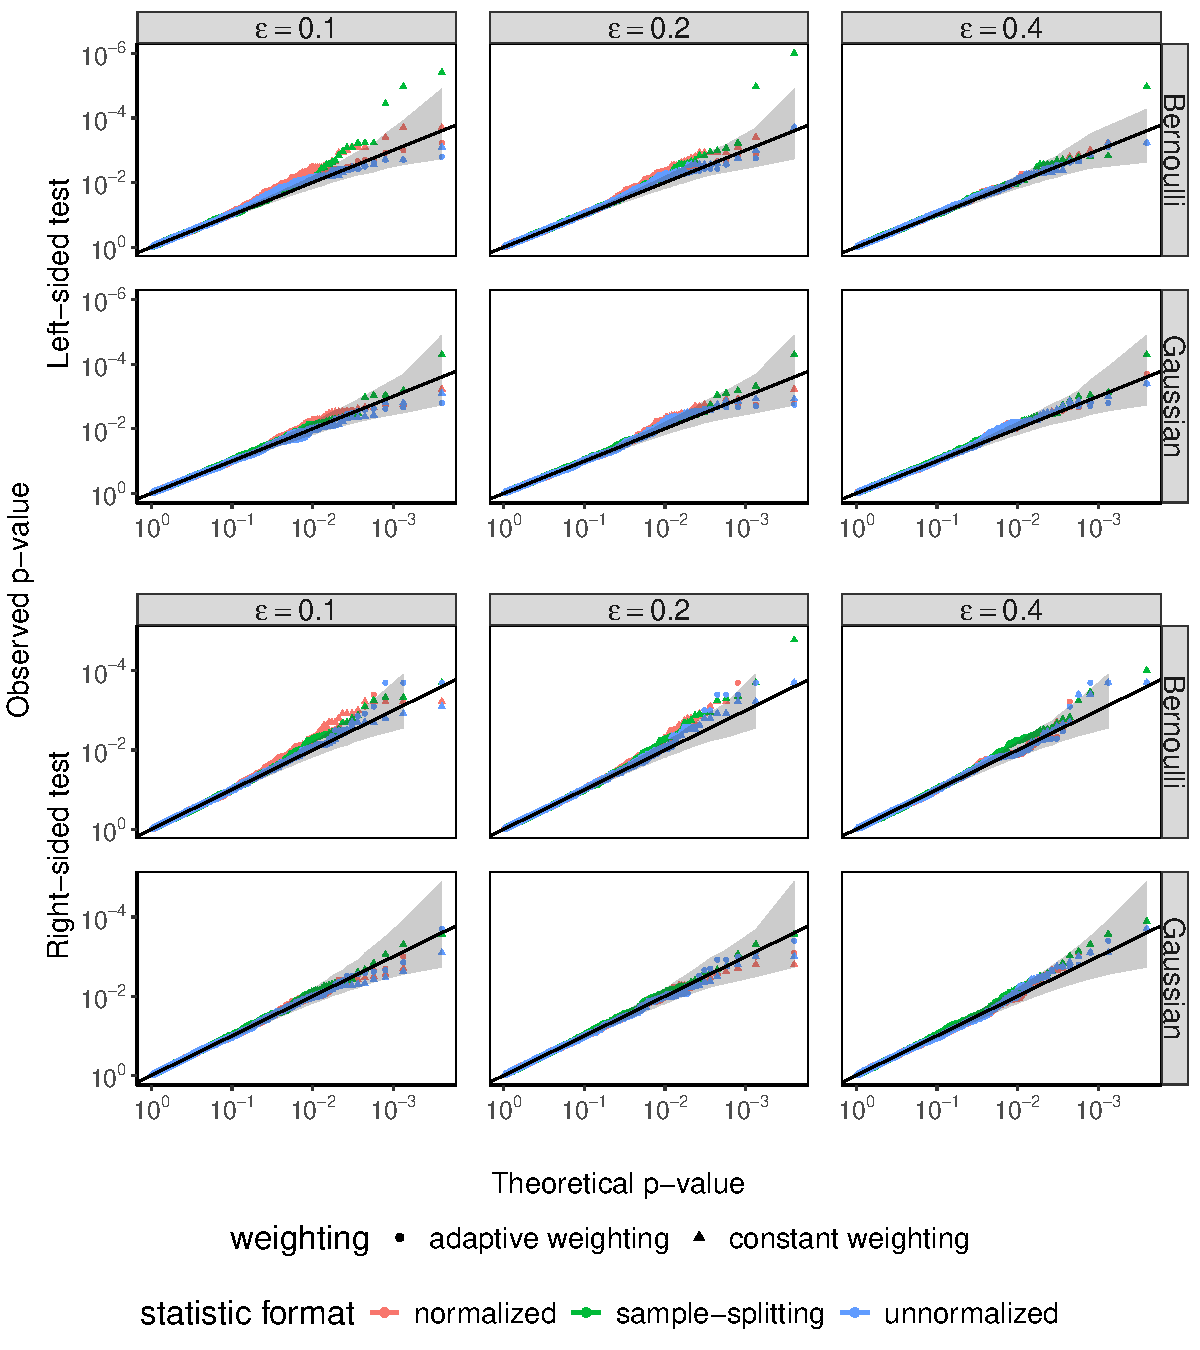
\includegraphics[width=0.95\textwidth]{figures-and-tables/simulation/thompson_qq_plot.pdf}

	\caption{QQ plots for the $5$ tests under different signal strengths. The simulation is repeated for $2000$ times. The number of bootstrap used in each test is $5000$.}
	\label{fig:simulation-qq-plot-thompson}
\end{figure}

\begin{figure}[!ht]
	\centering
	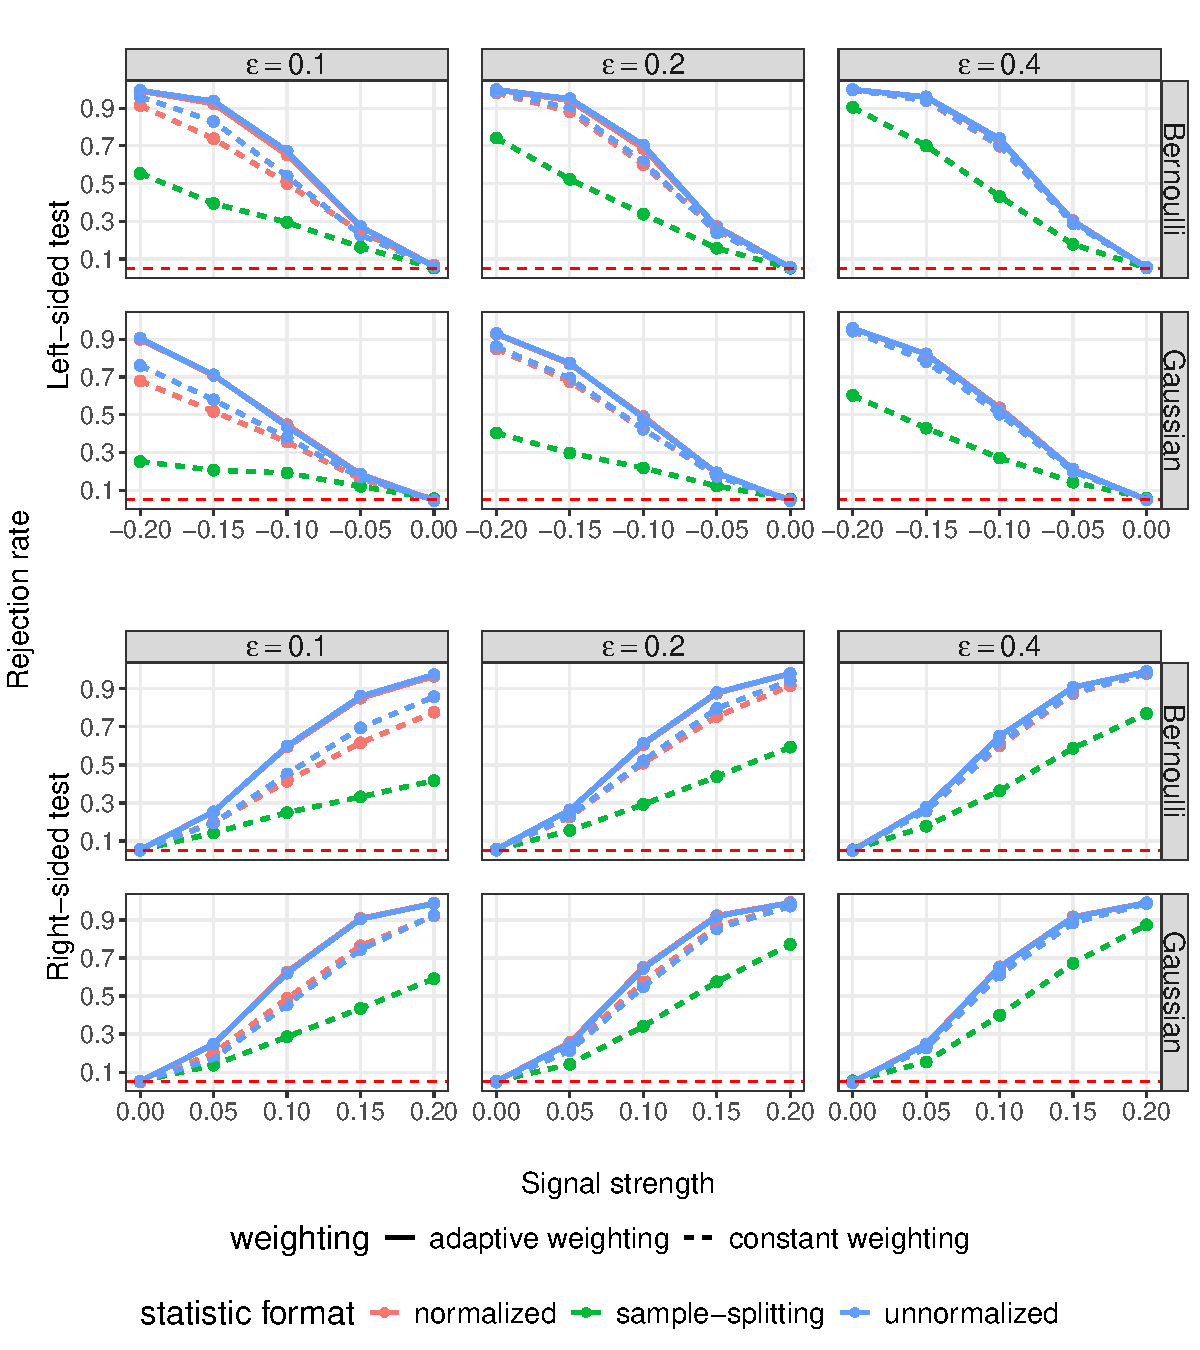
\includegraphics[width=0.95\textwidth]{figures-and-tables/simulation/thompson_rejection_plot.pdf}

	\caption{Rejection rate for the $5$ tests under different signal strength. The simulation is repeated for $2000$ times. The number of bootstrap used in each test is $5000$.}
	\label{fig:simulation-rejection-plot-thompson}
\end{figure}


\paragraph{Results analysis and interpretation.}

For the ease of presentation, we select the representative results with Thompson sampling being the selection algorithm. For additional simulation results with $\varepsilon$-greedy algorithm, we refer the readers to Appendix \ref{sec:additional_simulation}. The calibration results are summarized as QQ plots in Figure \ref{fig:simulation-qq-plot-thompson} and the power results are summarized in Figure \ref{fig:simulation-rejection-plot-thompson}. From Figure \ref{fig:simulation-qq-plot-thompson}, we observe that all the tests can produce relatively well-calibrated $p$-values. This validates the bootstrap procedure proposed in Algorithm \ref{alg:sampling_weighting_simplified}. For power comparison, it is unsurprising to see that our approach using pooled two-stage data can improve power over sample splitting. Moreover, we make the following intriguing obsevations:
\begin{enumerate} 
	\item \textbf{Tests based on adaptive weighting are more powerful.} Tests with adaptive weighting (solid lines) show substantial power improvement compared to tests with constant weighting, no matter which scaling is used. The improvement is especially pronounced when $\varepsilon$ is small. This is mainly because when constant weighting is used, WIPW estimator boils down to the usual IPW estimator. It is well-known that IPW estimator is highly variable when the downsampling on one arm in the second stage is substantial due to small $\varepsilon$.
	\item \textbf{Tests based on adaptive weighting are robust to $\varepsilon$.} Relevant to the previous point, tests based on constant weighting (including sample splitting) are more sensitive to the $\varepsilon$ in the selection algorithm. The adaptive weighting scheme, on the other hand, is more robust to the choice of $\varepsilon$. This is because the adaptive weighting scheme can adjust the weights based on the observed data, making it less sensitive to $\varepsilon$. In experimental practice, employing adaptive weighting scheme for inference enables more aggressive exploitation strategies in sampling.
	\item \textbf{Normalization influences each test in distinct ways.} Unlike the randomized controlled experiments, the normalization can make a difference in the power of the tests, even asymptotically (see Theorem \ref{thm:weak_convergence_W_N} on results with $T_N$ and $W_N$). We can observe a power gain when using unnormalized test with constant weighting (see plots in first column of Figure \ref{fig:simulation-rejection-plot-thompson}). However, from a theoretical standpoint, it remains unclear whether the unnormalized test exhibits greater power under more general data generating processes. 
	\item \textbf{Power curve depends on the sideness of the test.} We observe that the power performance differs between left-sided and right-sided tests. Under Bernoulli sampling, the left-sided test tends to reject more often across all methods, even when the absolute signal magnitudes are the same. In contrast, under Gaussian sampling, the right-sided test exhibits greater power. These observations highlight the potential need for side-dependent experimental design strategies.
\end{enumerate}


\subsection{Semi-synthetic data analysis}\label{sec:semi-sythetic-data}

To further investigate the performance of different tests on real data,  
we conduct a semi-synthetic data analysis designed to better mimic real-world settings.  
The data is derived from the Systolic Blood Pressure Intervention Trial (SPRINT) \citep{ambrosius2014design}. This is a randomized controlled trial and evaluates whether a new treatment program for lowering systolic blood pressure reduces the risk of cardiovascular disease (CVD). The population is divided into treatment (new treatment) and control (placebo) group and primary clinical outcome is the occurrence of a major CVD event.  
We generate the semi-synthetic data, apply the tests, and evaluate their performance through the following procedures.

\begin{enumerate}
    \item \textbf{Permute data to break the dependence.}  
    We first permute the outcomes within the whole population, generating $B = 500$ permuted samples.  
    This permutation effectively removes any treatment effect, ensuring that the treatment and control groups have the same expected outcome level.
    
    \item \textbf{Add signal back to the data.}  
    For these $500$ permuted samples, we manually introduce a treatment effect by increasing the mean outcome (i.e. the major CVD event occurrence) in the control group, 
    since the new treatment is intended to reduce the risk of CVD. Let $N_c^0$ denote the total number of control-group participants who did not experience a CVD event. We set $n_0$ of these zero outcomes to $1$, where $n_0 \sim \mathrm{Bin}(N_c^0,\eta)$. The added signal $\eta$ varies within the set $\{0, 0.015, 0.03, 0.045, 0.06\}$.
    
    \item \textbf{Adaptively sample the data to maximize welfare.}  
    For each permuted sample, we simulate adaptive sampling. We first draw $N_1 = 1000$ random samples. Because the new treatment could be beneficial for the patients, we apply the $\varepsilon$-greedy algorithm~\eqref{eq:eps-greedy} to collect additional $N_2 = 1000$ samples in the second stage, encouraging assignment of new treatment. We vary $\varepsilon \in \{0.1, 0.2, 0.4\}$.
    
    \item \textbf{Evaluate Type-I error control and power.}  
    We apply the five tests introduced in Section~\ref{sec:simulation} to the synthetically generated data. We consider the right-sided test to see if the CVD event rate in the control group ($\E[Y_{uN}(0)]$) is higher than that in the treatment group ($\E[Y_{uN}(1)]$). We evaluate Type-I error control before introducing signal and statistical power after introducing the signal.
\end{enumerate}
\begin{figure}[!ht]
	\centering  
	\begin{subfigure}{\textwidth}
	  \centering
	  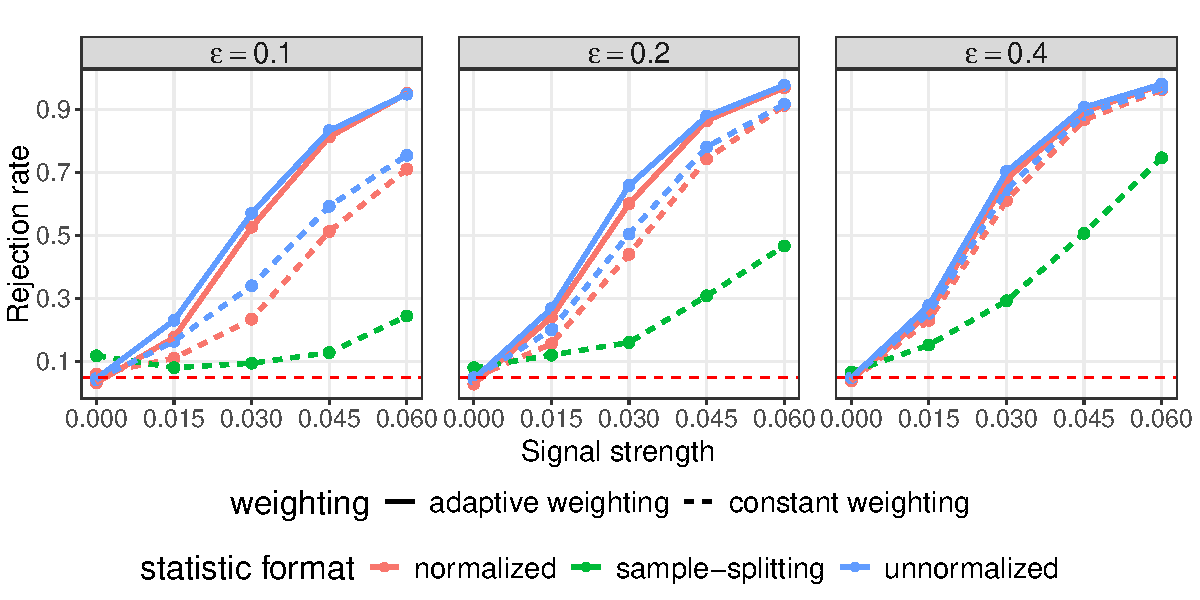
\includegraphics[width=0.9\textwidth]{figures-and-tables/realdata/rejection_plot.pdf}
	\end{subfigure}
	\caption{Type-I error and power for the five tests under semi-synthetic data. }
	\label{fig:semi-synthetic-data}
\end{figure}

The results are presented in Figure \ref{fig:semi-synthetic-data}. Perhaps a bit surprisingly, we observe that the test based on sample splitting suffers from Type-I error inflation in the absence of signal. This issue is primarily due to the sparsity of the outcome: the average rate of CVD occurrence is less than $0.1$. Such sparsity may prevent the central limit theorem from taking effect, posing a particular challenge for sample splitting, which uses only half of the data. We also find that the choice of $\varepsilon$ influences calibration performance: in the $\varepsilon$-greedy algorithm, a smaller $\varepsilon$ results in a smaller effective sample size in the second stage. Consequently, Type-I error inflation in the sample-splitting method is mitigated as $\varepsilon$ increases. In contrast, our methods control Type-I error well and $\varepsilon$ has a much smaller effect on these tests, which combine data from both stages and thus have higher effective sample size. A further investigation of calibration performance is provided in Appendix~\ref{sec:additional_semi_synthetic}. Regarding power, the benefit of adaptive sampling remains evident compared to the sample-splitting approach. Among all 4 tests proposed in this paper, the unnormalized test exhibits slightly higher power than the normalized test, although the difference is modest.

\section{Conclusion and discussion}\label{sec:discussion}

In this paper, we establish a set of general and assumption-lean weak convergence results for the WIPW estimator under a two-stage adaptive sampling scheme. These results are largely agnostic to any specific outcome distribution, allowing for broad applicability across a wide range of potential outcomes. Moreover, they accommodate a broad spectrum of signal strengths, making them especially useful for downstream hypothesis testing. To facilitate asymptotically valid tests based on these weak convergence results, we propose a plug-in bootstrap procedure that is highly scalable. Finally, we validate our theoretical claims through extensive numerical simulations and a semi-synthetic data analysis, illustrating strong finite-sample performance of the proposed tests. 

There are two directions that can be directly pursued with the results and techniques developed in this paper.
\begin{itemize}
	\item \textbf{Experimental design:} In practice, designing the adaptive experiments often requires balancing statistical goals (e.g., power) with non-statistical considerations (e.g., regret, welfare) under budget constraints. Investigating the optimal design of adaptive experiments that trade off these competing objectives is a compelling direction for future study. See, for instance, recent work on adaptive experimental design in \citet{che2023adaptive,liang2023experimental,simchi2023multi,li2024double}. Our results on limiting distributions and proposed bootstrap procedure simplify power calculations, which in turn can inform the design of adaptive experiments. 
	
	\item \textbf{Covariate adjustment:} In randomized controlled experiments, it is well established that appropriately adjusting for predictive covariates can improve the efficiency of statistical inference and increase the power of hypothesis testing \citep{lin2013agnostic}. It would be valuable to explore how such covariate adjustments can be incorporated into the analysis of data collected from adaptive experiments, and how they may enhance the efficiency of the proposed tests. These investigations require the study of asymptotic efficiency of different tests and the techniques developed in this paper may provide a useful starting point for exploring this line of research. In Appendix \ref{sec:extension_augmentation}, we present preliminary results on augmenting the WIPW test statistics.
\end{itemize}

There are several limitations in our current work that point to promising directions for future research. We summarize them below.

\begin{itemize}
	
	\item \textbf{Beyond two-stage experiments:} In this paper, we focus on a two-stage adaptive sampling scheme. However, other adaptive designs exist that fall outside this framework, such as fully adaptive sampling schemes \citep{lai1985asymptotically}, early-stopping experiments~\citep{sampson2005drop,sill2009drop} and experiments with adaptive stopping rules \citep{bauer1994evaluation}. We have sketched the extension of our results to the latter two classes of adaptive sampling strategies in Section~\ref{sec:extension_m_1} and \ref{sec:extension_stopping_time}, respectively. For the fully adaptive sampling schemes, we refer the readers to \citet{khamaru2024inference,han2024ucb,ren2024lai} for recent works on this topic. 
	
	\item \textbf{Statistical optimality:} The statistical optimality of the proposed tests remains an open question. We investigate this question by  providing preliminary comparisons of power between the $m = 1/2$ and $m = 1$ weightings in Appendix~\ref{sec:power-comparison}. It would be interesting to study semiparametrically efficient test statistic for testing the hypothesis $H_{0N}:\E[Y_{uN}(0)] = \E[Y_{uN}(1)]$ under suitable sub-classes of the general nonparametric data generating process. Although \citet{Hirano2023,adusumilli2023optimal} derive power functions via the Neyman-Pearson lemma, devising practical tests that attain the stated optimal power remains an open problem. Furthermore, for more complex scenarios—such as composite alternatives—the corresponding optimality theory remains undeveloped. 
\end{itemize}

\subsection*{Acknowledgments}
We thank Keisuke Hirano and Stefan Wager for helpful discussions and suggestions. Z.R. is supported by the National Science Foundation (NSF) under grant DMS-2413135 and 
Wharton Analytics.


\printbibliography

\clearpage

\appendix


\addtocontents{toc}{\protect\setcounter{tocdepth}{2}}
\renewcommand{\contentsname}{Appendix}


\tableofcontents

\paragraph{Notation.}
Throughout the appendix, we will use $(a,b)$ to denote a column vector for $a\in\mathbb{R}^{k},b\in \mathbb{R}^{d}$ when there is no ambiguity. In other words, we use $(a,b)$ to represent $(a^\top,b^\top)^\top$ and we omit the transpose operator for ease of presentation. Thus when we write $f(x,y)$ for $x,y$ as vectors, we will use $f(x,y)$ to denote the function $f((x^\top,y^\top)^\top)$. We use $\mathcal{C}^2(\mathcal{X})$ as the class of functions that are twice continuously differentiable on the domain $\mathcal{X}$. We use $\bm 0_k$ to denote a $k$-dimension vector with each dimension being $0$ and $\bm I_k$ to denote the identify matrix with dimension $k$. We will drop the subscript $k$ if there is no ambiguity. We use $\mathbb{N}_{+}$ to denote the positive natural number. We denote $\partial C_k$ as the boundary set of $C_k$. We denote $\nabla g$ as the gradient of a differentiable function $g$. We denote $a_N\lesssim b_N$ if there exists $c>0$ such that $|a_N/b_N|\leq c$ for large enough $N$. 
\textit{Without loss of generality, we will only prove the results in all the main text when $q_t=1/2$ for $t\in[2]$, i.e., two batches have the same sample size.} 


\section{Explicit form of the asymptotic distributions}\label{sec:explicit_form_asymptotic_distribution}


We define the limiting probabilities 
\small
\begin{align}\label{eq:limiting_probabilities}
	H^{(1)}(s)\equiv \lim_{N\rightarrow\infty}\bar e_N(s,\mathcal{H}_0)=e(s),~
	H^{(2)}(s)\equiv \max\Big\{\lim_{N\rightarrow\infty}l_N, \bar e(s,S((A^{(1)},V^{(1)}),c))\Big\}.
\end{align}
\normalsize
The function $S(x,y):\mathbb{R}^{4}\times \bar{\mathbb{R}}\rightarrow\bar{\mathbb{R}}$ is defined as 
\begin{align}\label{eq:def_h_function}
	S(x,y)\equiv x_1\cdot x_3^{1/2}/e^{1/2}(0)-x_2\cdot x_4^{1/2}/e^{1/2}(1)+y/\sqrt{2},
\end{align}
where $x=(x_1,x_2,x_3,x_4)^\top\in\mathbb{R}^4$ and $y\in \bar{\mathbb{R}}$.  Also define the scaled asymptotic variance as 
\begin{align}\label{eq:limiting_variance}
	V^{(t)}(s) \equiv \lim_{N\rightarrow\infty}\E[Y_{uN}^2(s)]-H^{(t)}(s)(\lim_{N\rightarrow\infty}\E[Y_{uN}(s)])^2,
\end{align}
and denote $R^{(t)}(s)\equiv (H^{(t)}(s)/V^{(t)}(s))^{1/2}$. Now we define the covariances for $A^{(t)}$ as follows.

\paragraph{Distribution of $A^{(1)}$.}

The covariance $\mathrm{Cov}^{(1)}$ can be defined as
\begin{align}\label{eq:covariance_A_1}
	\mathrm{Cov}^{(1)}\equiv - \left(\frac{H^{(1)}(0)H^{(1)}(1)}{V^{(1)}(0)V^{(1)}(1)}\right)^{1/2}\lim_{N\rightarrow\infty}\left(\E[Y_{uN}(0)]
	\E[Y_{uN}(1)]\right).
\end{align}


\paragraph{Distribution of $A^{(2)}$.}


The asymptotic covariance structure $\mathrm{Cov}^{(2)}(A^{(1)})$ can be written as
\begin{align}\label{eq:covariance_A_2}
	\mathrm{Cov}^{(2)}(A^{(1)})\equiv - \left(\frac{H^{(2)}(0)H^{(2)}(1)}{V^{(2)}(0)V^{(2)}(1)}\right)^{1/2}\lim_{N\rightarrow\infty}\left(\E[Y_{uN}(0)]
	\E[Y_{uN}(1)]\right).
\end{align}
Now we define the weights $\bar w_{\mathcal{W}}^{(t)}(s)$. To this end, we need the following auxiliary random variables,
\begin{align*}
	M_{\mathcal{A}}^{(t)}(s)\equiv q_t\Big(\frac{(H^{(t)}(s))^{1/2}}{\sum_{t=1}^2 q_t (H^{(t)}(s))^{1/2}}\Big)^2\quad\text{and}\quad M_{\mathcal{C}}^{(t)}(s)\equiv q_t.
\end{align*}
Then we can write the weights as 
\begin{align*}
	\bar w_{\mathcal{W}}^{(t)}(s)=\big(M_{\mathcal{W}}^{(t)}(s)/(R^{(t)}(s))^2\big)^{1/2}\quad\text{for any }s\in\{0,1\}\quad\text{and}\quad \mathcal{W}\in\{\mathcal{A},\mathcal{C}\}.
\end{align*}



\section{Simulation detail for Figures~\ref{fig:sampling_distribution}-\ref{fig:transition}}\label{sec:illustration_simulation}

We present the simulation details for Figure \ref{fig:sampling_distribution} and Figure \ref{fig:transition} respectively. 

\paragraph{Figure \ref{fig:sampling_distribution}.}
To generate Figure \ref{fig:sampling_distribution}, we consider the following potential outcome model: 
\begin{align}\label{eq:simulation-model}
	Y_{uN}(0)\sim N(0,1),\ Y_{uN}(1)\sim N(-c_N/\sqrt{N},9),\ c_N\in\{0,-5,-10,-15\}.
\end{align}
We set the sample size $N=1000$ and the batch size $N_1=N_2=500$. 
The initial sampling $e(0)=e(1)=0.5$ and $\varepsilon$-greedy algorithm is used with $\varepsilon=0.05$. The simulations are repeated $5000$ times.

\paragraph{Figure \ref{fig:transition}.}

We use the covariance structure~\eqref{eq:covariance_A_1} and \eqref{eq:covariance_A_2}, to simulate the limiting distribution~\eqref{eq:limiting_representation}. We set $q_t=1/2$ and assume the knowledge of the first and second moments $\E[Y_{uN}(s)],\E[Y_{uN}^2(s)]$ from model~\eqref{eq:simulation-model}. Set the limiting signal strength $c\in \{0,-5,-10,-15\}$. The simulations are repeated $100,000$ times.


\section{Details of bootstrap algorithm in Section~\ref{sec:bootstrap_procedure}}\label{sec:bootstrap_algorithm}


We begin by estimating the necessary nuisance parameters for the bootstrap in Appendix~\ref{sec:bootstrap_nuisance} and then provide the detailed bootstrap algorithm in Appendix~\ref{sec:bootstrap_algorithm_detail}.

\subsection{Nuisance parameter estimation}\label{sec:bootstrap_nuisance}

Analogous to the estimator $\hat{\E}[Y_{uN}(s)]$ in \eqref{eq:WIPW_estimator}, we estimate $\E[Y_{uN}^2(s)]$ using:
\small
\begin{align}\label{eq:WIPWS_estimator}
	\WIPWS(s) \equiv \sum_{t=1}^2 \frac{N_th_{N}^{(t)}(s)}{\sum_{t=1}^2 N_t h_{N}^{(t)}(s)} \cdot \frac{1}{N_t} \sum_{u=1}^{N_t} \tilde{\Lambda}_{uN}^{(t)}(s)\quad \text{and}\quad
	\tilde{\Lambda}_{uN}^{(t)}(s) \equiv \frac{\indicator(A_{uN}^{(t)}=s)(Y_{uN}^{(t)})^2}{\P[A_{uN}^{(t)}=s|\mathcal{H}_{t-1}]}.
\end{align}
\normalsize
Using these, we estimate the first-stage variances and covariances as:
\small
\begin{align*}
	\hat{V}^{(1)}(s) = \hat{\E}[Y_{uN}^2(s)] - H^{(1)}(s)(\hat{\E}[Y_{uN}(s)])^2
	\quad \text{and}\quad
	\hat{\mathrm{Cov}}^{(1)} = -\frac{(\bar{H}^{(1)})^{1/2} \hat{\E}[Y_{uN}(0)] \hat{\E}[Y_{uN}(1)]}{(\hat{V}^{(1)}(0) \hat{V}^{(1)}(1))^{1/2}},
\end{align*}
\normalsize
where $\bar{H}^{(1)} \equiv H^{(1)}(0)H^{(1)}(1)$. To define $\hat{\mathrm{Cov}}^{(2)}(\cdot)$, first define $\hat V^{(1)}\equiv (\hat V^{(1)}(0),\hat V^{(1)}(1))$ and consider the function $\hat{H}^{(2)}(x) \equiv \hat{H}^{(2)}(x,0) \cdot \hat{H}^{(2)}(x,1)$, where
\begin{align*}
	\hat{H}^{(2)}(x, s) \equiv  
	\begin{cases}
        \max\{\bar{l}, \bar{e}(s, S((x, \hat{V}^{(1)}), 0))\} & \text{if Assumption \ref{assu:constant_weighting} holds}; \\
        \bar{e}(s, S((x, \hat{V}^{(1)}), 0)) & \text{if Assumption \ref{assu:adaptive_weighting} holds}. 
    \end{cases}
\end{align*}
Furthermore, we define $\hat{V}^{(2)}(x) \equiv \hat{V}^{(2)}(x, 0)\cdot \hat{V}^{(2)}(x, 1)$, where $\hat{V}^{(2)}(x,s) \equiv \hat{\mathbb{E}}[Y_{uN}^2(s)] - \hat{H}^{(2)}(x, s) (\hat{\mathbb{E}}[Y_{uN}(s)])^2$. Finally, we can define the second-stage covariance function as
\begin{align*}
	\hat{\mathrm{Cov}}^{(2)}(x) \equiv -(\hat{H}^{(2)}(x)/\hat{V}^{(2)}(x))^{1/2} \hat{\mathbb{E}}[Y_{uN}(0)] \hat{\mathbb{E}}[Y_{uN}(1)].
\end{align*}

\subsection{Bootstrap algorithm}\label{sec:bootstrap_algorithm_detail}

Now we consider the bootstrap procedure. 

\begin{enumerate}
	\item\textbf{First stage sampling:} Sample $S_1^{(b)} \sim N(0, \bm{I}_2)$ and let $\tilde{A}^{(1,b)} = (\hat{\bm{\Sigma}}^{(1)})^{1/2} S_1^{(b)}$, where $\hat{\bm{\Sigma}}^{(1)} = (\hat{\mathrm{Cov}}^{(1)})_{2 \times 2}$.
	\item \textbf{Second stage sampling:} Sample $S_2^{(b)} \sim N(0, \bm{I}_2)$ and let $\tilde{A}^{(2,b)} = (\hat{\bm{\Sigma}}^{(2,b)})^{1/2} S_2^{(b)}$, where $\hat{\bm{\Sigma}}^{(2,b)} = (\hat{\mathrm{Cov}}^{(2)}(\tilde{A}^{(1,b)}))_{2 \times 2}$.
	\item \textbf{Weighting procedure:} Compute weights $\hat{w}_{\mathcal{W},\mathcal{V}}^{(t,b)}(s)$ by replacing $H^{(1)}(s),H^{(2)}(s)$ and $V^{(1)}(s),V^{(2)}(s)$ in~\eqref{eq:limiting_representation} by $H^{(1)}(s),\hat{H}^{(2)}(\tilde{A}^{(1,b)},s)$, and $\hat{V}^{(1)}(s),\hat{V}^{(2)}(\tilde{A}^{(1,b)},s)$, respectively. Then obtain the bootstrap sample:
    \[
    \mathcal{D}_{\mathcal{W},\mathcal{V}}^{(b)} = \sum_{t=1}^2 \hat{w}_{\mathcal{W},\mathcal{V}}^{(t,b)}(0) \tilde{A}^{(t,b)}(0) - \sum_{t=1}^2 \hat{w}_{\mathcal{W},\mathcal{V}}^{(t,b)}(1) \tilde{A}^{(t,b)}(1),
    \]
	where $\tilde{A}^{(t,b)}(s)$ is the $(s+1)$-th coordinate of $\tilde{A}^{(t,b)}$.
	\item\textbf{Repeat sampling:} Repeat steps 1-3 for $B$ iterations to obtain $B$ bootstrap samples.
\end{enumerate}



\section{Intuition from data collection and double-dipping}\label{sec:intuition_limits}

In this section, we discuss the intuition behind the different phases of the limiting distribution, drawing on the data collection procedure outlined in Section~\ref{sec:data_collection_selection}. We argue that the key driver of the various limiting behaviors is the signal strength. To build intuition, consider the $\varepsilon$-greedy selection algorithm as an illustrative example, and suppose we use a fixed clipping rate $l_N = \varepsilon > 0$. Then the updated treatment assignment probability for treatment $s$ after the pilot stage is given by
\small
\[
\bar{e}_N(s, \mathcal{H}_{1}) = \frac{\varepsilon}{2} \cdot \indicator(D_N(s) < 0) + \left(1 - \frac{\varepsilon}{2} \right) \cdot \indicator(D_N(s) \geq 0),\ D_N(s) \equiv S_N^{(1)}(s) - S_N^{(1)}(1 - s).
\]
\normalsize

When the signal strength $c_N$ converges to a finite constant, the pilot-stage data does not provide sufficiently strong evidence for the $\varepsilon$-greedy algorithm to confidently prefer one arm over the other based on the summary statistic $D_N(s)$. As a result, the assignment remains uncertain, and this added randomness in the selection procedure leads to a non-normal limiting distribution. In contrast, when the signal strength is strong (i.e., $c = -\infty$), the algorithm can confidently conclude that treatment $1$ is superior to treatment $0$ in terms of the expected potential outcome, with ignorable randomness in the selection. In this case, the limiting distribution approaches a normal distribution.

An alternative perspective comes from the concept of ``double-dipping.'' It is widely believed that sample splitting is necessary to avoid selection bias~\citep{fithian2014optimal}. When the signal is weak (i.e., $c$ is finite), the selection procedure exhibits non-negligible randomness, and reusing data without accounting for this selection randomness can be problematic. However, when the signal is strong and the selection becomes deterministic, the impact of ``double-dipping'' becomes negligible. In this regime (i.e., $c = -\infty$), the two-stage data collection process can be viewed as a non-adaptive procedure: sample treatment $0$ ($1$) with probability $e(0)$ ($e(1)$) in the first stage and with probability $\varepsilon/2$ ($1 - \varepsilon/2$) in the second stage. Standard asymptotic inference applies, ensuring asymptotic validity. 

\section{A closer look at literature}\label{sec:inspection_literature}
In this section, we provide a detailed comparison between our results and the existing literature.



\subsection{Investigating \citet{Zhang2020}}\label{sec:inspection_Kelly}

They show that the non-normal limiting distribution can happen for classical sample mean statistic under a batched bandit setup (see Figure 1 in their paper). To address this issue, the same paper proposes a batch-wise H\'{a}jek estimator. In particular, for each batch $t\in[2]$, the test statistic can be computed as
\small 
\begin{align}\label{eq:batch-wise_Hajek}
	\sqrt{\frac{(\sum_{u=1}^{N_t}A_{uN}^{(t)})(\sum_{u=1}^{N_t}(1-A_{uN}^{(t)}))}{N}}\left(\frac{\sum_{u=1}^{N_t}(1-A_{uN}^{(t)})Y_{uN}^{(t)}}{\sum_{u=1}^{N_t}(1-A_{uN}^{(t)})}-\frac{\sum_{u=1}^{N_t}A_{uN}^{(t)}Y_{uN}^{(t)}}{\sum_{u=1}^{N_t}A_{uN}^{(t)}}-\Delta_n\right)
\end{align}
\normalsize
where $\Delta_n\equiv \E[Y_{uN}(0)]-\E[Y_{uN}(1)]$. A crucial assumption they make to recover the conditional asymptotic normality is that the conditional variance of the observed outcome is constant, i.e., $\mathrm{Var}[Y_{u}^{(t)}|\mathcal{H}_{t-1}]=\textnormal{Cons.}\in (0,\infty)$. This assumption is very stringent and essentially rules out the possible heterogeneity in the distribution of potential outcomes $Y_{u}(0),Y_{u}(1)$. Let us consider a concrete data generating model to illustrate the failure of this assumption. Consider the potential outcome distribution $Y_{u}(0)\sim N(0,1)$ and $Y_u(1)\sim N(0,4)$. Then we can compute, assuming the $\varepsilon$-greedy algorithm between stages, using the consistency assumption
\begin{align*}
	\mathrm{Var}[Y_{u}^{(t)}|\mathcal{H}_{t-1}]
	&
	=\E[(Y_{u}^{(t)})^2|\mathcal{H}_{t-1}]-(\E[Y_{u}^{(t)}|\mathcal{H}_{t-1}])^2\\
	&
	=\bar e(0,\mathcal{H}_{t-1})\E[Y_u(0)^2]+\bar e(1,\mathcal{H}_{t-1})\E[Y_u(1)^2]\\
	&
	=\bar e(0,\mathcal{H}_{t-1})+4\bar e(1,\mathcal{H}_{t-1})\\
	&
	=1+3\bar e(1,\mathcal{H}_{t-1})\\
	&
	=1 + 3\left(1-\frac{\varepsilon}{2}\right)\indicator(S_N^{(1)}(0)<S_N^{(1)}(1))+\frac{3\varepsilon}{2}\indicator(S_N^{(1)}(0)\geq S_N^{(1)}(1)).
\end{align*}
Moreover, test based on the pooled batch-wise estimator \eqref{eq:batch-wise_Hajek} is later on shown to be less powerful than the test statistic based on data pooled from all stages (see \citet{Hirano2023}). In fact, the sample mean test statistic considered in Section 5 of \citet{Hirano2023} is a special case of our proposed WIPW test statistic with $m=1$. We refer readers to Appendix~\ref{sec:extension_m_1} for more details.

\subsection{Investigating \citet{Hadad2021}}\label{sec:inspection_Victor}


\citet{Hadad2021} consider a class of WIPW estimators. Their paper observes that when estimating the expected outcome $\E[Y_{uN}(s)]$, even the classical inverse probability weighted estimator can exhibit non-normal behavior (see Figure 1 in \citeauthor{Hadad2021}). To address this, \citet{Hadad2021} shows asymptotic normality can be recovered through the use of adaptive weighting—similar in spirit to the method proposed in our work (see Theorem 4 in their paper). However, their theoretical guarantees rely on a key assumption: that the ratio of variance estimators converges to a constant. This assumption, however, fails to hold under the null hypothesis $H_{0N}$.

Indeed, as we will demonstrate shortly, the ratio of variance estimators converges to a non-degenerate, positive random variable whenever $c \in (-\infty, \infty)$—that is, under both the null hypothesis $H_{0N}$ and the weak signal regime $H_{2N}$. Moreover, our simulations reveal that applying a normal approximation in the absence of this convergence can lead to inflated Type-I error rates when using the WIPW estimator. Consequently, the theoretical results in \citet{Hadad2021} are not directly applicable for hypothesis testing, due to the unknown limiting distribution under the null.
 
To be specific, Theorem 4 in \citet{Hadad2021} hinges on the assumption that $\hat V_N(0)/\hat V_N(1)$ converges weakly to a constant, where $\hat V_N(s)$ is defined as in Equation~\eqref{eq:variance-estimator}. However, under the null $H_{0N}$ and local alternative $H_{2N}$, this condition generally fails. As shown in \textbf{step 2} and \textbf{step 3} in section \ref{sec:proof_roadmap}: 
with adaptive weighting ($m=1/2$) and $q_t=1/2$,
\begin{align}\label{eq:variance-ratio-convergence}
	\hat V_N(0)/\hat V_N(1)\convd \frac{\sum_{t=1}^2 V^{(t)}(0)/ (\sum_{t=1}^2 (H^{(t)}(0))^{1/2})^2}{\sum_{t=1}^2 V^{(t)}(1)/ (\sum_{t=1}^2 (H^{(t)}(1))^{1/2})^2}.
\end{align}
where $V^{(t)}(s)$ and $H^{(t)}(s)$ are defined as in~\eqref{eq:limiting_variance} and \eqref{eq:limiting_probabilities}.

To further illustrate this issue, we present empirical evidence showing that using the normal distribution to calibrate the test statistic leads to inflated Type-I error. Consider a two-batch setup under the following model:
\begin{align*}
	Y_u(0)\sim N(2, 1),\ Y_u(1)\sim N(2, 9).
\end{align*}
with a total sample size of $N = 500$ and equal batch sizes $N_1 = N_2 = 250$. We apply the $\varepsilon$-greedy algorithm with $\varepsilon = 0.05$, and compute the weighted augmented IPW estimator (WAIPW), in line with the original setup in \citet{Hadad2021}:
\begin{align*}
	\WAIPW(s)\equiv \sum_{t=1}^2 \frac{h_{N}^{(t)}(s)}{\sum_{t=1}^2 h_N^{(t)}(s)}\Gamma_{N}^{(t)}(s),
\end{align*}
where 
\begin{align*}
	\Gamma_{N}^{(t)}(s)\equiv \frac{\sum_{u=1}^{N_t}\Gamma_{u}^{(t)}(s)}{N_t}+\hat \E[Y_u(s)]\quad\text{and}\quad\Gamma_u^{(t)}(s)\equiv \frac{\indicator(A_u^{(t)}=s)(Y_{u}^{(t)}-\hat \E[Y_u(s)])}{\P[A_{u}^{(t)}=s|\mathcal{H}_{t-1}]}.
\end{align*}
According to Theorem 4 in \cite{Hadad2021}, we know 
\begin{align*}
	\frac{\mathrm{WAIPW}(0)-\mathrm{WAIPW}(1)}{(\tilde V_N(0)+\tilde V_N(1))^{1/2}}\convd N(0,1),\ \tilde V_N(s)\equiv \frac{\sum_{t=1}^2(h_{N}^{(t)}(s))^2\sum_{u=1}^{N_t}  \left(\Gamma_{u}^{(t)}(s)\right)^2}{(\sum_{t=1}^2h_{N}^{(t)}(s)N_t)^2}.
\end{align*} 
Setting $\hat \E[Y_u(0)]=2$ and $\hat \E[Y_u(1)]=6$, we can satisfy the required condition that for \textbf{at least one} $s\in\{0,1\},\hat \E[Y_{u}(s)]\rightarrow \E[Y_{u}(s)]$. Then we use $N(0,1)$ to calibrate the test statistic and obtain the Type-I error control results as shown in Figure \ref{fig:failure_Hadad}. The results show substantial Type-I error inflation when the normal approximation is used.


\begin{figure}[!ht]
	\centering
	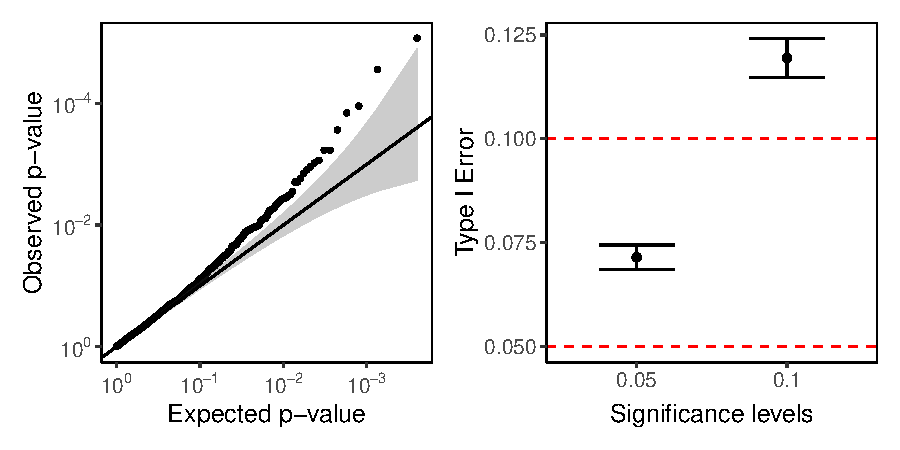
\includegraphics[width=0.95\textwidth]{figures-and-tables/auxiliary/failure_Hadad.pdf}
	\caption{Type-I error inflation using normal approximation in \citet{Hadad2021}. The simulation is repeated for $2000$ times.}
	\label{fig:failure_Hadad}
\end{figure}



\subsection{Investigating \citet{Hirano2023,adusumilli2023optimal}}

To address non-normality directly, \citet{Hirano2023} develop asymptotic representations for a broad class of test statistics under batched designs, which are subsequently used to derive power functions and optimal tests in \citet{adusumilli2023optimal}. The validity of this theory requires establishing weak convergence of a vector of statistics, as well as assuming that the potential outcome distributions are differentiable in quadratic mean (QMD). In contrast, our Theorem~\ref{thm:weak_convergence_W_N} focuses on the widely used WIPW class of statistics and provides explicit weak convergence results that go beyond the QMD framework, based on transparent and interpretable assumptions. 

\subsection{Investigating \citet{che2023adaptive}}\label{sec:inspection_Che}

While \citet{che2023adaptive} broaden the framework of \citet{Hirano2023} to encompass settings beyond QMD, 
their emphasis lies in experimental design within batched bandit designs rather than in inferential validation. Specifically, they analyze the statistic  
\[
\frac{1}{\sqrt{N_t}}\sum_{u=1}^{N_t}A_{uN}^{(t)}\,Y_{uN}^{(t)},
\]  
deriving its asymptotic distribution under conditions similar to ours. Their results, 
however, are not sufficient for the purpose of inference.
For example, one can show that—after an additional scaling by $\sqrt{N_t}$—this statistic generally fails to converge to the target estimand $\E[Y_{uN}(s)]$, except in the degenerate case $\E[Y_{uN}(s)]=0$.
Moreover, the asymptotic distribution therein contains unknown parameters, 
making it infeasible to construct valid hypothesis tests or confidence intervals based on this statistic.

By contrast, our work prioritizes the inferential integrity of adaptive experiments. Our results incorporate consistent and pivotal estimators, which
guarantees that hypothesis tests are valid and that confidence intervals faithfully reflect uncertainty around the desired parameter.



\section{Probabilistic preliminaries}\label{sec:auxiliary_Notation}

In Section~\ref{sec:BL_distance}, we discuss technique of proving weak convergence of random variables with test functions. In Section~\ref{sec:RCD_preliminary}, we discuss the regular conditional distribution (RCD) and its properties. 

\subsection{Bounded Lipschitz test function class}\label{sec:BL_distance}


We will use the following definition of convergence in distribution throughout the appendix.
\begin{definition}[Convergence in distribution]\label{def:convergence_distribution}
	Suppose $W_N\in\mathbb{R}^d$ is a sequence of random variables and $W\in\mathbb{R}^d$ is a random variable. We say $W_N$ converge in distribution to $W$ if for any bounded and continuous function $f:\mathbb{R}^d\rightarrow \mathbb{R}$, we have
	\begin{align*}
		\E[f(W_N)]\rightarrow \E[f(W)].
	\end{align*}
	Moreover, we use the notation $W_N\convd W$ to denote the convergence in distribution. If $W_N$ and $W$ are univariate, we will interchangeably use the following equivalent deifnition
	\begin{align*}
		\P[W_N\leq t]\rightarrow \P[W\leq t], \ \text{for each } t \in \R \text{ at which } t \mapsto \P[W \leq t] \text{ is continuous.}
	\end{align*}
\end{definition}

Beyond the bounded continuous functions, there are other classes of functions that are useful in the context of weak convergence. In particular, we will use the bounded Lipschitz function class to prove our main results. Suppose $f$ is a function from $\mathbb{R}^d$ to $\mathbb{R}$. We call $f$ is a $m$-Lipschitz function as long as $\|f\|_{\mathrm{L}}\leq m$, where \(\|f\|_{\mathrm{L}} \equiv \sup_{x \neq y \in \mathbb{R}^d} |f(x) - f(y)| / \|x - y\|_2\) and $\|\cdot\|_2$ is the Euclidean norm. Then we define 
\begin{align*}
	\|f\|_{\mathrm{BL}}\equiv \|f\|_{\mathrm{L}}+\|f\|_{\infty}\quad\text{where}\quad \|f\|_{\infty}\equiv \sup_{x\in\mathbb{R}^d}|f(x)|.
\end{align*}
\noindent The following lemma shows that the BL function class is rich enough to characterize the weak convergence of random variables.
\begin{lemma}[Theorem 11.3.3 in \citet{Dudley_2002}]\label{lem:Dudley_equivalence}
	Suppose the sequence of random variable $W_N\in\mathbb{R}$ and $W\in\mathbb{R}$ have law $\P_N$ and $\P$, respectively. Then the following two statements are equivalent:
	\begin{enumerate}
		\item $W_N\convd W$;
		\item $\left|\int f(x)\mathrm{d}\P_N(x)-\int f(x)\mathrm{d}\P(x)\right|\rightarrow0$ for any $f$ such that $\|f\|_{\mathrm{BL}}<\infty$.
	\end{enumerate}
\end{lemma}

Despite the fruitful results in the literature on normal approximation on independent observations \citep{chatterjee2008multivariate} and weakly dependent observation \citet{chen2004normal}, these existing results do not apply directly to our case since the adaptive sampling scheme introduces a \textit{strong} dependence structure. We will develop new tools for proving our results, based on these existing results. Thus we review the relevant results in the following section. First comes the finite-sample bound proved in \citet{chatterjee2008multivariate} and an interpolation result \citet{Meckes2009}.



\begin{lemma}[\citet{chatterjee2008multivariate}, Theorem 3.1]\label{lem:CLT_BL_distance}
	Let $W_{1N},\ldots, W_{NN}$ be a sequence of independent, identically distributed random vectors in $\mathbb{R}^k$. Suppose
	\begin{align*}
		\E[W_{uN}]=0,\ \E[W_{uN}W_{uN}^\top ]=\bm I_{k}.
	\end{align*}
	Let $W_N\equiv \sum_{u=1}^N W_{uN}/\sqrt{N}$ and $Z\sim N(\bm 0,\bm I_k)$. Then for any $g\in\mathcal{C}^2(\mathbb{R}^k)$,
	\begin{align*}
		\left|\E[g(W_N)]-\E[g(Z)]\right|\leq \frac{\|g\|_{\mathrm{L}}}{2\sqrt{N}}(\E[\|W_{uN}\|_2^4])^{1/2}+\frac{\sqrt{2\pi}}{3\sqrt{N}}\|\nabla g\|_{\mathrm{L}}\E[\|W_{uN}\|_2^3].
	\end{align*}
\end{lemma}

\noindent Lemma~\ref{lem:CLT_BL_distance} shows that when the test function is chosen to be $\mathcal{C}^2$, the weak convergence for $W_N$ can be derived as long as the third moment of $W_{uN}$ diverging slower than $\sqrt{N}$ and fourth moment diverging slower than $N$. 

\begin{lemma}[\citet{Meckes2009}, Corollary 3.5]\label{lem:smoothing}
	Consider the density function of a multivariate Gaussian random variable $\phi_{\delta}(x)\equiv \frac{1}{(2\pi \delta^2)^{k/2}}\exp\left(-\frac{1}{2\delta^2}\|x\|_2^2\right)$. For any $1$-Lipschitz function $f$, consider the Gaussian convolution $(f*\phi_{\delta})\equiv \E[f(x+\delta Z)]$ where $Z\sim N(\bm0,\bm I_k)$ and $\delta>0$. Then we have 
	\begin{align*}
		\|\nabla (f*\phi_{\delta})\|_{\mathrm{L}}\leq \|f\|_{\mathrm{L}}\times \sup_{\theta:\|\theta\|_2=1}\left\|\nabla \phi_{\delta}^\top\theta\right\|_1\leq \frac{\sqrt{2}}{\pi^{1/2}}\frac{1}{\delta}
	\end{align*}
	where $\|f\|_1$ denotes the $L_1$ norm of function $f$. Moreover, for any random variable $X$
	\begin{align*}
		\E[(f*\phi_{\delta})(X)-f(X)]\leq \E[\delta\|Z\|_2]\leq \delta\sqrt{k}.
	\end{align*}
\end{lemma}

\noindent Applying a smoothing argument to the Lipschitz function class with the help of Lemma \ref{lem:smoothing}, we can prove the weak convergence of $W_N$ under Lipschitz class with the same requirement on the third and fourth moment as in Lemma~\ref{lem:CLT_BL_distance}. We formalize such result in the following lemma.


\begin{lemma}[Upper bound with bounded Lipschitz function]\label{lem:W_1_bound}
	Suppose $W_{uN}\in\mathbb{R}^k$ are i.i.d. random variables for any fixed $N\in\mathbb{N}_+$. Then if we have $\E[W_{uN}]=\bm 0,\E[W_{uN}W_{uN}^\top]=\bm I_k$ and 
	\begin{align*}
		\frac{\E\left[\|W_{uN}\|_2^4\right]}{N}\rightarrow 0,\ \frac{\E[\|W_{uN}\|_2^3]}{N^{1/2}}\rightarrow0,
	\end{align*}
	then for any sequence of Lipschitz function $r_N$ such that $\|r_N\|_{\mathrm{BL}}\leq 1$, we have
	\begin{align*}
		\left|\E\left[r_N\left(\frac{1}{\sqrt{N}}\sum_{u=1}^N W_{uN}\right)\right]-\E\left[r_N\left(Z\right)\right]\right|\rightarrow0,\ Z\sim N(\bm 0,\bm I_k).
	\end{align*}
\end{lemma}



\subsection{Preliminaries on regular conditional distribution}\label{sec:RCD_preliminary}

To better understand the argument involving conditional distribution, we briefly discuss the basic definition of regular conditional distribution. Let $\mathcal{B}(\mathbb{R}^N)$ be the Borel $\sigma$-algebra on $\mathbb{R}^N$ and $\Omega,\mathcal{F}_N$ be the sample space and a sequence of $\sigma$-algebras. For any $N\in\mathbb{N}_+,\kappa_N:\Omega\times \mathcal{B}(\mathbb{R}^N)$ is a regular conditional distribution of $W_N\equiv (W_{1N},\ldots,W_{NN})$ given $\mathcal{F}_N$ if 
\begin{align*}
	\omega\mapsto \kappa_N(\cdot,B) \text{ is measurable with respect to $\mathcal{F}_N$ for any fixed $B\in\mathcal{B}(\mathbb{R}^N)$};
	&
	\\
	B\mapsto \kappa_N(\omega,B) \text{ is a probability measure on }(\mathbb{R}^N,\mathcal{B}(\mathbb{R}^N)) \text{ for any }\omega\in\Omega;
	&
	\\
	\kappa_N(\omega,B)=\P[(W_{1N},\ldots,W_{NN})\in B|\mathcal{F}_N](\omega)\text{ for almost all }\omega\in\Omega\text{ and all }B\in\mathcal{B}(\mathbb{R}^N).&
\end{align*}
The following lemma from \citet[Theorem 8.37]{Lista2017} ensures the general existence of regular conditional distribution.
\begin{lemma}[Theorem 8.37 in \citet{Lista2017}]\label{lem:Klenke_Thm_8.37}
  Suppose $(\Omega,\mathcal{G},\P)$ is the Probability triple. Let $\mathcal{F}\subset \mathcal{G}$ be a sub-$\sigma$-algebra. Let $Y$ be a random variable with values in a Borel space $(E,\mathcal{E})$ (for example, $E$ is Polish, $E=\mathbb{R}^k$). Then there exists a regular conditional distribution $\kappa_{Y,\mathcal{F}}$ of $Y$ given $\mathcal{F}$.
\end{lemma}
\noindent Result from \citet[Theorem 8.38]{Lista2017} guarantees that the conditional expectation and the integral of measurable function with respect to regular conditional distribution are almost surely same.

\begin{lemma}[Modified version of Theorem 8.38 in \citet{Lista2017}]\label{lem:Klenke_Thm_8.38}
  Let $Y$ be a random variable $(\Omega,\mathcal{G},\mathbb{P})$ taking values in a Borel space $(E,\mathcal{E})$. Let $\mathcal{F}\subset \mathcal{G}$ be a $\sigma$-algebra and let $\kappa_{Y,\mathcal{F}}$ be a regular conditional distribution of $Y$ given $\mathcal{F}$. Further, let $f:E\rightarrow\mathbb{R}$ be measurable and $\E[|f(Y)|]<\infty$. Then we can define a version of the conditional expectation using regular conditional distribution, i.e., 
  \begin{align*}
    \E[f(Y)|\mathcal{F}](\omega)=\int f(y)\mathrm{d}\kappa_{Y,\mathcal{F}}(\omega,y),\ \forall \omega\in\Omega.
  \end{align*}
\end{lemma}
\noindent Throughout this paper we will fix a version of the conditional expectation and the version is defined by applying Lemma \ref{lem:Klenke_Thm_8.38}. The following lemma is useful as well. 

\begin{lemma}[Conditional expectation with variable measurable with respect to $\mathcal{F}$]\label{lem:new_klenke_thm_8.38}
	Let $Y$ be a random variable $(\Omega,\mathcal{G},\mathbb{P})$ with values in a Borel space $(E,\mathcal{E})$. Let $\mathcal{F}\subset \mathcal{G}$ be a $\sigma$-algebra and let $\kappa_{Y,\mathcal{F}}$ be a regular conditional distribution of $Y$ given $\mathcal{F}$. Suppose $X\in\mathcal{F}$ is a random variable in another Borel space $(B,\mathcal{B})$. Further, let $f:E\times B\rightarrow\mathbb{R}$ be measurable and $\E[|f(X, Y)|]<\infty$. Then we can define a version of the following conditional expectation using regular conditional distribution:
  \begin{align*}
    \E[f(X, Y)|\mathcal{F}](\omega)=\int f(X(\omega),y)\mathrm{d}\kappa_{Y,\mathcal{F}}(\omega,y),\ \forall \omega\in\Omega.
  \end{align*}
\end{lemma}

\subsection{Definition of conditional convergence}



Since we are under the setup where the data is generated adaptively, we need to extensively work with the conditional convergence where the conditioning is on the data collected in the first stage. We need to first define the notions of conditional convergence, with the definition of regular conditional distribution. In particular, we adopt the definition of conditional convergence in distribution and probability from \citet{niu2024reconciling}.


\begin{definition} \label{def:conditional-convergence-distribution}
    For each $N$, let $W_N$ be a random variable and let $\mathcal F_N$ be a $\sigma$-algebra. Then, we say $W_N$ converges in distribution to a random variable $W$ conditionally on $\mathcal F_N$ if
    \begin{equation}
        \P[W_N \leq t \mid \mathcal F_N] \convp \P[W \leq t] \ \text{for each } t \in \R \text{ at which } t \mapsto \P[W \leq t] \text{ is continuous.}
    \end{equation}
    We denote this relation via $W_N \mid \mathcal F_N \convdp W$.
\end{definition}

\begin{definition} \label{def:conditional-convergence-probability}
	For each $N$, let $W_N$ be a random variable and let $\mathcal F_N$ be a $\sigma$-algebra. Then, we say $W_N$ converges in probability to a constant $c$ conditionally on $\mathcal F_N$ if $W_N$ converges in distribution to the delta mass at $c$ conditionally on $\mathcal F_N$ (recall Definition~\ref{def:conditional-convergence-distribution}). We denote this convergence by ${W_N \mid \mathcal F_N \convpp c}$. In symbols, 
	\begin{equation}
		W_N \mid \mathcal F_N \convpp c \quad \text{if} \quad W_N \mid \mathcal F_N \convdp \delta_c.
	\end{equation}
\end{definition}



\subsection{Proof of Lemma \ref{lem:W_1_bound}}

\begin{proof}[Proof of Lemma \ref{lem:W_1_bound}]
	Define the Gaussian convolution of $r_N(x)$ as $F_N(x,\delta)\equiv \E[r_N(x+\delta Y)]$ where $Y\sim N(\bm 0,\bm I_k)$ and the expectation is taken with respect to $Y$. We first decompose the desired difference to three parts: 
	\begin{align*}
		A_N
		&
		\equiv \E\left[r_N\left(\frac{1}{\sqrt{N}}\sum_{u=1}^N W_{uN}\right)\right]-\E\left[r_N\left(Z\right)\right]\\
		&
		=\E\left[r_N\left(\frac{1}{\sqrt{N}}\sum_{u=1}^N W_{uN}\right)\right]-\E\left[F_N\left(\frac{1}{\sqrt{N}}\sum_{u=1}^N W_{uN},\delta\right)\right]\\
		&
		\quad +\E\left[F_N\left(\frac{1}{\sqrt{N}}\sum_{u=1}^N W_{uN},\delta\right)\right]-\E\left[F_N\left(Z,\delta\right)\right]\\
		&
		\quad +\E\left[F_N\left(Z,\delta\right)\right]-\E\left[r_N\left(Z\right)\right]\\
		&
		\equiv A_N^{(1)}+A_N^{(2)}+A_N^{(3)}.
	\end{align*}
	\noindent Now we decompose the proof into two steps. 
	
	\paragraph{Control of $A_{N}^{(2)}$:}
	
	We want to apply Lemma \ref{lem:CLT_BL_distance} and \ref{lem:smoothing} to the variables $W_{uN}$. First we notice for any fixed $N$ and $\delta,F_N(x,\delta)\in \mathcal{C}^2(\mathbb{R}^k)$. Indeed, we can write, by change of variable,
	\begin{align*}
		F_N(x,\delta)=\E[r_N(x+\delta A)]=\int r_N(x+\delta a)\phi(a)da=\int r_N(t)\frac{1}{\delta^d}\phi\left(\frac{t-x}{\delta}\right)\mathrm{d}t.
	\end{align*}
	By dominated convergence theorem, we can interchange the derivative and integral so that we can verify for any fixed $N,\delta,F_N(x,\delta)$ is 2-times continuously differentiable. Then applying Lemma \ref{lem:CLT_BL_distance} with $W_{uN}$, we have
	\begin{align*}
		|A_{N}^{(2)}|\leq \frac{\|F_N(\cdot, \delta)\|_{\mathrm{L}}\left(\E[\|W_{uN}\|_2^4]\right)^{1/2}}{2N^{1/2}}+\frac{\sqrt{2\pi}\|\nabla F_N(\cdot, \delta)\|_{\mathrm{L}}\E[\|W_{uN}\|_2^3]}{3N^{1/2}}.
	\end{align*}
	By the definition of $r_N$ that $\|r_N\|_{\mathrm{BL}}\leq 1$ so that $\|F_N(\cdot, \delta)\|_{\mathrm{L}}\leq 1$. Then applying Lemma \ref{lem:smoothing}, we obtain $\|\nabla F_N(\cdot, \delta)\|_{\mathrm{L}}\leq \sqrt{2}/(\pi^{1/2}\delta)$.
	Therefore we have 
	\begin{align*}
		|A_{N}^{(2)}|\leq \frac{1}{2}\frac{\left(\E[\|W_{uN}\|_2^4]\right)^{1/2}}{N^{1/2}}+\frac{2}{3\delta}\frac{\E[\|W_{uN}\|_2^3]}{N^{1/2}}.
	\end{align*}
	
	\paragraph{Control of $A_{N}^{(1)},A_{N}^{(3)}$:}
	Applying Lemma \ref{lem:smoothing}, we know $|A_{N}^{(1)}|\leq \delta \sqrt{k},\ |A_{N}^{(3)}|\leq \delta \sqrt{k}$.
	
	\paragraph{Conclusion:}
	
	Collecting all the results above, we have 
	\begin{align*}
		|A_{N}|\leq \frac{1}{2}\frac{\left(\E[\|W_{uN}\|_2^4]\right)^{1/2}}{N^{1/2}}+\frac{2}{3\delta}\frac{\E[\|W_{uN}\|_2^3]}{N^{1/2}}+2\delta \sqrt{k}.
	\end{align*}
	Since 
	\begin{align*}
		\frac{\E[\|W_{uN}\|_2^4]}{N}\rightarrow 0,\ \frac{\E[\|W_{uN}\|_2^3]}{N^{1/2}}\rightarrow 0, \text{ almost surely}
	\end{align*}
	as assumed, we can optimize $\delta$ such that $|A_N|\rightarrow 0$ to complete the proof.
\end{proof}



\subsection{Proof of Lemma \ref{lem:new_klenke_thm_8.38}}

\begin{proof}[Proof of Lemma \ref{lem:new_klenke_thm_8.38}]
	By Lemma \ref{lem:Klenke_Thm_8.38}, we know that 
	\begin{align*}
		\E[f(X,Y)|\mathcal{F}](\omega)=\int f(x,y)\mathrm{d}\kappa_{(X,Y),\mathcal{F}}(\omega,(x,y)).
	\end{align*}
	Now we prove that for almost every $\omega\in\Omega$,
	\begin{align*}
		\kappa_{(X,Y),\mathcal{F}}(\omega,S)=\kappa_{Y,\mathcal{F}}(\omega,S_1)\cdot \indicator(X(\omega)\in S_2),\ \forall S=S_1\times S_2\subset E\times B.
	\end{align*}
	In other words, $\kappa_{(X,Y),\mathcal{F}}(\omega,\cdot)$ is product measure of another measure $\kappa_{Y,\mathcal{F}}(\omega,\cdot)$ and counting measure supported on the value $X(\omega)$. This can be proved by using the definition of regular conditional distribution. For any $S=S_1\times S_2\subset E\times B$, we have
	\begin{align*}
		\kappa_{(X,Y),\mathcal{F}}(\omega,S)=\P[(X,Y)\in S|\mathcal{F}](\omega)
		&
		=\indicator(X(\omega)\in S_2)\P[Y\in S_1|\mathcal{F}](\omega)\\
		&
		=\kappa_{Y,\mathcal{F}}(\omega,S_1)\cdot \indicator(X(\omega)\in S_2)
	\end{align*}
	for almost every $\omega\in\Omega$. Thus by Fubini's theorem, we conclude
	\begin{align*}
		\int f(x,y)\mathrm{d}\kappa_{(X,Y),\mathcal{F}}(\omega,(x,y))=\int f(X(\omega),y)\mathrm{d}\kappa_{Y,\mathcal{F}}(\omega,y).
	\end{align*}
\end{proof}


\section{Useful lemmas and the proofs}\label{sec:aux_lemma}


\subsection{Lemma statements}

\begin{lemma}[Conditional Polya's theorem, Theorem 5 in \citet{niu2024reconciling}]\label{lem:cond_polya} 
	Let $W_N$ be a sequence of random variables. If $W_N \mid \mathcal F_N \convdp W$ for some random variable $W$ with continuous CDF, then
	\begin{equation}
		\sup_{t \in \R}|\P[W_N \leq t \mid \mathcal F_N] - \P[W \leq t]| \convp 0.
	\end{equation}
\end{lemma}


\begin{lemma}[Slutsky's theorem, Theorem 13.18 in \citet{Dudley_2002}]\label{lem:Slutsky}
	Let $X_1,X_2\ldots$ and $Y_1,Y_2,\ldots,$ be random variables with values in $\mathbb{R}^{k}$. Suppose $X_N\convd X$ and $\|X_N-Y_N\|_2\convp 0$. Then $Y_N\convd X$.
\end{lemma}






\begin{lemma}[Conditional weak law of large numbers, Theorem 7 in \citet{niu2024reconciling}] \label{lem:wlln_conditional} 
	Let $W_{uN}$ be a triangular array of random variables, such that $W_{uN}$ are independent conditionally on $\mathcal F_N$ for each $N$. If for some $\delta > 0$ we have
	\begin{equation}
		\frac{1}{N^{1+\delta}}\sum_{u=1}^N\E[|W_{uN}|^{1+\delta}\mid\mathcal{F}_N] \convp 0,
		\label{eq:wlln_cond_assumption}
	\end{equation}
	then 
	\begin{equation}
		\frac{1}{N} \sum_{u = 1}^N (W_{uN} - \E[W_{uN}|\mathcal{F}_N]) \mid \mathcal F_N \convpp 0.
		\label{eq:wlln_cond_conclusion}
	\end{equation}
	Applying the dominated convergence theorem, we know 
	\begin{align*}
		\frac{1}{N} \sum_{u = 1}^N (W_{uN} - \E[W_{uN}|\mathcal{F}_N])\convp 0.
	\end{align*}
	The condition~\eqref{eq:wlln_cond_assumption} is satisfied when
	\begin{equation}
		\sup_{1\leq u\leq N}\E[|W_{uN}|^{1+\delta} \mid \mathcal{F}_N]=o_p(N^{\delta}).
		\label{eq:wlln_cond_sufficient}
	\end{equation}
\end{lemma}


\begin{lemma}[\citet{durrett2019probability}, Theorem 2.3.2]\label{lem:sub_subseq}
	A sequence of random variables $W_N$ converges to a limit $W$ in probability if and only if every subsequence of $W_N$ has a further subsequence that converges to $W$ almost surely.
\end{lemma}

\begin{lemma}[Skorohod's representation theorem]\label{lem:skorohod}
	Let \( (\mu_N)_{N \in \mathbb{N}} \) be a sequence of probability measures on a metric space \( S \) such that \( \mu_N \) converges weakly to some probability measure \( \mu_{\infty} \) on \( S \) as \( N\to \infty \). Suppose also that the support of \( \mu_{\infty} \) is separable. Then there exist \( S \)-valued random variables \( W_N \) defined on a common probability space \( (\Omega, \mathcal{F}, \P) \) such that the law of \( W_N \) is \( \mu_N \) for all \( N \) (including \( N = \infty \)) and such that \( (W_N)_{N \in \mathbb{N}} \) converges to \( W_{\infty} \), \( \P \)-almost surely.
\end{lemma}

%   \begin{lemma}[\citet{bhattacharya1970rates}, Theorem 1; \citet{che2023adaptive}, Lemma 7]\label{lem:bhattacharya_lemma}
% 	Let $\{X_{uN}\}_{u=1}^N$ be a sequence of $N$ independent random vectors taking values in $\mathbb{R}^{k}$ with covariance matrix $\bm\Sigma_N$. Assume that for some $\delta>0$ we have 
% 	\begin{align*}
% 		M\equiv \sup_{N}\frac{1}{N}\sum_{u=1}^N\E\left(\left\|\bm\Sigma_N^{-1/2}X_{uN}\right\|_2^{3+\delta}\right)<\infty.
% 	\end{align*}
% 	Then the normalized partial sum $\bar Z_N\equiv\sum_{u=1}^N \bm\Sigma_{N}^{-1/2}X_{uN}$ satisfies 
% 	\begin{align*}
% 		\mathrm{d}_{\mathrm{BL}}(\bar Z_N, N(0,\bm I_k))\leq A_{K,\delta}M^{(3+3\delta)/(3+\delta)}N^{-1/2}+B_{K,\delta}M^{3/(3+\delta)}N^{-1/2}
% 	\end{align*}
% 	where 
% 	\begin{align*}
% 		\mathrm{d}_{\mathrm{BL}}(\mu,\nu)\equiv\sup\left\{\E_{\mu}[f(X)]-\E_{\nu}[f(X)]:f\in\mathrm{Lip}(\mathbb{R}^{k}),\sup_{x,y\in\mathbb{R}^{k}}|f(x)-f(y)|\leq 1\right\}.
% 	\end{align*}
% \end{lemma}


\begin{lemma}[Lipschitz continuity of square root matrix under F-norm]\label{lem:holder_continuity_Frobenius}
	Suppose $A,B\in\mathbb{R}^{k\times k}$ are two positive definite matrices, then we have 
	\begin{align*}
		\|A^{1/2}-B^{1/2}\|_{\mathrm{F}}\leq \sqrt{k}\|A-B\|_{\mathrm{F}}^{1/2}.
	\end{align*}
\end{lemma}




\begin{lemma}[Boundedness on the covariance]\label{lem:upper_bound_cov}
	Suppose $X_N,Y_N$ are two sequences of random variables, with finite first moment, satisfying 
	\begin{enumerate}
		\item $\E[X_N^{p}]$ and $\E[Y_N^{p}]$ converge to finite constants for $p=1,2$;
		\item $\liminf_{N\rightarrow\infty}\mathrm{Var}[X_N]>0,\ \liminf_{N\rightarrow\infty}\mathrm{Var}[Y_N]>0$.
	\end{enumerate}
	Suppose a random sequence $a_N\in (0,1)$ almost surely. Then we have 
	\begin{align}\label{eq:upper_bound_cov}
		\limsup_{N\rightarrow\infty}\left|\frac{a_N^{1/2}\E[X_N]}{(\E[X_N^2]-a_N\E[X_N]^2)^{1/2}}\times \frac{(1-a_N)^{1/2}\E[Y_N]}{(\E[Y_N^2]-(1-a_N)\E[Y_N]^2)^{1/2}}\right|<C<1
	\end{align}
	almost surely and the constant $C$ only depends on the limit of the moments $\lim_{N\rightarrow\infty}\E[X_N^p]$ and $\lim_{N\rightarrow\infty}\E[Y_N^p]$ for $p\in\{1,2\}$.
\end{lemma}


\subsection{Proof of Lemma \ref{lem:holder_continuity_Frobenius}}

\begin{proof}[Proof of Lemma \ref{lem:holder_continuity_Frobenius}]
	It suffices to prove 
	\begin{align}\label{eq:holder_continuity_2_Norm}
		\|A^{1/2}-B^{1/2}\|_{2}\leq \|A-B\|_{2}^{1/2},
	\end{align}
	where $\|A\|_2$ is the operator norm $A$. This is because if the statement~\eqref{eq:holder_continuity_2_Norm} holds, then
	\begin{align*}
		\|A^{1/2}-B^{1/2}\|_{\mathrm{F}}\leq \sqrt{k}\|A^{1/2}-B^{1/2}\|_{2}\leq \sqrt{k}\|A-B\|_{2}^{1/2}\leq \sqrt{k}\|A-B\|_{\mathrm{F}}^{1/2}.
	\end{align*}
	Now we prove \eqref{eq:holder_continuity_2_Norm}. If vector $x$ with $\|x\|=1$ is an eigenvector of $\sqrt{A}-\sqrt{B}$ with eigenvalue $\mu$ then 
	\begin{align*}
		x^\top (A-B)x=x^\top (\sqrt{A}-\sqrt{B})\sqrt{A}x+x^\top \sqrt{B}(\sqrt{A}-\sqrt{B})x=\mu x^\top (\sqrt{A}+\sqrt{B})x.
	\end{align*}
	Now if we choose $\mu=\pm \|\sqrt{A}-\sqrt{B}\|_2$ (depending on the sign of the eigenvalue which has the largest magnitude), we have
	\begin{align*}
		\|\sqrt{A}-\sqrt{B}\|_2^2=(x^\top (\sqrt{A}-\sqrt{B})x)^2
		&
		\leq |x^\top (\sqrt{A}-\sqrt{B})x|x^\top (\sqrt{A}+\sqrt{B})x\\
		&
		=|x^\top (A-B)x|\leq \|A-B\|_2.
	\end{align*}
	This completes the proof.
\end{proof}


\subsection{Proof of Lemma \ref{lem:upper_bound_cov}}

\begin{proof}[Proof of Lemma \ref{lem:upper_bound_cov}]

	We now divide the proof into two cases.
	\begin{enumerate}
		\item \textbf{When $\lim_{N\rightarrow\infty}\E[X_N]=0$ or $\lim_{N\rightarrow\infty}\E[Y_N]=0$.} Since 
	\begin{align*}
		\liminf_{N\rightarrow\infty}(\E[X_N^2]-a_N\E[X_N]^2)\geq \liminf_{N\rightarrow\infty}(\E[X_N^2]-\E[X_N]^2)>0
	\end{align*}
	and 
	\begin{align*}
		\liminf_{N\rightarrow\infty}(\E[Y_N^2]-(1-a_N)\E[Y_N]^2)\geq \liminf_{N\rightarrow\infty}(\E[Y_N^2]-\E[Y_N]^2)>0,
	\end{align*}
	we know the claim is true with $C=0$ almost surely.
	\item\textbf{When both $\lim_{N\rightarrow\infty}\E[X_N]\neq 0$ and $\lim_{N\rightarrow\infty}\E[Y_N]\neq 0$:} Define the sequence $E_N\equiv a_N\E[Y_N^2](\E[X_N^2]-\E[X_N^2]) +(1-a_N)(\E[Y_N^2]-\E[Y_N]^2)\E[X_N^2]$. We know 
	\begin{align*}
		D_N 
		&
		\equiv (\E[X_N^2]-a_N\E[X_N]^2)(\E[Y_N^2]-(1-a_N)\E[Y_N]^2)\\
		&
		= a_N(1-a_N)(\E[X_N]\E[Y_N])^2+ E_N\\
		&
		\equiv C_N +E_N,
	\end{align*}
	Note that conclusion~\eqref{eq:upper_bound_cov} is equivalent to proving $\limsup_{N\rightarrow\infty}|C_N^{1/2}/D_N^{1/2}|<1$ almost surely. To this end, we observe that
	\begin{align*}
		\frac{D_N}{C_N}
		&
		=1+\frac{E_N}{C_N}\\
		&
		=1+\frac{a_N\E[Y_N^2](\E[X_N^2]-\E[X_N]^2)}{C_N}+\frac{(1-a_N)(\E[Y_N^2]-\E[Y_N]^2)\E[X_N^2]}{C_N}\\
		&
		=1+\frac{\E[Y_N^2](\E[X_N^2]-\E[X_N]^2)}{(1-a_N)(\E[X_N]\E[Y_N])^2}+\frac{(\E[Y_N^2]-\E[Y_N]^2)\E[X_N^2]}{a_N (\E[X_N]\E[Y_N])^2}\\
		&
		\equiv 1+R_{1N}+R_{2N}.
	\end{align*}
	We can bound 
	\begin{align*}
		\liminf_{N\rightarrow\infty}R_{1N}
		&
		\geq \liminf_{N\rightarrow\infty}\frac{\E[Y_N^2](\E[X_N^2]-\E[X_N]^2)}{(\E[X_N]\E[Y_N])^2}\\
		&
		=\lim_{N\rightarrow\infty}\frac{\E[Y_N^2]}{(\E[Y_N])^2}\lim_{N\rightarrow\infty}\frac{(\E[X_N^2]-\E[X_N]^2)}{(\E[X_N])^2}>0
	\end{align*}
	almost surely, since $\lim_{N\rightarrow\infty}(\E[X_N^2]-\E[X_N]^2)=\lim_{N\rightarrow\infty}\mathrm{Var}[X_N]>0$. Similarly, we can prove $\liminf_{N\rightarrow\infty}R_{2N} >0$ almost surely. Thus we have 
	\begin{align*}
		\liminf_{N\rightarrow\infty}\frac{D_N}{C_N}\geq 1+\liminf_{N\rightarrow\infty}R_{1N}+\liminf_{N\rightarrow\infty}R_{2N}>1
	\end{align*}
	almost surely. Thus the desired bound can be obtained by checking
	\begin{align*}
		&
		\limsup_{N\rightarrow\infty}\left|\frac{a_N^{1/2}\E[X_N]}{(\E[X_N^2]-a_N\E[X_N]^2)^{1/2}}\times \frac{(1-a_N)^{1/2}\E[Y_N]}{(\E[Y_N^2]-(1-a_N)\E[Y_N]^2)^{1/2}}\right|\\
		&
		=
		\limsup_{N\rightarrow\infty}\left|\frac{C_N^{1/2}}{D_N^{1/2}}\right|=\frac{1}{\liminf_{N\rightarrow\infty}D_N^{1/2}/C_N^{1/2}}<1
	\end{align*}
	almost surely.
	\end{enumerate}
	
\end{proof}



\section{New results on conditional CLT and CMT}\label{sec:new_conditional_CLT}


In this section, we present a new conditional central limit theorem (CLT) and a new continuous mapping theorem (CMT) under the conditional convergence framework. 

\subsection{A new conditional CLT}


\begin{lemma}[Conditional CLT under Lipschitz class]\label{lem:CLT_BL}
	Consider $\sigma$-alegbras $\mathcal{F}_N$. Suppose $W_{1N},\ldots,W_{NN}\in\mathbb{R}^k$ are i.i.d. random variables conditional on $\mathcal{F}_N$ for any fixed $N\in\mathbb{N}$. Define $W_N\equiv \sum_{u=1}^N W_{uN}/\sqrt{N}$.  Suppose
	\begin{align*}
		\E[W_{uN}|\mathcal{F}_N]=\bm 0,\ \E[W_{uN}W_{uN}^\top|\mathcal{F}_N]=\bm I_{k}
	\end{align*}
	and 
	\begin{align*}
		\frac{\E[\|W_{uN}\|_2^4|\mathcal{F}_N]}{N}=o_p(1),\ \frac{\E[\|W_{uN}\|_2^3|\mathcal{F}_N]}{\sqrt{N}}=o_p(1).
	\end{align*}
	Furthermore, consider random variables $X_N\in\mathbb{R}^k$ and $X_N$ is measurable with respect to $\mathcal{F}_N$. Then for any measurable function $g_N:\mathbb{R}^k\mapsto\mathbb{R}^d$ and any Lipschitz function $f:\mathbb{R}^{d+k}\rightarrow\mathbb{R}$ such that $\|f\|_{\mathrm{BL}}\leq 1$, we have
	\begin{align*}
		\E[f(g_N(X_N),W_N)|\mathcal{F}_N]-\E[f(g_N(X_N),Z)|\mathcal{F}_N]=o_p(1)\quad\text{where}\quad Z\sim N(0,\bm I_{k}).
	\end{align*}
\end{lemma}

\noindent Lemma \ref{lem:CLT_BL} can be viewed a conditional version of Lemma \ref{lem:W_1_bound}.

\subsection{New conditional CMT results}\label{sec:conditional_CMT}

In this section, we extend the classical continuous mapping theorem to conditional convergence. The following lemma is the classical result.

\begin{lemma}[Classical CMT]\label{lem:continuous_mapping_lem}
	Let $W_N,W$ be random variables on a metric space $S$. Suppose a function $g:S\mapsto S'$, where $S'$ is another metric space, has the set of discontinuity points $D_g$ such that $\P[W\in D_g]=0$. Then if $W_N\convd W$, the following is true: $g(W_N)\convd g(W)$.
\end{lemma}

\noindent To account for the varying sequence and conditioning, we present the following lemmas. These wo results provide new conditional convergence in probability and distribution, respectively. 

\begin{lemma}[CMT: convergence in conditional probability]\label{lem:continuous_map_varying}
	Suppose $X_N,Y_N\in\mathcal{X}\subset \mathbb{R}^k$ and $\|X_N-Y_N\|_2=o_p(1)$. Furthermore, suppose function $f:\mathcal{X}\rightarrow\mathbb{R}$ is uniformly continuous in the support $\mathcal{X}$ and uniformly bounded: $\sup_{x\in\mathcal{X}}|f(x)|<\infty$. Then we have $\E[\left|f(X_N)-f(Y_N)\right|]\rightarrow 0$. Moreover, we have $\E[\left|f(X_N)-f(Y_N)\right||\mathcal{F}_N]\convp 0$.
\end{lemma}

\begin{lemma}[CMT: convergence in conditional distribution]\label{lem:sufficient_condition_CMT}
	Consider the $\sigma$-algebra $\mathcal{F}_N$ and a measurable function $g$ with discontinuity set $D_g$. Suppose random variable $W\sim\mathbb{P}_W$ satisfies $\P[W\in D_g]=0$ and $g(W)$ is a continuous random variable. If the sequence of random variable $W_N$ satisfies
	\begin{align*}
		\left|\E[f(W_N)|\mathcal{F}_N]-\E[f(W)]\right|\convp 0, \text{ for any } f\text{ such that }\|f\|_{\mathrm{BL}}<\infty,
	\end{align*}
	then we have $\sup_{t\in\mathbb{R}}\left|\P[g(W_N)\leq t|\mathcal{F}_N]-\P[g(W)\leq t]\right|\convp 0$.
\end{lemma}


\subsection{Proof of Lemma \ref{lem:CLT_BL}}

\begin{proof}[Proof of Lemma \ref{lem:CLT_BL}]
	We prove the result by regular conditional distribution argument. Define the regular conditional distribution $\kappa_{\tilde W_N,\mathcal{F}_N}(\omega,\cdot)$ for $\tilde W_N=(W_{1N},\ldots,W_{NN})$ given $\mathcal{F}_N$ such that for almost every $\omega\in\Omega$, 
	\begin{align*}
		\kappa_{\tilde{W}_N,\mathcal{F}_N}(\omega,B)=\P[\tilde{W}_N\in B|\mathcal{F}_N](\omega),\forall B\in\mathcal{B}(\mathbb{R}^{Nk}).
	\end{align*}
	Now suppose $(\tilde{W}_{1N}(\omega),\ldots, \tilde{W}_{NN}(\omega))$ is a draw from $\kappa_{\tilde{W}_N,\mathcal{F}_N}(\omega,\cdot)$. Then by Lemma \ref{lem:new_klenke_thm_8.38} and \ref{lem:sub_subseq}, it suffices to prove for any subsequence $N_k$ of $N$, there exists a further subsequence $N_{k_j}$ such that for almost every $\omega\in\Omega$
	\begin{align*}
		A_{N_{k_j}}\equiv \int f\left(g_{N_{k_j}}(X_{N_{k_j}}(\omega)), x\right)\mathrm{d}\kappa_{\tilde{W}_N,\mathcal{F}_N}(\omega,x)-\int f\left(g_{N_{k_j}}(X_{N_{k_j}}(\omega)), Z\right)\mathrm{d}\mathbb{P}_Z\rightarrow 0,
	\end{align*}
	where $\mathbb{P}_Z$ is the law of $Z$. The way we choose the subsequence $N_{k_j}$ is to search $N_{k_j}$ such that
	\begin{align*}
		\frac{\E[\|W_{uN_{k_j}}\|_2^4|\mathcal{F}_{N_{k_j}}](\omega)}{N_{k_j}}\rightarrow 0,\ \frac{\E[\|W_{uN_{k_j}}\|_2^3|\mathcal{F}_{N_{k_j}}](\omega)}{N_{k_j}^{1/2}}\rightarrow 0,\text{ for almost every }\omega\in\Omega.
	\end{align*}
	This is doable guaranteed by the assumption in the lemma. We apply Lemma \ref{lem:W_1_bound} with $r_{N_{k_j}}(\cdot)=f(g_{N_{k_j}}(X_{N_{k_j}}(\omega)),\cdot)$ and $U_{uN_{k_j}}=\tilde{W}_{uN_{k_j}}(\omega)$ so that we have $A_{N_{k_j}}\rightarrow0$ almost surely. This completes the proof. 

\end{proof}

\subsection{Proof of Lemma \ref{lem:continuous_map_varying}}

\begin{proof}[Proof of Lemma \ref{lem:continuous_map_varying}]
	Fix any $\delta>0$, we can choose $\varepsilon(\delta)>0$ such that whenever $\|X_N-Y_N\|_2<\varepsilon(\delta)$ we can guarantee $|f(X_N)-f(Y_N)|\leq \delta$ since $f$ is uniformly continuous in $\mathcal{X}$. Then for any $\delta>0$, we have 
	\begin{align*}
		\E[\left|f(X_N)-f(Y_N)\right|]
		&
		= \E\left[|f(X_N)-f(Y_N)|\mathbf{1}(\|X_N-Y_N\|_2\leq \varepsilon(\delta))\right]\\
		&
		\qquad +\E\left[|f(X_N)-f(Y_N)|\mathbf{1}(\|X_N-Y_N\|_2>\varepsilon(\delta))\right]\\
		&
		\leq \delta+2\sup_{x\in\mathcal{X}}|f(x)|\P[\|X_N-Y_N\|_2>\varepsilon(\delta)].
	\end{align*}
	Letting $N\rightarrow\infty$, we know $\P[\|X_N-Y_N\|_2>\varepsilon(\delta)]\rightarrow0$ so that we have 
	\begin{align*}
		\lim_{N\rightarrow\infty}\E[\left|f(X_N)-f(Y_N)\right|]\leq \delta.
	\end{align*}
	Since $\delta$ is chosen arbitrarily, we have $\lim_{N\rightarrow\infty}\E[\left|f(X_N)-f(Y_N)\right|]=0$ so that we complete the first part proof. By the uniform integrability of $\E[|f(X_N)-f(Y_N)|\mathcal{F}_N]$, guaranteed by the uniform boundedness of $f$, we conclude the second part of the proof.
\end{proof}



\subsection{Proof of Lemma \ref{lem:sufficient_condition_CMT}}


\begin{proof}[Proof of Lemma \ref{lem:sufficient_condition_CMT}]
	Using Lemma \ref{lem:Klenke_Thm_8.38} and definition of regular conditional distribution, we know 
	\begin{align*}
		\left|\int f(x)\mathrm{d}\kappa_{W_N,\mathcal{F}_N}(\omega,x)-\int f(x)\mathrm{d}\mathbb{P}_W(x)\right|\rightarrow0,\text{ for any }f\text{ such that } \|f\|_{\mathrm{BL}}<\infty
	\end{align*}
	for any $\omega\in\mathcal{E}\subset\Omega$, where $\P[\mathcal{E}]\rightarrow1$. Applying Lemma \ref{lem:Dudley_equivalence} to $\kappa_{W_N,\mathcal{F}_N}(\omega,\cdot),\P_W(\cdot)$, we know on the event $\mathcal{E}$, random variable $\tilde{W}_N$ from measure $\kappa_{W_N,\mathcal{F}_N}(\omega,\cdot)$ converges to measure $\P_W(\cdot)$ in distribution. In other words, we have for any bounded and continuous function $h$,
	\begin{align*}
		\E[h(\tilde{W}_N(\omega))]=\int h(x)\mathrm{d}\kappa_{W_N,\mathcal{F}_N}(\omega,x)\rightarrow \int h(x)\mathrm{d}\mathbb{P}_W(x)=\E[h(W)],\ \forall \omega\in\mathcal{E}.
	\end{align*}
	Then by continuous mapping theorem, we have for any $t\in\mathbb{R}$,
	\begin{align*}
		\P[g(\tilde{W}_N(\omega))\leq t]\rightarrow \P[g( W)\leq t],\ \forall \omega\in\mathcal{E}\cap \{W\notin D_g\}.
	\end{align*}
	Again applying Lemma \ref{lem:Klenke_Thm_8.38}, we know $\forall \omega\in\mathcal{E}\cap \{W\notin D_g\}$,
	\begin{align*}
		\left|\P[g(W_N)\leq t|\mathcal{F}_N](\omega)-\P[g(W)\leq t]\right|\rightarrow 0.
	\end{align*}
	Since $\P[\mathcal{E}\cap \{W\notin D_g\}]=\P[\mathcal{E}]\rightarrow 1$ by the assumption that $\P[W\in D_g]=0$, we have 
	\begin{align*}
		\left|\P[g(W_N)\leq t|\mathcal{F}_N]-\P[g(W)\leq t]\right|\convp 0.
	\end{align*}
	Finally, applying Lemma \ref{lem:cond_polya}, we have
	\begin{align*}
		\sup_{t\in\mathbb{R}}\left|\P[g(W_N)\leq t|\mathcal{F}_N]-\P[g(W)\leq t]\right|\convp 0.
	\end{align*}
\end{proof}

\section{Preparation for the proof of Theorem~\ref{thm:weak_convergence_W_N}}


\subsection{Auxiliary definitions for the proof of Theorem~\ref{thm:weak_convergence_W_N}}\label{sec:notation_main_proof}

Recall the definition of $c_N$ and $c$ in Assumption~\ref{assu:moment_condition}. Then consider the function $h(\cdot,c):\mathbb{R}^{10}\rightarrow\bar{\mathbb{R}}$ such that for $x=(x_1,\ldots,x_{10})\in\mathbb{R}^{10}$,
\begin{align}\label{eq:def_h_c_function}
	h(x,c)= (\sqrt{x_3/x_5},-\sqrt{x_4/x_6})  A (x_1, x_2)^\top+\frac{1}{\sqrt{2}}c\quad\text{where}\quad A=
	\begin{pmatrix}
		x_7 & x_8 \\
		x_9 & x_{10}\\
	\end{pmatrix},
\end{align} 
and $h_N(x)\equiv h(x,c_N)$. Recall the sampling function $\bar e(s,x)$, defined as in Assumption~\ref{assu:sampling_design}. Define for any $x\in\mathbb{R}^{10}$, 
\begin{align*}
	H_N(s,x)\equiv \min\{1-l_N, \max\{l_N, \bar e(s,h_N(x))\}\}
\end{align*}
and 
\begin{align*}
	V_N(s,x)\equiv \E[Y_{uN}^2(s)]-H_N(s,x)\E[Y_{uN}(s)]^2.
\end{align*}
In particular, we define the weight and variance functions: 
\begin{align*}
	H_N^{(2)}(x)\equiv (H_N(0,x),H_N(1,x))\quad\text{and}\quad V_N^{(2)}(x)\equiv (V_N(0,x),V_N(1,x))
\end{align*}
and the covariance function 
\begin{align}\label{eq:cov_N_x_def}
	\mathrm{Cov}_N^{(2)}(x)\equiv \frac{-(H_N(0,x)H_N(1,x))^{1/2}}{(V_{N}(0,x))^{1/2}(V_{N}(1,x))^{1/2}}\E[Y_{uN}(0)]\E[Y_{uN}(1)].
\end{align}
Also, define the matrix function $\bm \Sigma_N^{(2)}(x)\equiv (\mathrm{Cov}_N^{(2)}(x))_{2\times 2}$.

\subsection{Generic lemmas on the random functions}

\begin{lemma}[Asymptotic lower and upper bound of $V_N^{(t)}(s)$ and $V_N(s,x)$]\label{lem:uniform_lower_upper_bound_variance}
	Suppose the Assumption \ref{assu:moment_condition}-\ref{assu:sampling_design} hold and either Assumption \ref{assu:constant_weighting} or Assumption \ref{assu:adaptive_weighting} holds. Then for any $t=1,2$ and $s=0,1$, we have 
	\begin{align*}
		0<\liminf_{N\rightarrow\infty}V_{N}^{(t)}(s)\leq \limsup_{N\rightarrow\infty}V_{N}^{(t)}(s)<\infty,
	\end{align*}
	and 
	\begin{align*}
		0<\liminf_{N\rightarrow\infty}\inf_{x\in\mathbb{R}^{10}}V_{N}(s,x)\leq \limsup_{N\rightarrow\infty}\sup_{x\in\mathbb{R}^{10}}V_{N}(s, x)<\infty.
	\end{align*}
	Similarly, $V^{(t)}(s)$ is uniformly lower and upper bounded for $s=0,1$ and $t=1,2$.
\end{lemma}

\begin{lemma}[Lipschitz property of weight, variance and covariance matrix function]\label{lem:continuity_sqrt_sampling_function}
	Suppose the Assumption \ref{assu:moment_condition}-\ref{assu:sampling_design} hold and either Assumption \ref{assu:constant_weighting} or Assumption \ref{assu:adaptive_weighting} holds. Then there exist universal constants $C_1,C_2,C_3,C_4$ such that for any $x_1,x_2\in\mathbb{R}^{10}$
	\begin{align*}
		|H_{N}(s,x_1)-H_{N}(s,x_2)|
		&
		\leq C_1|\bar e(s,h_N(x_1))-\bar e(s,h_N(x_2))|\\
		|H_{N}^{1/2}(s,x_1)-H_{N}^{1/2}(s,x_2)|
		&
		\leq C_2|\bar e^{1/2}(s,h_N(x_1))-\bar e^{1/2}(s,h_N(x_2))|\\
		|V_{N}(s,x_1)-V_{N}(s,x_2)|
		&
		\leq C_3|\bar e(s,h_N(x_1))-\bar e(s,h_N(x_2))|\\
		\|(\bm\Sigma_{N}^{(2)}(x_1))^{1/2}-(\bm\Sigma_{N}^{(2)}(x_2))^{1/2}\|_{\mathrm{F}}
		&
		\leq C_4\sum_{s=0,1}|\bar e^{1/2}(s,h_N(x_1))-\bar e^{1/2}(s,h_N(x_2))|^{1/2}.
	\end{align*}
\end{lemma}


\subsection{Proof of Lemma \ref{lem:uniform_lower_upper_bound_variance}}


\begin{proof}[Proof of Lemma \ref{lem:uniform_lower_upper_bound_variance}]
	We first prove the result for $V_N^{(t)}(s)$. We divide the proof into two parts.

	\paragraph{Proof of $\liminf_{N\rightarrow\infty}V_N^{(t)}(s)>0$:}
	For any $s,t$, guaranteed by Assumption \ref{assu:moment_condition},
	\begin{align*}
		\liminf_{N\rightarrow\infty}V_{N}^{(t)}(s)
		&
		=\liminf_{N\rightarrow\infty}\left(\E[Y_{uN}^2(s)]-\E[Y_{uN}(s)]^2+(1-\bar e_N(s,\mathcal{H}_{t-1}))\E[Y_{uN}(s)]^2\right)\\
		&
		\geq \liminf_{N\rightarrow\infty}\left(\E[Y_{uN}^2(s)]-\E[Y_{uN}(s)]^2\right)>0.
	\end{align*}
	Thus we have $\liminf_{N\rightarrow\infty}V_{N}^{(t)}(s)>0$ for any $s,t$. 

	\paragraph{Proof of $\limsup_{N\rightarrow\infty}V_N^{(t)}(s)<\infty$:}

	We bound 
	\begin{align*}
		\limsup_{N\rightarrow\infty}V_{N}^{(t)}(s)\leq \limsup_{N\rightarrow\infty}\E[Y_{uN}^2(s)]\leq\limsup_{N\rightarrow\infty}(\E[Y_{uN}^4(s)])^{1/2} <\infty
	\end{align*}
	where the last inequality is due to Assumption \ref{assu:moment_condition}. The proof for $V_N(s,x)$ is similar so that we omit it.
\end{proof}

\subsection{Proof of Lemma \ref{lem:continuity_sqrt_sampling_function}}\label{sec:proof_lem:continuity_sqrt_sampling_function}

\begin{proof}[Proof of Lemma \ref{lem:continuity_sqrt_sampling_function}]

	We prove the claim subsequently.

	\paragraph{Proof for $H_N(s,x)$:}

	Write $H_N(s,x)=\min\{1-l_N, \max\{l_N,\bar e(s,h_N(x))\}\}$. We first notice that $\min\{1-l_N, \max\{l_N,x\}\}$ is a Lipschitz function of $x$ with Lipschitz constant $1$ so that we have
	\begin{align*}
		|H_N(s,x_1)-H_N(s,x_2)|\leq|\bar e(s,h_N(x_1))-\bar e(s,h_N(x_2))|.
	\end{align*}
	

	\paragraph{Proof for $H_N^{1/2}(s,x)$:}

	Since 
	\begin{align*}
		\sqrt{\min\{1-l_N,\max\{l_N,x\}\}}=\min\{\sqrt{1-l_N},\max\{\sqrt{l_N},\sqrt{x}\}\}
	\end{align*}
	is a Lipschitz function of $\sqrt{x}$, we can conclude 
	\begin{align*}
		|H_N^{1/2}(s,x_1)-H_N^{1/2}(s,x_2)|\leq |\bar e^{1/2}(s,h_N(x_1))-\bar e^{1/2}(s,h_N(x_2))|.
	\end{align*}
	
	\paragraph{Proof for $V_{N}(s, x)$:}

	Recall the definition $V_{N}(s, x_1)=\E[Y_{uN}^2(s)]-H_N(s,x_1)\E[Y_{uN}(s)]^2$ so that we can bound 
	\begin{align*}
		|V_{N}(s, x_1)-V_{N}(s, x_2)|
		&
		\leq \E[Y_{uN}(s)]^2|H_N(s,x_1)-H_N(s,x_2)|\\
		&
		\leq \E[Y_{uN}(s)]^2|\bar e(s,h_N(x_1))-\bar e(s,h_N(x_2))|
	\end{align*}
	where the last inequality is true due to the result already proved for $H_N(s,x)$. Since $\E[Y_{uN}(s)]^2$ is uniformly bounded by Assumption \ref{assu:moment_condition}, we complete the proof for $V_N(s,x)$.

	\paragraph{Proof for $(\bm \Sigma_N^{(2)}(x))^{1/2}$:}

	By Lemma \ref{lem:holder_continuity_Frobenius}, we have 
	\begin{align*}
		\|(\bm \Sigma_N^{(2)}(x_1))^{1/2}-(\bm \Sigma_N^{(2)}(x_2))^{1/2}\|_{\mathrm{F}}\leq \sqrt{2}\|\bm \Sigma_N^{(2)}(x_1)-\bm \Sigma_N^{(2)}(x_2)\|_{\mathrm{F}}^{1/2}.
	\end{align*}
	Define $V_N(x)\equiv V_N(0,x)V_N(1,x)$. Then recalling the definition of $\bm \Sigma_N^{(2)}$, we notice
	\small 
	\begin{align*}
		&
		\|\bm \Sigma_N^{(2)}(x_1)-\bm \Sigma_N^{(2)}(x_2)\|_{\mathrm{F}}\\
		&
		=\sqrt{2}|\mathrm{Cov}_N^{(2)}(x_1)-\mathrm{Cov}_N^{(2)}(x_2)|\\
		&
		\leq \sqrt{2}(H_N(0,x_1)H_N(1,x_1))^{1/2}|\E[Y_{uN}(0)]\E[Y_{uN}(1)]|\frac{\left|V_N^{1/2}(x_1)-V_N^{1/2}(x_2)\right|}{V_N^{1/2}(x_1)V_N^{1/2}(x_2)}\\
		&
		\qquad + \sqrt{2}\left|(H_N(0,x_1)H_N(1,x_1))^{1/2}-(H_N(0,x_2)H_N(1,x_2))^{1/2}\right|\frac{|\E[Y_{uN}(0)]\E[Y_{uN}(1)]|}{V_N^{1/2}(x_2)}\\
		&
		\equiv C_{N,1}+C_{N,2}.
	\end{align*}
	\normalsize
	We bound $C_{N,1}$ and $C_{N,2}$ separately.
	\begin{enumerate}
		\item \textbf{Treatment for $C_{N,1}$.} Notice $V_N(0,x_1)$ is uniformly lower and upper bounded, proved as in Lemma \ref{lem:uniform_lower_upper_bound_variance}. Then we denote the uniform lower and upper bounds respectively as $c_v,C_v$, i.e.,
		\begin{align*}
			c_v\leq \liminf_{N\rightarrow\infty}\inf_{x}V_N(s,x)\leq \limsup_{N\rightarrow\infty}\sup_{x}V_N(s,x)\leq C_v\quad\text{ for any }s=0,1.
		\end{align*}
		Then we have
		\small
		\begin{align*}
			\frac{\left|V_N^{1/2}(x_1)-V_N^{1/2}(x_2)\right|}{V_N^{1/2}(x_1)V_N^{1/2}(x_2)}
			&
			\leq \frac{|V_N(x_1)-V_N(x_2)|}{c_v^2(V_N^{1/2}(x_1)+V_N^{1/2}(x_2))}\\
			&
			\leq \frac{|V_N(x_1)-V_N(x_2)|}{2c_v^3}\\
			&
			\leq \frac{C_v}{2c_v^3}(|V_N(0,x_1)-V_N(0,x_2)|+|V_N(1,x_1)-V_N(1,x_2)|)\\
			&
			\leq \frac{C_v}{2c_v^3}(\E[Y_{uN}(s)])^2\sum_{s=0,1}|\bar e(s,h_N(x_1))-\bar e(s,h_N(x_2))|
		\end{align*}
		\normalsize
		where the last inequality is due to the result already proved for $V_N(s,x)$. Therefore, by the bound $H_N(s,x_1)\leq 1$, we have 
		\begin{align*}
			|C_{N,1}|
			&
			\lesssim \sum_{s=0,1}|\bar e(s, h_N(x_1))-\bar e(s, h_N(x_2))|\\
			&
			=\sum_{s=0,1}|\bar e^{1/2}(s, h_N(x_1))-\bar e^{1/2}(s, h_N(x_2))||\bar e^{1/2}(s, h_N(x_1))+\bar e^{1/2}(s, h_N(x_2))|\\
			&
			\leq 2\sum_{s=0,1}|\bar e^{1/2}(s, h_N(x_1))-\bar e^{1/2}(s, h_N(x_2))|.
		\end{align*}
	
		\item \textbf{Treatment for $C_{N,2}$.} Since $\E[Y_{uN}(s)]$ and $V_N(x)$ are uniformly lower and upper bounded, we have
		\begin{align*}
			C_{N,2}
			&
			\lesssim \left|(H_N(0,x_1)H_N(1,x_1))^{1/2}-(H_N(0,x_2)H_N(1,x_2))^{1/2}\right|\\
			&
			\leq \sum_{s=0,1}|H_N^{1/2}(s,x_1)-H_N^{1/2}(s,x_2)|\\
			&
			\leq \sum_{s=0,1}|\bar e^{1/2}(s,h_N(x_1))-\bar e^{1/2}(s,h_N(x_2))|
		\end{align*}
	\end{enumerate}
	We conclude the proof.
\end{proof}



\section{Proof of Theorem \ref{thm:weak_convergence_W_N}}\label{sec:proof_weak_convergence}

The organization of this section is as follows. We first present the general proof roadmap in Appendix \ref{sec:proof_roadmap}. Then we work out the first two steps involved in the general proof roadmap under different weighting schemes in Appendix \ref{sec:R_V_S_V_proof} and Appendix \ref{sec:proof_step_2}, respectively. 





\subsection{General proof roadmap for weak convergence result}\label{sec:proof_roadmap}

Before presenting the general proof roadmap, we first define the following notations. 

\paragraph{Random variables in the limiting distributions.}

We first recall the following definitions.
\begin{align}\label{eq:V_2_def}
	V^{(t)}(s)= \lim_{N\rightarrow\infty}\E[Y_{uN}^2(s)]-H^{(t)}(s)\lim_{N\rightarrow\infty}\E[Y_{uN}(s)]^2
\end{align}
and 
\small
\begin{align}\label{eq:H_N_def}
	H^{(1)}(s)= e(s)\quad\text{and}\quad H^{(2)}(s)= 
	\begin{cases}
		\max\{\bar l, \bar e(s,S((A^{(1)},V^{(1)}),c))\} & \text{under Assumption \ref{assu:constant_weighting}}\\
		\bar e(s,S((A^{(1)},V^{(1)}),c)) & \text{under Assumption \ref{assu:adaptive_weighting}}
	\end{cases}.
\end{align}
\normalsize 
Define $A^{(t)} \equiv (A^{(t)}(0),A^{(t)}(1)),V^{(t)}\equiv (V^{(t)}(0),V^{(t)}(1))$ and $H^{(t)}\equiv (H^{(t)}(0),H^{(t)}(1))$. Furthermore, recall the asymptotic covariance matrix $\bm \Sigma^{(t)}\equiv (\mathrm{Cov}^{(t)})_{2\times 2}$, where the covariance is defined as in Appendix~\ref{sec:explicit_form_asymptotic_distribution}. We will just denote $\mathrm{Cov}^{(2)}=\mathrm{Cov}^{(2)}(A_1)$ for simplicity.

\paragraph{Random variables related to observed data.}

For the ease of presentation, we rewrite the weight vector as
\begin{align*}
	H_N^{(t)}=(H_N^{(t)}(0),H_N^{(t)}(1)),\ H_N^{(1)}(s)=e(s),\ H_N^{(2)}(s)\equiv H_N(s, E_N^{(1)})=\bar e_N(s,\mathcal{H}_{t-1})
\end{align*}
and the variance vector as
\begin{align*}
	V_{N}^{(t)}\equiv (V_{N}^{(t)}(0),V_{N}^{(t)}(1))\quad\text{where}\quad V_N^{(t)}(s)\equiv \E[Y_{uN}^2(s)]-H_N^{(t)}(s)\E[Y_{uN}(s)]^2.
\end{align*}
Also, to slightly abuse the notation, we define
\begin{align*}
	\Lambda_{N}^{(t)}\equiv (\Lambda_{N}^{(t)}(0),\Lambda_{N}^{(t)}(1))\quad\text{where}\quad\Lambda_N^{(t)}(s)\equiv \frac{(H_N^{(t)}(s))^{1/2}}{(V_{N}^{(t)}(s))^{1/2}}\frac{1}{N_t^{1/2}}\sum_{u=1}^{N_t}(\hat{\Lambda}_{uN}^{(t)}(s)-\E[Y_{uN}(s)]).
\end{align*}
Define the matrix $\bm \Sigma_N^{(t)}\equiv (\mathrm{Cov}_N^{(t)})_{2\times 2}$, where the covariance is defined as
\begin{align}\label{eq:sigma_N_E_1n_def}
	\mathrm{Cov}_N^{(t)}\equiv \frac{-(H_N^{(t)}(0)H_N^{(t)}(1))^{1/2}}{(V_{N}^{(t)}(0))^{1/2}(V_{N}^{(t)}(1))^{1/2}}\E[Y_{uN}(0)]\E[Y_{uN}(1)].
\end{align}



\paragraph{Random vector joining two stages.}

Recalling the definitions of $H^{(t)}(s)$ and $V^{(t)}(s)$ in \eqref{eq:H_N_def} and \eqref{eq:V_2_def}, we define the limiting vectors
\begin{align}\label{eq:mathbb_A_definition}
	\mathbb{W}\equiv (W_1,W_2)\quad\text{where}\quad  W_t\equiv (Z_t ,V^{(t)},H^{(t)}, \mathrm{Vec} ( (\bm\Sigma^{(t)})^{1/2})).
\end{align} 
where $Z_1,Z_2$ are independently generated from $ N(\bm 0,\bm I_2)$. We use $\mathrm{Vec}(\bm\Sigma)$ to denote the vectorization of matrix $\bm\Sigma$ and the order is by column. Now we define the empirical counterparts for $W_t$:
\begin{align}\label{eq:E_N_t_def}
	E_{N}^{(t)}\equiv \left((\bm \Sigma_N^{(t)})^{-1/2}\Lambda_{N}^{(t)}, V_N^{(t)},H_N^{(t)},\mathrm{Vec}((\bm \Sigma_N^{(t)})^{1/2})\right),\ t=1,2.
\end{align}
It is easy to see that $S_N^{(1)}(0)-S_N^{(1)}(1)=h_N(E_N^{(1)})$, recalling the definition of $h_N$ as in~\eqref{eq:def_h_c_function}. In fact,
\begin{align*}
	S_N^{(1)}(0)-S_N^{(1)}(1)=\Lambda_{N}^{(1)}(0)\cdot \frac{(V_{N}^{(1)}(0))^{1/2}}{(H_N^{(1)}(0))^{1/2}}-\Lambda_{N}^{(1)}(1)\cdot \frac{(V_{N}^{(1)}(1))^{1/2}}{(H_N^{(1)}(1))^{1/2}}+\frac{1}{\sqrt{2}}c_N=h_N(E_N^{(1)}).
\end{align*}
Next, we define an intermediate \textbf{auxiliary} random vector joining the limiting random vector $M_2$ and empirical random vector $E_N^{(2)}$, with $Z_2$ considered in~\eqref{eq:mathbb_A_definition}:
\begin{align}\label{eq:E_N_a_x}
	E_{N}^{\textbf{a}}(x)\equiv (Z_2, V_N^{(2)}(x),H_N^{(2)}(x), \mathrm{Vec}((\bm \Sigma_N^{(2)}(x))^{1/2})),\ \forall x\in\mathbb{R}^{10}.
\end{align}
Recall $V_N^{(2)}(x),H_N^{(2)}(x)$ and $\bm\Sigma_N^{(2)}(x)$ are defined as in Section~\ref{sec:notation_main_proof}. 

Proofs for both weighting choices in Theorem~\ref{thm:weak_convergence_W_N} follow from the same proof roadmap. Now we present this general proof roadmap.

\paragraph{Proof roadmap.}

First, the following lemma shows the consistency of $\WIPW(s)$ and $\WIPWS(s)$. 

\begin{lemma}[Consistency of $\WIPW$ and $\WIPWS$]\label{lem:consistency_WIPW}
	Under Assumption \ref{assu:moment_condition}-\ref{assu:sampling_design} and either Assumption \ref{assu:constant_weighting} or Assumption \ref{assu:adaptive_weighting}, we have
	\begin{align*}
		\WIPW(s)-\E[Y_{uN}(s)]\convp 0\quad\text{and}\quad\WIPWS(s)-\E[Y_{uN}^2(s)]\convp 0,
	\end{align*}
	where we recall the estimators $\WIPW(s)$ and $\WIPWS(s)$ as in \eqref{eq:WIPW_estimator} and \eqref{eq:WIPWS_estimator}.
\end{lemma}
\noindent The proof of Lemma~\ref{lem:consistency_WIPW} can be found in Appendix~\ref{sec:proof_lem:consistency_WIPW}. Now we prove the weak convergence. We summarize the roadmap as follows:

\paragraph{Step 1:}

We first prove that for $t=1,2$
	\begin{align*}
		R_{V}^{(t)}(s)\equiv \frac{\sum_{u=1}^{N_t}(\hat{\Lambda}_{uN}^{(t)}(s)-\WIPW(s))^2}{\sum_{u=1}^{N_t}(\hat{\Lambda}_{uN}^{(t)}(s)-\E[Y_{uN}(s)])^2}\convp 1
	\end{align*}
	and 
	\begin{align*}
		S_{V}^{(t)}(s)\equiv \frac{H_N^{(t)}(s)}{N_tV^{(t)}_{N}(s)}\sum_{u=1}^{N_t}(\hat{\Lambda}_{uN}^{(t)}(s)-\E[Y_{uN}(s)])^2\convp 1.
	\end{align*}

\paragraph{Step 2:}

Prove $(E_{N}^{(1)},E_{N}^{(2)})\convd \mathbb W$ where $E_N^{(t)}$ is defined as in \eqref{eq:E_N_t_def} and $\mathbb W$ is defined as in \eqref{eq:mathbb_A_definition}. This step involves the analysis on the different choice of $h_{N}^{(t)}(s)$ for Assumption \ref{assu:constant_weighting} and \ref{assu:adaptive_weighting};

\paragraph{Step 3:}

We define 
\small
\begin{align*}
	\hat{I}_N\equiv W_N-\frac{\sqrt{N}(\E[Y_{uN}(0)]-\E[Y_{uN}(1)])}{(N\hat{V}_N(0)+N\hat{V}_N(1))^{1/2}}\quad\text{and}\quad\hat{I}_{U}\equiv \sqrt{N}(T_N-(\E[Y_{uN}(0)]-\E[Y_{uN}(1)])).
\end{align*}
\normalsize
In order to find the asymptotic distribution of $\hat{I}_N,\hat{I}_U$, we can rewrite $\hat{I}_N,\hat{I}_U$ with different weighting methods as a function of the weak limit of $(E_{N}^{(1)},E_{N}^{(2)})$ and apply Slutsky's Lemma and the continuous mapping theorem. We consider the following four cases:
\begin{enumerate}
	\item \textbf{$W_N$ with constant weighting:} we can write $\hat{I}_N$ with constant weighting as
	\begin{align*}
		\frac{\sum_{t=1}^2\Lambda_N^{(t)}(0)(V_N^{(t)}(0)/H_N^{(t)}(0))^{1/2} -\sum_{t=1}^2\Lambda_N^{(t)}(1) (V_N^{(t)}(1)/H_N^{(t)}(1))^{1/2}}{(\sum_{t=1}^2V_N^{(t)}(0) S_V^{(t)}(0) R_V^{(t)}(0)/H_N^{(t)}(0)+\sum_{t=1}^2V_N^{(t)}(1) S_V^{(t)}(1)R_V^{(t)}(1)/H_N^{(t)}(1))^{1/2}};
	\end{align*}
	\item \textbf{$W_N$ with adaptive weighting:} we can write $\hat{I}_N$ with adaptive weighting as
	\begin{align*}
		\frac{R_N(0)\sum_{t=1}^2\Lambda_N^{(t)}(0)(V_N^{(t)}(0))^{1/2} -R_N(1) \sum_{t=1}^2\Lambda_N^{(t)}(1) (V_N^{(t)}(1))^{1/2}}{(R_N^2(0)\sum_{t=1}^2V_N^{(t)}(0) S_V^{(t)}(0) R_V^{(t)}(0)+R_N^2(1)\sum_{t=1}^2V_N^{(t)}(1) S_V^{(t)}(1)R_V^{(t)}(1))^{1/2}},
	\end{align*}
	where $R_N^{-1}(s)\equiv \sum_{t=1}^2 (H_N^{(t)}(s))^{1/2}$;
	\item \textbf{$T_N$ with constant weighting:} we can write $\hat{I}_U$ with constant weighting as
	\begin{align*}
		\frac{1}{\sqrt{2}}\left(\sum_{t=1}^2\Lambda_N^{(t)}(0)(V_N^{(t)}(0)/H_N^{(t)}(0))^{1/2} -\sum_{t=1}^2\Lambda_N^{(t)}(1) (V_N^{(t)}(1)/H_N^{(t)}(1))^{1/2}\right);
	\end{align*}
	\item \textbf{$T_N$ with adaptive weighting:} we can write $\hat{I}_U$ with adaptive weighting as 
	\begin{align*}
		\sqrt{2}\left(R_N(0)\sum_{t=1}^2\Lambda_N^{(t)}(0)(V_N^{(t)}(0))^{1/2} -R_N(1) \sum_{t=1}^2\Lambda_N^{(t)}(1) (V_N^{(t)}(1))^{1/2}\right).
	\end{align*}
\end{enumerate} 
Then we use the results $R_V^{(t)}(s),S_V^{(t)}(s)\convp 1,t=1,2$ as well as the weak convergence of $(E_{N}^{(1)},E_{N}^{(2)})$ to derive the weak convergence with the help of Slutsky's Lemma and continuous mapping theorem. 

To see this, we will only work out the case for $W_N$ with constant weighting since the proof for the other cases are similar and even simpler. We define the random vector $(\bar E_N^{(1)},\bar E_N^{(2)})$ and $(\check E_N^{(1)},\check E_N^{(2)})$, where $\bar E_N^{(t)}\equiv (E_N^{(t)},S_V^{(t)},R_V^{(t)}),\ \check E_N^{(t)}\equiv (E_N^{(t)},\bm 1_2,\bm 1_2)$ and 
\begin{align*}
	S_V^{(t)}\equiv (S_V^{(t)}(0),S_V^{(t)}(1)),\ R_V^{(t)}\equiv (R_V^{(t)}(0),R_V^{(t)}(1)),\ \bm 1_2\equiv (1,1).
\end{align*}
Then we apply Lemma \ref{lem:Slutsky} with $X_N=(\check E_N^{(1)},\check E_N^{(2)})$ and $Y_N = (\bar E_N^{(1)},\bar E_{N}^{(2)})$ by noticing that $X_N$ converge weakly to $(W_1,\bm 1_2,\bm 1_2,W_2,\bm 1_2,\bm 1_2)$ and $R_V^{(t)},S_V^{(t)}\convp \bm 1_2$ for $t=1,2$. Therefore we obtain $Y_N\convd (W_1,\bm 1_2,\bm 1_2,W_2,\bm 1_2,\bm 1_2)$. Then we can use continuous mapping lemma (Lemma \ref{lem:continuous_mapping_lem}) to derive the weak convergence of $\hat I_N$ by writing $\hat I_N$ as a continuous function of $Y_N$.

	
\subsection{Proof of Step 1 in Appendix \ref{sec:proof_roadmap}}\label{sec:R_V_S_V_proof}

We will show the convergence of $R_V^{(t)}(s)$ and $S_V^{(t)}(s)$ for $s=0,1$ with different choice of $h_N^{(t)}(s)$.

\subsubsection{Proof of convergence of $R_V^{(t)}(s)$}\label{sec:proof_R_V_convergence}

To first show the convergence of $R_V^{(t)}(s)$, we give the following lemma.

\begin{lemma}[Convergence of $R_V^{(t)}(s)$]\label{lem:sufficient_condition_R_V_convergence}
	Suppose the Assumption \ref{assu:moment_condition}-\ref{assu:sampling_design} hold and either Assumption \ref{assu:adaptive_weighting} or Assumption \ref{assu:constant_weighting} holds. If the following statements are true: 
	\begin{enumerate}
		\item $\WIPW(s)-\E[Y_{uN}(s)]=o_p(1)$ for any $s\in \{0,1\}$;
		\item $W_N^{(t)}(s)\equiv\sum_{u=1}^{N_t}\bar e_N(s,\mathcal{H}_{t-1})(\hat{\Lambda}_{uN}^{(t)}-\E[Y_{uN}(s)])^2/N_t$ is asymptotically lower bounded;
	\end{enumerate}
	then we have for any $s,t,R_V^{(t)}(s)\convp 1$.
\end{lemma}

\noindent Since the consistency has been proved in Lemma \ref{lem:consistency_WIPW}, it suffices to prove $W_N^{(t)}(s)$ is stochastically lower bounded. We first present a useful lemma. 

\begin{lemma}[Asymptotic representation of $W_N^{(t)}(s)$]\label{lem:weak_law_W_N}
	Suppose the Assumption \ref{assu:moment_condition}-\ref{assu:sampling_design} hold and either Assumption \ref{assu:adaptive_weighting} or Assumption \ref{assu:constant_weighting} holds. Then we have 
	\begin{align*}
		W_N^{(t)}(s)=\E[Y_{uN}^2(s)]-\bar e_N(s,\mathcal{H}_{t-1})(\E[Y_{uN}(s)])^2+o_p(1).
	\end{align*}
\end{lemma}
\noindent By Lemma \ref{lem:weak_law_W_N}, we know $W_N^{(t)}(s)=\E[Y_{uN}^2(s)]-\bar e_N(s,\mathcal{H}_{t-1})(\E[Y_{uN}(s)])^2+o_p(1)$. Since Assumption \ref{assu:moment_condition} guarantees that
\begin{align*}
	\liminf_{N\rightarrow\infty}(\E[Y_{uN}^2(s)]-\bar e_N(s,\mathcal{H}_{t-1})(\E[Y_{uN}(s)])^2)\geq \liminf_{N\rightarrow\infty}(\E[Y_{uN}^2(s)]-(\E[Y_{uN}(s)])^2)>0,
\end{align*}
we know $W_N^{(t)}(s)$ is asymptotically lower bounded. 


\subsubsection{Proof of convergence of $S_V^{(t)}(s)$}

We write 
\begin{align*}
	S_{V}^{(t)}(s)
	&
	=\frac{H_N^{(t)}(s)}{N_tV^{(t)}_{N}(s)}\sum_{u=1}^{N_t}(\hat{\Lambda}_{uN}^{(t)}(s)-\E[Y_{uN}(s)])^2\\
	&
	=\frac{1}{N_t}\bar e_N(s,\mathcal{H}_{t-1})\sum_{u=1}^{N_t} (\hat{\Lambda}_{uN}^{(t)}(s)-\E[Y_{uN}(s)])^2\cdot\frac{1}{V_N^{(t)}(s)}\\
	&
	= \frac{W_N^{(t)}(s)}{V_N^{(t)}(s)}.
\end{align*}
Then we know from Lemma \ref{lem:weak_law_W_N} that
\begin{align*}
	W_N^{(t)}(s)-\left(\E[Y_{uN}^2(s)]-\bar e_N(s,\mathcal{H}_{t-1})\E[Y_{uN}(s)]^2\right)=W_N^{(t)}(s)-V_N^{(t)}(s)\convp 0.
\end{align*}
By Lemma \ref{lem:uniform_lower_upper_bound_variance}, we know $\liminf_{N\rightarrow\infty}V_N^{(t)}(s)>0$. Therefore we have 
\begin{align*}
	S_{V}^{(t)}(s)=\frac{W_N^{(t)}(s)}{V_{N}^{(t)}(s)}\convp 1.
\end{align*}

\subsection{Proof of Step 2 in Appendix \ref{sec:proof_roadmap}}\label{sec:proof_step_2}

To proceed with the proof of Step 2, we will show that $(E_{N}^{(1)},E_{N}^{(2)})\convd \mathbb{W}$. It suffices to show that for any bounded Lipschitz function $f$,
\begin{align}\label{eq:lip_convergence_E1_E2}
	\E\left[f(E_{N}^{(1)},E_{N}^{(2)})\right]\rightarrow\E\left[f(\mathbb{W})\right]
\end{align}
Without loss of generality, we assume 
\begin{align}\label{eq:choice_of_f}
	\|f\|_{\infty}\leq \frac{1}{2},\ \sup_{x,y\in\mathbb{R}^{20}}|f(x)-f(y)|\leq 1,\sup_{x,y\in\mathbb{R}^{20}}\frac{|f(x)-f(y)|}{\|x-y\|}\leq \frac{1}{2}.
\end{align}

\noindent We divide the proofs into the following steps
\begin{align*}
	\E\left[f(E_{N}^{(1)},E_{N}^{(2)})\right]-\E\left[f(\mathbb{W})\right]
	&
	=\E[f(W_1,E_N^{\textbf{a}}(W_1))]-\E[f(W_1,W_2)]\\
	&
	\qquad+\E[f(E_N^{(1)},E_N^{(2)})]-\E[f(W_1,E_N^{\textbf{a}}(W_1))]\\
	&
	\equiv F_1+F_2.
\end{align*}
It suffices to $F_1=o(1)$ and $F_2=o(1)$. We will prove these two claims subsequently. Before doing so, we present a useful lemma, characterizing the asymptotic behavior of sampling function in the second stage. 

\begin{lemma}[Convergence of sampling function]\label{lem:as_convergence_sampling_function}
	Suppose the Assumption \ref{assu:moment_condition}-\ref{assu:sampling_design} hold and either Assumption \ref{assu:constant_weighting} or Assumption \ref{assu:adaptive_weighting} holds. Then if a sequence of random variable $M_N$ satisfying
	\begin{align*}
		M_N \rightarrow W_1 \text{ almost surely}
	\end{align*}
	where $W_1$ is defined as in \eqref{eq:mathbb_A_definition}, then we have 
	\begin{align*}
		\bar e(s,h_N(M_N))\rightarrow \bar e(s,h(W_1,c))\quad\text{and}\quad\bar e^{1/2}(s,h_N(M_N))\rightarrow \bar e^{1/2}(s,h(W_1,c))
	\end{align*}
	almost surely. Consequently, we know 
	\begin{align*}
		\bar e(s,h_N(M_N))-\bar e(s, h_N(W_1))\quad\text{and}\quad \bar e^{1/2}(s,h_N(M_N))-\bar e^{1/2}(s, h_N(W_1))
	\end{align*}
	coverge to $0$ almost surely.
\end{lemma}

\subsubsection{Proof of $F_1=o(1)$}


To prove $F_1=o(1)$, by the boundedness and Lipschitz property of $f$ and Lemma \ref{lem:continuous_map_varying}, it suffices to show the following quantities are $o(1)$:
\begin{align*}
	A_N\equiv \|H_N^{(2)}(W_1)-H^{(2)}\|_2,\ B_N\equiv \|V_N^{(2)}(W_1)-V^{(2)}\|_2
\end{align*}
and 
\begin{align*}
	C_N\equiv \|\mathrm{Vec}((\bm \Sigma_N^{(2)}(W_1))^{1/2})-\mathrm{Vec}((\bm \Sigma^{(2)})^{1/2})\|_{2}.
\end{align*}
We prove these claims subsequently.

   
\paragraph{Proof of $A_N=o(1)$:}
Recall the definition of $H_N^{(2)}(W_1)$
\begin{align*}
    H_N^{(2)}(W_1)=(H_N(0,W_1),H_N(1,W_1))
\end{align*}
where $H_N(s,W_1)=\min\{1-l_N,\max\{l_N,\bar e(s, h_N(W_1))\}\}$. It suffices to prove for any $s\in \{0,1\}$
\begin{align*}
	|H_N(s,W_1)-H^{(2)}(s)|\rightarrow 0\text{ almost surely}.
\end{align*}
We will prove the result depending on the choice of $l_N$ under either Assumption \ref{assu:constant_weighting} or \ref{assu:adaptive_weighting} .
\begin{enumerate}
	\item \textbf{Under Assumption \ref{assu:constant_weighting}:} In this case, $0<c_l<\bar l=l_N<c_u<1/2$. By the Lipschitz property of $\min\{1-\bar l,\max\{\bar l,x\}\}$ in $x$, we have
	\begin{align*}
		|H_N(s,W_1)-H^{(2)}(s)|\leq |\bar e(s,h_N(W_1))-\bar e(s,h(W_1,c))|.
	\end{align*}
	Convergence in RHS has been proved in Lemma \ref{lem:as_convergence_sampling_function}.
	
	\item \textbf{Under Assumption \ref{assu:adaptive_weighting}:} In this case $\lim_{N\rightarrow\infty}l_N=0$. We can bound by Lemma \ref{lem:as_convergence_sampling_function} that
	\begin{align*}
		|H_N(s,W_1)-H^{(2)}(s)|
		&
		=|\min\{1-l_N,\max\{l_N,\bar e(s,h_N(W_1))\}\}-\bar e(s,h(W_1,c))|\\
		&
		\leq |\bar e(s,h_N(W_1))-\bar e(s,h(W_1,c))|\\
		&
		\qquad+|l_N-\bar e(s,h(W_1,c))|\indicator(\bar e(s,h_N(W_1))<l_N)\\
		&
		\qquad + |1-l_N-\bar e(s,h(W_1,c))|\indicator(\bar e(s,h_N(W_1))>1-l_N)\\
		&
		\leq 3|\bar e(s,h_N(W_1))-\bar e(s,h(W_1,c))|+2l_N\rightarrow0
	\end{align*}
	almost surely. Thus we have proved $A_N=o(1)$.
\end{enumerate}
	
\paragraph{Proof of $B_N=o(1)$:}
	
For $B_N$, recall the expression 
\small
\begin{align*}
	V_N^{(2)}(W_1)=(V_N(0,W_1),V_N(1,W_1))\quad\text{and}\quad V_N(s,W_1)=\E[Y_{uN}^2(s)]-H_N(s,W_1)\E[Y_{uN}(s)]^2.
\end{align*}
\normalsize
Notice it suffices to prove $H_N(s,W_1)$ converges to $H^{(2)}(s)$ and this can be implied by the convergence of $H_N(s,W_1)$ as shown in the proof of $A_N=o(1)$. Thus we have proved $B_N=o(1)$.
	
\paragraph{Proof of $C_N=o(1)$:}
	
We notice that by Lemma \ref{lem:holder_continuity_Frobenius},
\begin{align*}
	C_N\lesssim \|\bm \Sigma_N^{(2)}(W_1)-\bm \Sigma^{(2)}\|_{\mathrm{F}}^{1/2}= \sqrt{2}|\mathrm{Cov}_N^{(2)}(W_1)-\mathrm{Cov}^{(2)}|^{1/4}.
\end{align*}
Recall the definition 
\begin{align*}
	\mathrm{Cov}_N^{(2)}(W_1)=\frac{-(H_N(0,W_1)H_N(1,W_1))^{1/2}}{V_N^{1/2}(0,W_1)V_N^{1/2}(1,W_1)}\E[Y_{uN}(0)]\E[Y_{uN}(1)]
\end{align*}
and 
\begin{align*}
	\mathrm{Cov}^{(2)}=- \frac{(H^{(t)}(0)H^{(t)}(1))^{1/2}}{(V^{(t)}(0)V^{(t)}(1))^{1/2}}\lim_{N\rightarrow\infty}\left(\E[Y_{uN}(0)]\E[Y_{uN}(1)]\right).
\end{align*}
It suffices to prove the following claims: 
\begin{enumerate}
	\item $|H_N^{1/2}(s,W_1)-(H^{(2)}(s))^{1/2}|=o(1)$;
	\item $V_N(s,W_1)$ is uniformly lower bounded, and $|V_N(s,W_1)-V^{(2)}(s)|\overset{a.s.}{\rightarrow}0$.
\end{enumerate}
First we show $|H_N^{1/2}(s,W_1)-(H^{(2)}(s))^{1/2}|=o(1)$ for any $s\in\{0,1\}$. 
\begin{enumerate}
	\item \textbf{Under Assumption \ref{assu:constant_weighting}:} We can easily obtain
	\begin{align*}
		|H_N^{1/2}(s,W_1)-(H^{(2)}(s))^{1/2}|\leq \frac{1}{2\bar l^{1/2}}|\bar e(s,h_N(W_1))-\bar e(s,h(W_1, c))|\rightarrow 0
	\end{align*}
	by Lemma \ref{lem:as_convergence_sampling_function};
	\item \textbf{Under Assumption \ref{assu:adaptive_weighting}:} we decompose 
	\begin{align*}
		&
		|H_N^{1/2}(s,W_1)-(H^{(2)}(s))^{1/2}|\\
		&
		=|\min\{(1-l_N)^{1/2},\max\{l_N^{1/2},\bar e^{1/2}(s,h_N(W_1))\}\}-\bar e^{1/2}(s,h(W_1, c))|\\
		&
		\leq  |\min\{(1-l_N)^{1/2},\max\{l_N^{1/2},\bar e^{1/2}(s,h_N(W_1))\}\}-\bar e^{1/2}(s,h_N(W_1))|\\
		&
		\qquad + |\bar e^{1/2}(s,h_N(W_1))-\bar e^{1/2}(s,h(W_1,c))|\\
		&
		\leq l_N^{1/2}+l_N+|\bar e^{1/2}(s,h_N(W_1))-\bar e^{1/2}(s,h(W_1,c))|\rightarrow 0
	\end{align*}
	almost surely by Lemma \ref{lem:as_convergence_sampling_function}.
\end{enumerate}
Then, we only need to prove that $V_N(s,W_1)$ is uniformly lower bounded, and 
\begin{align}\label{eq:V_N_s_A_1_convergence}
	|V_N(s,W_1)-V^{(2)}(s)|\overset{a.s.}{\rightarrow}0.
\end{align}
For the lower bound, by Lemma \ref{lem:uniform_lower_upper_bound_variance}, we know $\liminf_{N\rightarrow\infty}V_N(s,W_1)>0$. For \eqref{eq:V_N_s_A_1_convergence}, this can be implied by the convergence $B_N=o(1)$. Thus we have proved $C_N=o(1)$ and thus we have $F_1=o(1)$. 



\subsubsection{Proof of $F_2=o(1)$}

We further divide the proof into two steps. Define 
\begin{align*}
	A_N(f)
	&
	\equiv \E[f(E_{N}^{(1)},E_{N}^{(2)})]-\E[f(E_N^{(1)},E_N^{\textbf{a}}(E_N^{(1)}))],\\ 
	B_N(f)
	&
	\equiv \E[f(E_N^{(1)},E_N^{\textbf{a}}(E_N^{(1)}))]-\E[f(A_1,E_N^{\textbf{a}}(A_1))].
\end{align*}
Noticing $F_2=A_N(f)+B_N(f)$, it suffices to prove $A_N(f)=o(1),\ B_N(f)=o(1)$. 

\paragraph{Proof of $\lim_{N\rightarrow\infty}|A_N(f)|=0$}

We first present a useful lemma.
\begin{lemma}\label{lem:A_N_f_convergence}
	Suppose the Assumption \ref{assu:moment_condition}-\ref{assu:sampling_design} hold and either Assumption \ref{assu:adaptive_weighting} or Assumption \ref{assu:constant_weighting} holds. For any bounded Lipschitz function $f$ satisfying \eqref{eq:choice_of_f}, we have 
	\begin{align*}
		\E\left[f(E_{N}^{(1)},E_{N}^{(2)})-f(E_{N}^{(1)},E_N^{\textbf{a}}(E_N^{(1)}))\mid \mathcal{H}^{(1)}_{N}\right]=o_p(1)
	\end{align*}
	where  $\mathcal{H}^{(1)}_{N}$ is the $\sigma$-algebra generated by the data in first batch $(A^{(1)}_{1N},Y^{(1)}_{1N}),\ldots, (A^{(1)}_{N_1N},Y^{(1)}_{N_1N})$.
\end{lemma}
\noindent Then by dominated convergence theorem, we know $\lim_{N\rightarrow\infty}|A_N(f)|=0$.

\paragraph{Proof of $\lim_{N\rightarrow\infty}|B_N(f)|=0$:}

We first show that $E_N^{(1)}\convd W_1$ in the following lemma.

\begin{lemma}[Weak convergence of $E_N^{(1)}$]\label{lem:weak_convergence_E_N_1}
	Suppose the Assumption \ref{assu:moment_condition}-\ref{assu:sampling_design} hold and either Assumption \ref{assu:adaptive_weighting} or Assumption \ref{assu:constant_weighting} holds. Then we have $E_N^{(1)}\convd W_1$.
\end{lemma}

\noindent By Skorohod's representation theorem (Lemma \ref{lem:skorohod}) and Lemma \ref{lem:weak_convergence_E_N_1}, there exists a sequence of random variables $\tilde{E}_{N}^{(1)}$ such that $\tilde{E}_{N}^{(1)}\overset{d}{=}W_1$ and $\lim_{N\rightarrow\infty}\tilde{E}_{N}^{(1)}=W_1$. Then we write 
\begin{align*}
	(\tilde E_N^{(1)},E_N^{\textbf{a}}(\tilde E_N^{(1)}))=(\tilde E_N^{(1)},Z_2, V_N^{(2)}(\tilde E_N^{(1)}), H_N^{(2)}(\tilde E_N^{(1)}),\mathrm{Vec}((\bm\Sigma_N^{(2)}(\tilde E_N^{(1)}))^{1/2}))
\end{align*}
and 
\begin{align*}
	(W_1, E_N^{\textbf{a}}(W_1))=(W_1,Z_2, V_N^{(2)}(W_1), H_N^{(2)}(W_1),\mathrm{Vec}((\bm\Sigma_N^{(2)}(W_1))^{1/2})).
\end{align*}
We intend to apply Lemma \ref{lem:continuous_map_varying} and in order to do so, we need to show, in addition to $\tilde E_N^{(1)}\rightarrow W_1$, that $\|V_N^{(2)}(\tilde{E}_N^{(1)})-V_N^{(2)}(W_1)\|_2,\ \|H_N^{(2)}(\tilde{E}_N^{(1)})- H_N^{(2)}(W_1)\|_2$ and $\|(\bm\Sigma_N^{(2)}(\tilde{E}_N^{(1)}))^{1/2}-(\bm\Sigma_N^{(2)}(W_1))^{1/2}\|_{\mathrm{F}}$
converge to $0$ almost surely. In fact, by Lemma \ref{lem:continuity_sqrt_sampling_function}, it suffices to prove
\small
\begin{align*}
	\bar e(s,h_N(\tilde E_N^{(1)}))-\bar e(s,h_N(W_1))=o(1)\quad\text{and}\quad \bar e^{1/2}(s,h_N(\tilde E_N^{(1)}))-\bar e^{1/2}(s,h_N(W_1))=o(1).
\end{align*}
\normalsize
Applying Leamm \ref{lem:as_convergence_sampling_function} by noticing $\tilde E_N^{(1)}\rightarrow W_1$ almost surely, we complete the proof for $\lim_{N\rightarrow\infty}|B_N(f)|=0$. 







\section{Proof of lemmas in Appendix \ref{sec:proof_weak_convergence}}\label{sec:supporting_lemmas}

The organization of this section is as follows. We will prove the lemmas appearing in Appendix \ref{sec:proof_roadmap} in Appendix \ref{sec:proof_E_2}. We will prove the lemmas appearing in Appendix \ref{sec:R_V_S_V_proof} in Appendix \ref{sec:proof_E_3}. Finally, we will prove the lemmas appearing in Appendix \ref{sec:proof_step_2} in Appendix \ref{sec:proof_E_4}. We will inherit all the notations in Appendix \ref{sec:proof_weak_convergence}.


\subsection{Proof of lemmas in Appendix \ref{sec:proof_roadmap}}\label{sec:proof_E_2}

\subsubsection{Proof of Lemma \ref{lem:consistency_WIPW}}\label{sec:proof_lem:consistency_WIPW}


\begin{proof}[Proof of Lemma \ref{lem:consistency_WIPW}]
	We will only prove the consistency for $\E[Y_{uN}(s)]$. The proof for the second part is similar. We divide the proof into two cases depending if Assumption~\ref{assu:adaptive_weighting} or Assumption~\ref{assu:constant_weighting} holds.
	\begin{enumerate}
		\item \textbf{Under Assumption \ref{assu:constant_weighting}:} Compute 
		\small
		\begin{align*}
			\mathrm{Var}[\WIPW(s)-\E[Y_{uN}(s)]]
			&
			=\E\left[\frac{1}{N^2}\sum_{t=1}^2\sum_{u=1}^{N_t}\E\left\{\left(\frac{\indicator(A_{uN}^{(t)}=s)}{\bar e_N(s,\mathcal{H}_{t-1})}Y_{uN}^{(t)}-\E[Y_{uN}(s)]\right)^2|\mathcal{H}_1\right\}\right]\\
			&
			=\frac{1}{N^2}\sum_{t=1}^2\sum_{u=1}^{N_t}\E\left[\left(\frac{\E[Y_{uN}^2(s)]}{\bar e_N(s,\mathcal{H}_{t-1})}-\E[Y_{uN}(s)]^2\right)\right]\\
			&
			\leq \E[Y_{uN}^2(s)]\E\left[\frac{1}{2N\bar e_N(s,\mathcal{H}_{0})}+\frac{1}{2N\bar e_N(s,\mathcal{H}_{1})}\right].
		\end{align*}
		\normalsize
		Thus we know by Assumption \ref{assu:constant_weighting} that $N\bar e_N(s,\mathcal{H}_t)\geq N\min\{e(s),\bar l\}$ for any $t=0,1$. This implies $\mathrm{Var}[\WIPW(s)-\E[Y_{uN}(s)]]\rightarrow0$. This implies $\WIPW(s)-\E[Y_{uN}(s)]\convp 0$ since $\E[\WIPW(s)]=\E[Y_{uN}(s)]$.

		\item \textbf{Under Assumption \ref{assu:adaptive_weighting}:} We first can show that 
		\begin{align}
		W_N(s)\equiv \sum_{t=1}^2\sum_{u=1}^{N_t}h_{N}^{(t)}(s)
		&\nonumber
		= \sum_{t=1}^{2} N_t h_N^{(t)}(s)\\
		&\nonumber
		=\frac{1}{2}(N^{1/2}\bar e_N^{1/2}(s,\mathcal{H}_0)+N^{1/2}\bar e_N^{1/2}(s,\mathcal{H}_1))\\
		&\nonumber
		\geq \frac{1}{2}\left(N^{1/2}l_N^{1/2}+N^{1/2}e^{1/2}(s)\right)\\
		&\label{eq:lower_bound_W_N_aw}
		\geq \frac{1}{2}N^{1/2}e^{1/2}(s).
	\end{align}
	Compute 
	\begin{align*}
		&
		\mathrm{Var}[\WIPW(s)-\E[Y_{uN}(s)]]\\
		&
		=\E\left[\frac{\left(\sum_{t=1}^2\sum_{u=1}^{N_t}h_N^{(t)}(s)\left(\frac{\indicator(A_{uN}^{(t)}=s)}{\bar e_N(s,\mathcal{H}_{t-1})}Y_{uN}^{(t)}-\E[Y_{uN}(s)]\right)\right)^2}{W_N^2(s)}\right]\\
		&
		\leq \frac{4}{Ne(s)}\E\left[\left(\sum_{t=1}^2\sum_{u=1}^{N_t}h_N^{(t)}(s)\left(\frac{\indicator(A_{uN}^{(t)}=s)}{\bar e_N(s,\mathcal{H}_{t-1})}Y_{uN}^{(t)}-\E[Y_{uN}(s)]\right)\right)^2\right]\\
		&
		=\frac{4}{N^2e(s)}\sum_{t=1}^2\sum_{u=1}^{N_t}\left(\E[Y_{uN}^2(s)]-\bar e_N(s,\mathcal{H}_{t-1})\E[Y_{uN}(s)]^2\right)\\
		&
		\leq \frac{4\E[Y_{uN}^2(s)]}{Ne(s)}.
	\end{align*}
	Then it suffices to show 
	\begin{align*}
		|\E[\WIPW(s)]-\E[Y_{uN}(s)]|\rightarrow0.
	\end{align*}
	In fact, we can compute 
	\begin{align*}
		|\E[\WIPW(s)]-\E[Y_{uN}(s)]|
		&
		=\left|\E\left[\frac{h_N^{(1)}(s)\sum_{u=1}^{N_1}(\hat{\Lambda}_{uN}^{(1)}(s)-\E[Y_{uN}(s)])}{W_N(s)}\right]\right|\\
		&
		\leq\E\left[\frac{h_N^{(1)}(s)|\sum_{u=1}^{N_1}(\hat{\Lambda}_{uN}^{(1)}(s)-\E[Y_{uN}(s)])|}{W_N(s)}\right]\\
		&
		\leq \E\left[\frac{|\sum_{u=1}^{N_1}(\hat{\Lambda}_{uN}^{(1)}(s)-\E[Y_{uN}(s)])|}{N_1}\right]\\
		&
		\leq \sqrt{\E\left[\left(\frac{\sum_{u=1}^{N_1}(\hat{\Lambda}_{uN}^{(1)}(s)-\E[Y_{uN}(s)])}{N_1}\right)^2\right]}\\
		&
		=\sqrt{\frac{\E[Y_{uN}^2(s)]-e(s)(\E[Y_{uN}(s)])^2}{N_1}}\rightarrow0,
	\end{align*}
	where the second inequality is due to the lower bound \eqref{eq:lower_bound_W_N_aw} and the third inequality is due to Jensen's inequality. Then we know $\WIPW(s)-\E[Y_{uN}(s)]\convp 0$.
	\end{enumerate}

	

\end{proof}







\subsection{Proof of lemmas in Appendix \ref{sec:R_V_S_V_proof}}\label{sec:proof_E_3}

\subsubsection{Proof of Lemma \ref{lem:sufficient_condition_R_V_convergence}}


\begin{proof}[Proof of Lemma \ref{lem:sufficient_condition_R_V_convergence}]
	The idea is to decompose $R_V^{(t)}(s)$ into different pieces and show each piece converges to zero. Recall the definition of $W_N^{(t)}(s)$ as in Appendix \ref{sec:proof_R_V_convergence}. Then consider
	\begin{align*}
		R_{V}^{(t)}(s)
		&
		= \frac{\sum_{u=1}^{N_t}(\hat{\Lambda}_{uN}^{(t)}(s)-\WIPW(s))^2}{\sum_{u=1}^{N_t}(\hat{\Lambda}_{uN}^{(t)}(s)-\E[Y_{uN}(s)])^2}\\
		&
		=\frac{\bar e_N(s,\mathcal{H}_{t-1})}{N_tW_N^{(t)}(s)}\sum_{u=1}^{N_t}\left(\hat{\Lambda}_{uN}^{(t)}(s)-\E[Y_{uN}(s)]+\E[Y_{uN}(s)]-\WIPW(s)\right)^2\\
		&
		= 1+\frac{2\left(\E[Y_{uN}(s)]-\WIPW(s)\right)}{W_N^{(t)}(s)}\frac{\bar e_N(s,\mathcal{H}_{t-1})}{N_t}\sum_{u=1}^{N_t}\left(\hat{\Lambda}_{uN}^{(t)}(s)-\E[Y_{uN}(s)]\right)\\
		&
		\qquad +\frac{\bar e_N(s,\mathcal{H}_{t-1})}{W_N^{(t)}(s)}(\E[Y_{uN}(s)]-\WIPW(s))^2\\
		&
		\equiv 1+R_{1N}^{(t)}(s)+R_{2N}^{(t)}(s).
	\end{align*}
	In order to show $R_{1N}^{(t)}(s)=o_p(1)$ and $R_{2N}^{(t)}(s)=o_p(1)$, it suffices to show
	\begin{enumerate}
		\item 
		\begin{align}\label{eq:R_V_convergence_step3}
			\frac{\bar e_N(s,\mathcal{H}_{t-1})}{N_t}\sum_{u=1}^{N_t}(\hat{\Lambda}_{uN}^{(t)}(s)-\E[Y_{uN}(s)])=o_p(1);
		\end{align}
		\item $W_N^{(t)}(s)$ is asymptotically lower bounded;
		\item $\WIPW(s)-\E[Y_{uN}(s)]=o_p(1)$ for any $s\in \{0,1\}$.
	\end{enumerate}
	The second and the last claims follow by the assumption so we only need to show the first claim. The intuition behind the validity of \eqref{eq:R_V_convergence_step3} is the summand is mean zero and thus we only need to show the variance of the summand converges to $0$. To this end, we can compute 
	\begin{align*}
		&
		\mathrm{Var}\left[\bar e_N(s,\mathcal{H}_{t-1})\frac{1}{N_t}\sum_{u=1}^{N_t}(\hat{\Lambda}_{uN,s}^{(t)}-\E[Y_{uN}(s)])\right]\\
		&
		=\E\left[\mathrm{Var}\left[\frac{1}{N_t}\bar e_N(s,\mathcal{H}_{t-1})\sum_{u=1}^{N_t}\left(\hat{\Lambda}_{uN}^{(t)}(s)-\E[Y_{uN}(s)]\right)|\mathcal{H}_{t-1}\right]\right]\\
		&
		=\E\left[\frac{\bar e_N^2(s,\mathcal{H}_{t-1})}{N_t^2}\sum_{u=1}^{N_t}\E\left[\left(\hat{\Lambda}_{uN}^{(t)}(s)-\E[Y_{uN}(s)]\right)^2|\mathcal{H}_{t-1}\right]\right]\\
		&
		=\frac{1}{N_t}\E\left[\bar e_N(s,\mathcal{H}_{t-1})\left(\E\left[Y_{uN}^2(s)\right]-\bar e_N(s,\mathcal{H}_{t-1}) \E[Y_{uN}(s)]^2\right)\right]\leq \frac{1}{N_t}\E[Y_{uN}^2(s)]=o(1).
	\end{align*}
	Thus we proved \eqref{eq:R_V_convergence_step3}. 
\end{proof}



\subsubsection{Proof of Lemma \ref{lem:weak_law_W_N}}

\begin{proof}[Proof of Lemma \ref{lem:weak_law_W_N}]
	Since the summand in $W_N^{(t)}(s)$ is conditionally independent and identically distributed so we want to apply Lemma \ref{lem:wlln_conditional} to prove the claim. We will verify \eqref{eq:wlln_cond_sufficient} with $\delta=1$ and $W_{uN}=\bar e_N(s,\mathcal{H}_{t-1})(\hat{\Lambda}_{uN}^{(t)}(s)-\E[Y_{uN}(s)])^2$. In other words, we need to verify 
	\begin{align*}
		\E\left[\bar e_N^2(s,\mathcal{H}_{t-1})(\hat{\Lambda}_{uN}^{(t)}(s)-\E[Y_{uN}(s)])^4|\mathcal{H}_{t-1}\right]=o_p(N).
	\end{align*}
	To see this, we can compute 
	\begin{align*}
		\E\left[\bar e_N^2(s,\mathcal{H}_{t-1})(\hat{\Lambda}_{uN}^{(t)}(s)-\E[Y_{uN}(s)])^4|\mathcal{H}_{t-1}\right]
		&
		\leq \frac{8\E[Y_{uN}^4(s)]}{\bar e_N(s,\mathcal{H}_{t-1})}+8\bar e_N^2(s,\mathcal{H}_{t-1})(\E[Y_{uN}(s)])^4.
	\end{align*}
	Since $N\bar e_N(s,\mathcal{H}_{t-1})\geq N\min\{e(s),\bar l_N\}\rightarrow\infty$ in probability by Assumption \ref{assu:adaptive_weighting} or \ref{assu:constant_weighting} and Assumption \ref{assu:moment_condition} guarantees that $\E[Y_{uN}(s)],\E[Y_{uN}^4(s)]$ are uniformly bounded, then we know 
	\begin{align*}
		\frac{\E[Y_{uN}^4(s)]}{N\bar e_N(s,\mathcal{H}_{t-1})}=o_p(1),\ \frac{(\E[Y_{uN}(s)])^4}{N}=o(1).
	\end{align*}
	Thus we can apply Lemma \ref{lem:wlln_conditional} with $\delta=1$ such that 
	\begin{align*}
		W_N^{(t)}(s)-\E[\bar e_N(s,\mathcal{H}_{t-1})(\hat{\Lambda}_{uN}^{(t)}(s)-\E[Y_{uN}(s)])^2|\mathcal{H}_{t-1}]=o_p(1).
	\end{align*}
	Thus it suffices to prove $\E[\bar e_N(s,\mathcal{H}_{t-1})(\hat{\Lambda}_{uN}^{(t)}(s)-\E[Y_{uN}(s)])^2|\mathcal{H}_{t-1}]$ is stochastically lower bounded. We compute 
	\begin{align*}
		\E[\bar e_N(s,\mathcal{H}_{t-1})(\hat{\Lambda}_{uN}^{(t)}(s)-\E[Y_{uN}(s)])^2|\mathcal{H}_{t-1}]=\E[Y_{uN}^2(s)]-\bar e_N(s,\mathcal{H}_{t-1})(\E[Y_{uN}(s)])^2.
	\end{align*}
	The above quantity is lower bounded by $\E[Y_{uN}^2(s)]-(\E[Y_{uN}(s)])^2$, which is asymptotically lower bounded by Assumption \ref{assu:moment_condition}. Thus we have proved the claim.
\end{proof}




\subsection{Proof of lemmas in Appendix \ref{sec:proof_step_2}}\label{sec:proof_E_4}



\subsubsection{Proof of Lemma \ref{lem:as_convergence_sampling_function}}

\begin{proof}[Proof of Lemma \ref{lem:as_convergence_sampling_function}]
	We notice by the definition of $h(\cdot,c)$ in \eqref{eq:def_h_c_function}, and the definition of $W_1$ in definition \eqref{eq:mathbb_A_definition}, we know $h_N(M_N)\rightarrow h(W_1,c),\text{ almost surely}$, using continuous mapping theorem, for any $c\in [-\infty,0]$. Based on the Assumption \ref{assu:sampling_design}, we divide the proof into two cases.

	\begin{enumerate}
		\item \textbf{When $\bar e(s,x)$ is Lipschitz continuous on $x$.} 
		We note by Lemma \ref{lem:continuous_map_varying} that 
		\begin{align*}
			|\bar e(s,h_N(M_N))-\bar e(s,h(W_1,c))|\overset{a.s.}{\rightarrow}0
		\end{align*}
		is true. Moreover, if a nonnegative function $f$ is Lipschitz continuous and the range is in $[0,1]$, then $f^{1/2}$ is uniformly continuous. This is because $\sqrt{x}$ is a uniformly continuous function in the compact support $[0,1]$. Thus we apply Lemma \ref{lem:continuous_map_varying} again with $f=\bar e(s,x)$ to get
		\begin{align*}
			|\bar e^{1/2}(s,h_N(M_N))-\bar e^{1/2}(s,h(W_1,c))|\overset{a.s.}{\rightarrow}0.
		\end{align*}
		
		\item \textbf{When $\bar e(s,x)$ takes the form $\sum_{k=1}^K c_k \indicator(g(x)\in C_k)$.}
		For both functions $\bar e^{1/2}(s,x)$ and $\bar e(s,x)$, we only need to prove that 
		\begin{align*}
			\indicator(g(h_N(M_N))\in C_k)-\indicator(g(h(W_1,c))\in C_k)\overset{a.s.}{\rightarrow}0,\ \forall k\in[K]
		\end{align*}
		is true. Notice when $c=-\infty$, we know by Assumption \ref{assu:sampling_design} that $g(-\infty)=-\infty\in C_1$. Then we know  
		\begin{align*}
			\indicator(g(h_N(M_N))\in C_1)-\indicator(g(h(W_1,-\infty))\in C_1)=\indicator(g(h_N(M_N))\in C_1)-1\overset{a.s.}{\rightarrow}0.
		\end{align*}
		When $c\in (-\infty,0]$, we know $g(h(W_1,c))$ is a continuous random variable. Indeed, $h(W_1,c)$ is a continuous random variable and $g$ is a continuous function. This means $\P[g(h(W_1,c))\in \partial C_k]=0$ since $\partial C_k$ is of Lebesgue measure zero by the definition of $C_k$ in Assumption \ref{assu:sampling_design}. Then by Lemma \ref{lem:continuous_mapping_lem}, we know 
		\begin{align*}
			\indicator(g(h_N(M_N))\in C_k)-\indicator(g(h(W_1,c))\in C_k)\overset{a.s.}{\rightarrow}0.
		\end{align*}
	\end{enumerate}

	
	This completes the proof.
\end{proof}




\subsubsection{Proof of Lemma \ref{lem:A_N_f_convergence}}\label{sec:proof_A_N_f_convergence}

\begin{proof}[Proof of Lemma \ref{lem:A_N_f_convergence}]
	Recall the definition of $E_N^{(2)}$ as in definition \eqref{eq:E_N_t_def}
	\begin{align*}
		E_N^{(2)}=\left((\bm\Sigma_{N}^{(2)})^{-1/2}\Lambda_{N}^{(2)},V_N^{(2)},H_N^{(2)},\textnormal{Vec}((\bm\Sigma_{N}^{(2)})^{1/2})\right).
	\end{align*}
	Define 
	\begin{align*}
		\Lambda_{uN}^{(2)}(s)\equiv \frac{(H_N^{(2)}(s))^{1/2}(\hat{\Lambda}_{uN}^{(2)}(s)-\E[Y_{uN}(s)])}{(V_N^{(2)}(s))^{1/2}}.
	\end{align*}
	Recall $\Lambda_{N}^{(2)}=\frac{1}{N_2^{1/2}}\sum_{u=1}^{N_2} (\Lambda_{uN}^{(2)}(0),\Lambda_{uN}^{(2)}(1)),V_N^{(2)}=(V_N(0,E_N^{(1)}),V_N(1,E_N^{(1)})),\bm\Sigma_{N}^{(2)}=\bm\Sigma_{N}^{(2)}(E_N^{(1)})$ and $H_N^{(2)}=(H_N(0,E_N^{(1)}),H_N(1,E_N^{(1)}))$. We will use Lemma \ref{lem:CLT_BL} to prove the result. Define $W_{uN_2}\equiv  (\bm\Sigma_{N}^{(2)})^{-1/2}(\Lambda_{uN}^{(2)}(0),\Lambda_{uN}^{(2)}(1))$. In order to apply Lemma \ref{lem:CLT_BL} with $N=N_2$ and $W_{uN}=W_{uN_2}$, it suffices to verify the following conditions hold:
	\begin{align}\label{eq:stein_conditions}
		\frac{1}{N_2}\E\left[\left\|W_{uN_2}\right\|_2^4|\mathcal{H}^{(1)}_{N}\right]\convp 0\quad\text{and}\quad \frac{\E\left[\|W_{uN_2}\|_2^3|\mathcal{H}^{(1)}_{N}\right]}{N_2^{1/2}}\convp 0.
	\end{align}
	Notice we can bound 
	\begin{align}\label{eq:upper_bound_W_in_2}
		\|W_{uN_2}\|_2\leq \|(\bm \Sigma_N^{(2)})^{-1/2}\|_2\sum_{s=0,1}(H_N^{(2)}(s))^{1/2}\left|\frac{\hat{\Lambda}_{uN}^{(2)}(s)-\E[Y_{uN}(s)]}{(V_N^{(2)}(s))^{1/2}}\right|.	
	\end{align}
	Now we prove the claims in \eqref{eq:stein_conditions}.

	\paragraph{Proof of the first claim in \eqref{eq:stein_conditions}}

	By the bound \eqref{eq:upper_bound_W_in_2},
	\begin{align*}
		\frac{\E\left[\|W_{uN_2}\|_2^4|\mathcal{H}^{(1)}_{N}\right]}{N_2}\leq \|(\bm \Sigma_N^{(2)})^{-1/2}\|_2^4\sum_{s=0,1}\frac{8(H_N^{(2)}(s))^2\E\left[(\hat{\Lambda}_{uN}^{(2)}(s)-\E[Y_{uN}(s)])^4|\mathcal{H}^{(1)}_{N}\right]}{N_2(V_{N}^{(2)}(s))^2}.
	\end{align*}
	It suffices to show 
	\begin{align}\label{eq:upper_bound_Sigma_N_2_eigenvalue}
		\|(\bm \Sigma_N^{(2)})^{-1/2}\|_2=O_p(1)
	\end{align}
	and 
	\begin{align}\label{eq:upper_bound_Normalized_variable}
		\frac{1}{N_2(V_N^{(2)}(s))^2}(H_N^{(2)}(s))^2\E\left[(\hat{\Lambda}_{uN}^{(2)}(s)-\E[Y_{uN}(s)])^4|\mathcal{H}^{(1)}_{N}\right]\convp 0,\ s=0,1.
	\end{align}
	We separate the proof further into two parts. 
	
	\begin{enumerate}
		\item \textbf{Proof of \eqref{eq:upper_bound_Sigma_N_2_eigenvalue}:} It suffices to prove that the eigenvalues of $\bm \Sigma_{N}^{(2)}=\bm\Sigma_{N}^{(2)}(E_{N}^{(1)})$ are uniformly bounded from $0$ and $\infty$. Recall the expression of $\bm\Sigma_{N}^{(2)}$ as in \eqref{eq:sigma_N_E_1n_def} and \eqref{eq:cov_N_x_def} $\bm \Sigma_{N}^{(2)}= (\mathrm{Cov}_N^{(2)}(E_{N}^{(1)}))_{2\times 2}$. To show this, we only need to show that there exists universal constant $C$ such that, adopting the abbreviation $\bar e_N(s)\equiv H_N(s,E_N^{(1)})$, $\limsup_{N\rightarrow\infty}|\mathrm{Cov}_N^{(2)}(E_N^{(1)})|<C<1$. We will apply Lemma \ref{lem:upper_bound_cov} to prove the result. Recall 
		\small
		\begin{align*}
			\mathrm{Cov}_N^{(2)}(E_N^{(1)})=\frac{(\bar e_N(0)(1- \bar e_N(0)))^{1/2}\E[Y_{uN}(0)]\E[Y_{uN}(1)]}{(\E[Y_{uN}^2(0)]-\bar e_N(0)\E[Y_{uN}(0)]^2)^{1/2}(\E[Y_{uN}^2(1)]-(1- \bar e_N(0))\E[Y_{uN}(1)]^2)^{1/2}}.
		\end{align*}
		\normalsize
		Note $\bar e_N(s)\in (0,1)$ almost surely by the clip assumption, $\lim_{N\rightarrow\infty}\E[Y_{uN}^p(s)]$ converges for $p=1,2$ and $s=0,1$ by Assumption \ref{assu:moment_condition}, and $\liminf_{N\rightarrow\infty}\mathrm{Var}[Y_{uN}(s)]>0$ for $s=0,1$ by Assumption \ref{assu:moment_condition}. Then we can apply Lemma \ref{lem:upper_bound_cov} with $a_N=\bar e_N(0), X_N=Y_{uN}(0)$ and $Y_N=Y_{uN}(1)$, we know $\limsup_{N\rightarrow\infty}|\mathrm{Cov}_N^{(2)}(E_{N}^{(1)})|<C<1$ almost surely where $C$ is a universal constant.
	
		\item \textbf{Proof of \eqref{eq:upper_bound_Normalized_variable}:} First consider 
		\begin{align*}
			\E\left[(\hat{\Lambda}_{uN}^{(2)}(s)-\E[Y_{uN}(s)])^4|\mathcal{H}^{(1)}_{N}\right]
			&
			\leq 8\left(\E\left[(\hat{\Lambda}_{uN}^{(2)}(s))^4|\mathcal{H}^{(1)}_{N}\right]+\E[Y_{uN}(s)]^4\right)\\
			&
			=8\frac{\E[Y_{uN}^4(s)]}{(H_N^{(2)}(s))^2H_N^{(2)}(s)}+8\E[Y_{uN}(s)]^4.
		\end{align*}
		Then we have 
		\begin{align*}
			(H_N^{(2)}(s))^2\E\left[(\hat{\Lambda}_{uN}^{(2)}(s)-\E[Y_{uN}(s)])^4|\mathcal{H}^{(1)}_{N}\right]\leq 8\frac{\E[Y_{uN}^4(s)]}{H_N^{(2)}(s)}+8(H_N^{(2)}(s))^2\E[Y_{uN}(s)]^4.
		\end{align*}
		Since $H_N^{(t)}(s)\leq 1$ and by Assumption \ref{assu:moment_condition} that $\E[Y_{uN}^4(s)]$ is uniformly bounded, we know 
		\begin{align*}
			\limsup_{N\rightarrow\infty}(H_N^{(2)}(s))^2\E[Y_{uN}(s)]^4<\infty\Rightarrow \limsup_{N\rightarrow\infty}\frac{(H_N^{(2)}(s))^2\E[Y_{uN}(s)]^4}{N_2}=0.
		\end{align*}
		Now since $N\bar e_N(s,\mathcal{H}_{t-1})\geq Nl_N\rightarrow \infty$ by Assumption \ref{assu:constant_weighting} or \ref{assu:adaptive_weighting}, we know 
		\begin{align*}
			\frac{1}{N_2H_N^{(2)}(s)}\E[Y_{uN}^4(s)]=\frac{1}{N_2\bar e_N(s,\mathcal{H}_1)}\E[Y_{uN}^4(s)]\convp 0.
		\end{align*}
		Collecting these results, we have 
		\begin{align*}
			\frac{1}{N_2}(H_N^{(2)}(s))^2\E\left[(\hat{\Lambda}_{uN}^{(2)}(s)-\E[Y_{uN}(s)])^4|\mathcal{H}_N^{(1)}\right]\convp 0.
		\end{align*}
		Since we have proved in Lemma \ref{lem:uniform_lower_upper_bound_variance} that $\liminf_{N\rightarrow\infty}V_N^{(2)}(s)>0$, we have 
		\begin{align*}
			\frac{1}{N_2(V_N^{(2)}(s))^2}8(H_N^{(2)}(s))^2\E\left[(\hat{\Lambda}_{uN}^{(2)}(s)-\E[Y_{uN}(s)])^4|\mathcal{H}_N^{(1)}\right]\convp 0.
		\end{align*}
	\end{enumerate}
	
	
	\paragraph{Proof of the second claim in \eqref{eq:stein_conditions}.}
	The proof is similar to the proof of the first claim so we omit it.
\end{proof}




\subsubsection{Proof of Lemma \ref{lem:weak_convergence_E_N_1}}



\begin{proof}[Proof of Lemma \ref{lem:weak_convergence_E_N_1}]
	Recall the expression of $E_N^{(1)}$. We have 
	\begin{align*}
		E_{N}^{(1)}\equiv \left((\bm \Sigma_N^{(1)})^{-1/2}\Lambda_{N}^{(1)}, V_N^{(1)},H_N^{(1)},\mathrm{Vec}((\bm \Sigma_N^{(1)})^{1/2})\right).
	\end{align*}
	The proof can be decomposed to two steps. 
	\begin{enumerate}
		\item We first prove that  
		\begin{align}\label{eq:E_N_1_weak_convergence_step1}
			\|H_N^{(1)}-H^{(1)}\|_2=o(1),\|V_N^{(1)}-V^{(1)}\|_2=o(1),\|(\bm \Sigma_N^{(1)})^{1/2}-(\bm \Sigma^{(1)})^{1/2}\|_{\mathrm{F}}=o(1).
		\end{align}
		\item Then we prove 
		\begin{align}\label{eq:E_N_1_weak_convergence_step2}
			(\bm \Sigma_N^{(1)})^{-1/2}\Lambda_{N}^{(1)}\convd Z,\ Z\sim N(\bm 0,\bm I_2).
		\end{align}
	\end{enumerate}

	\paragraph{Proof of \eqref{eq:E_N_1_weak_convergence_step1}:}

	The convergence of $H_N^{(1)}$ and $V_N^{(1)}$ are obvious. For $\bm \Sigma_N^{(1)}$, we use Lemma \ref{lem:holder_continuity_Frobenius} so that it suffices to prove 
	\begin{align*}
		\|\bm \Sigma_N^{(1)}-\bm \Sigma^{(1)}\|_{\mathrm{F}}=\sqrt{2}|\mathrm{Cov}_N^{(1)}-\mathrm{Cov}^{(1)}|=o(1).
	\end{align*}
	To this end, recall the definition of $\mathrm{Cov}_N^{(1)}$ as in \eqref{eq:sigma_N_E_1n_def},
	\begin{align*}
		\mathrm{Cov}_N^{(1)}= \frac{-(H_N^{(1)}(0)H_N^{(1)}(1))^{1/2}}{(V_{N}^{(1)}(0))^{1/2}(V_{N}^{(1)}(1))^{1/2}}\E[Y_{uN}(0)]\E[Y_{uN}(1)].
	\end{align*}
	Since $\|V_{N}^{(1)}-V^{(1)}\|_2,\|H_N^{(1)}-H^{(1)}\|_2=o(1)$, and 
	\begin{align*}
		0<\liminf_{N\rightarrow\infty}V_N^{(1)}(s)\leq \limsup_{N\rightarrow\infty}V_N^{(1)}(s)<\infty
	\end{align*}
	as proved in Lemma \ref{lem:uniform_lower_upper_bound_variance}, we know $|\mathrm{Cov}_N^{(1)}-\mathrm{Cov}^{(1)}|=o(1)$. The completes the proof for \eqref{eq:E_N_1_weak_convergence_step1}. 

	\paragraph{Proof of \eqref{eq:E_N_1_weak_convergence_step2}:}

	This can be proved easily by applying Lemma \ref{lem:CLT_BL}. We omit the proof. 

\end{proof}




\section{Proof of Theorem \ref{thm:smooth_transition}}\label{sec:proof_smooth_transition}

Given two random variables \(X\) and \(Y\), the \(1\)-Wasserstein distance is defined as 
\[
W_1(X, Y) \equiv \sup_{\|f\|_{\mathrm{L}} \leq 1} \big|\E[f(X)] - \E[f(Y)]\big|.
\]

\subsection{Proof preparation for Theorem \ref{thm:smooth_transition}}

We will only prove the result for $\mathbb{W}_{\mathcal{U}}^{\mathcal{C}}(c)$ since the other proofs are very similar. We will drop the subscript in $w_{\mathcal{C},\mathcal{U}}^{(t)}(s)$ and just write $w^{(t)}(s)$. Similarly, we use $\mathbb{W}(c)$ to denote $\mathbb{W}_{\mathcal{U}}^{\mathcal{C}}(c)$. Recall the definition of $\mathbb{W}(c)$ as 
\begin{align*}
	\mathbb{W}(c)=\sum_{t=1}^2 A^{(t)}(0) w^{(t)}(0) -\sum_{t=1}^2 A^{(t)}(1) w^{(t)}(1),\ w^{(t)}(s)=\frac{(2V^{(t)}(s))^{1/2}}{2\sqrt{H^{(t)}(s)}}.
\end{align*}
To further ease the burden of notation, we define $V_p(s)\equiv \lim_{N\rightarrow\infty}\E[Y_{uN}^p(s)]$. Then we can rewrite $V^{(2)}(s)\equiv V_2(s)-H^{(2)}(s)V_1^2(s)$, where 
\begin{align*}
	H^{(2)}(s)=\min\{1-\bar l,\max\{\bar l,\bar e(s,S((A^{(1)},V^{(1)}),c))\}\}.
\end{align*}
We will use $V^{(2)}(s,c),H^{(2)}(s,c)$ to denote $V^{(2)}(s)$ and $H^{(2)}(s)$ stress the dependence on $c$. In particular, we can write 
\small
\begin{align*}
	H^{(2)}(s,-\infty)\equiv \min\{1-\bar l,\max\{\bar l,\bar e(s,-\infty)\}\}\quad\text{and}\quad V^{(2)}(s,-\infty)\equiv V_2(s)-H^{(2)}(s,-\infty)V_1^2(s).
\end{align*}
\normalsize
Similarly, we can define 
\begin{align*}
	\mathrm{Cov}^{(2)}(-\infty)=-(H^{(2)}(0,-\infty)H^{(2)}(1,-\infty))^{1/2}/(V^{(2)}(0,-\infty)V^{(2)}(1,-\infty))^{1/2}V_1(0)V_1(1).
\end{align*}
Then with $V^{(2)}(s,-\infty),H^{(2)}(s,-\infty)$, we can define the corresponding weight $w_{-\infty}^{(2)}(s)\equiv (V^{(2)}(s,-\infty))^{1/2}/(2H^{(2)}(s,-\infty))^{1/2}$. Moreover, we define
\begin{align*}
	(A_{-\infty}^{(2)}(0),A_{-\infty}^{(2)}(1))^\top \sim N(\bm 0,\bm \Sigma^{(2)}_{-\infty})\quad\text{where}\quad \bm \Sigma^{(2)}_{-\infty}\equiv (\mathrm{Cov}^{(2)}(-\infty))_{2\times 2}.
\end{align*}
Finally, define $S_{2,s}\equiv A_{-\infty}^{(2)}(s) w_{-\infty}^{(2)}(s)$.

\subsection{Proof of Theorem~\ref{thm:smooth_transition}}

\begin{proof}[Proof of Theorem \ref{thm:smooth_transition}]
	We rewrite the random variable $\mathbb{W}(-\infty)$ as 
	\begin{align*}
		\mathbb{W}(-\infty)= A^{(1)}(0) w^{(1)}(0)-A^{(1)}(1)  w^{(1)}(1)+ S_{2,0} - S_{2,1}.
	\end{align*}
	Notice that $\mathbb{W}(-\infty)$ is a Gaussian random variable with mean zero since $S_{2,0}-S_{2,1}$ is independent with $A^{(1)}(0) w^{(1)}(0)-A^{(1)}(1) w^{(1)}(1)$. The proof will be divded into three steps:
	\begin{itemize}
		\item We first decompose the desired $W_1(\mathbb{W}(-\infty),\mathbb{W}(c))$ distance into different pieces and bound different pieces by $W_1$ distances; 
		\item We bound the $W_1$ distance by $| w^{(2)}(s)- w_{-\infty}^{(2)}(s)|$ and further obtain a bound $| w^{(2)}(s)- w_{-\infty}^{(2)}(s)|$, which just involves $|\bar e(s, S((A^{(1)},V^{(1)}),c))-\bar e(s, -\infty)|$; 
		\item We collect all the results to prove the claim.
	\end{itemize}
	

	\paragraph{Decomposition of $W_1(\mathbb{W}(-\infty),\mathbb{W}(c))$.}
	
	
	Now we first decompose the KS distance into two parts, using the triangle inequality:
	\begin{align*}
		W_1(\mathbb{W}(-\infty),\mathbb{W}(c))\leq W_1(A^{(2)}(0) w^{(2)}(0),S_{2,0})+W_1(A^{(2)}(1) w^{(2)}(1),S_{2,1})\equiv K_0+K_1.
	\end{align*}
	By triangle inequality, we have for $s\in\{0,1\}$,
	\begin{align*}
		K_s\leq W_1(A^{(2)}(s)w^{(2)}(s),A^{(2)}(s) w_{-\infty}^{(2)}(s))+W_1(A^{(2)}(s) w_{-\infty}^{(2)}(s),S_{2,s}).
	\end{align*}
	In fact, $W_1(A^{(2)}(s)w_{-\infty}^{(2)}(s),S_{2,s})=0$ since $w_{-\infty}^{(2)}(s)$ is a constant and $A^{(2)}(s), A_{-\infty}^{(2)}(s)$ have the same distribution. It suffices to study $W_1(A^{(2)}(s)w^{(2)}(s),A^{(2)}(s)w_{-\infty}^{(2)}(s))$. 

	\paragraph{Bounding $W_1(A^{(2)}(s)w^{(2)}(s),A^{(2)}(s)w_{-\infty}^{(2)}(s))$.}

	We compute
	\begin{align*}
		&
		W_1(A^{(2)}(s) w^{(2)}(s),A^{(2)}(s) w_{-\infty}^{(2)}(s))\\
		&
		=\sup_{\|f\|_{\mathrm{L}}\leq 1}\left|\E\left[f(A^{(2)}(s)w^{(2)}(s))\right]-\E\left[f(A^{(2)}(s) w_{-\infty}^{(2)}(s))\right]\right| \\
		&
		\leq \E\left[|A^{(2)}(s) w^{(2)}(s)-A^{(2)}(s) w_{-\infty}^{(2)}(s)|\right]\\
		&
		\leq \sqrt{\E[|A^{(2)}(s)|^2]\E[| w^{(2)}(s)-w_{-\infty}^{(2)}(s)|^2]}=\sqrt{\E[|w^{(2)}(s)- w_{-\infty}^{(2)}(s)|^2]}.
	\end{align*}
	Define 
	\begin{align*}
		D(c,-\infty)\equiv (2V^{(2)}(s,c)H^{(2)}(s,-\infty))^{1/2}+(2V^{(2)}(s,-\infty)H^{(2)}(s,c))^{1/2}.
	\end{align*}
	Notice that when $N$ is large,
	\begin{align*}
		D(c,-\infty)\geq (2V^{(2)}(s,c)H^{(2)}(s,-\infty))^{1/2}\geq  (2\liminf_{N\rightarrow\infty}\mathrm{Var}[Y_{uN}(s)]\bar l)^{1/2}.
	\end{align*}
	Then we can bound
	\small
	\begin{align}
		\left| w^{(2)}(s)- w_{-\infty}^{(2)}(s)\right|
		&\nonumber
		=\left|\frac{(2V^{(2)}(s,c)H^{(2)}(s,-\infty))^{1/2}-(2V^{(2)}(s,-\infty)H^{(2)}(s,c))^{1/2}}{2(H^{(2)}(s,c)H^{(2)}(s,-\infty))^{1/2}}\right|\\
		&\label{eq:upper_bound_diff_bar_w}
		= \left|\frac{V^{(2)}(s,c)H^{(2)}(s,-\infty)-V^{(2)}(s,-\infty)H^{(2)}(s,c)}{(H^{(2)}(s,c)H^{(2)}(s,-\infty))^{1/2}}\right|\frac{1}{D(c,-\infty)}\\
		&\nonumber
		\lesssim \left|\frac{V^{(2)}(s,c)H^{(2)}(s,-\infty)-V^{(2)}(s,-\infty)H^{(2)}(s,c)}{(H^{(2)}(s,c)H^{(2)}(s,-\infty))^{1/2}}\right|.
	\end{align}
	\normalsize
	Next, notice that $\min\{H^{(2)}(s,-\infty),H^{(2)}(s,c)\}\geq \bar l$, so that we can futher bound 
	\small
	\begin{align*}
		\left| w^{(2)}(s)- w_{-\infty}^{(2)}(s)\right|
		&
		\lesssim\left|V^{(2)}(s,c)H^{(2)}(s,-\infty)-V^{(2)}(s,-\infty)H^{(2)}(s,c)\right|\\
		&
		\lesssim V^{(2)}(s,c)|H^{(2)}(s,-\infty)-H^{(2)}(s,c)|+|V^{(2)}(s,c)-V^{(2)}(s,-\infty)|H^{(2)}(s,c).
	\end{align*}
	\normalsize
	We now further bound the RHS by the quantity invovling just $|\bar e(s, S((A^{(1)},V^{(1)}),c))-\bar e(s, -\infty)|$. Then we show respectively that 
	\begin{enumerate}
		\item $|H^{(2)}(s,c)-H^{(2)}(s,-\infty)|\leq |\bar e(s, S((A^{(1)},V^{(1)}),c))-\bar e(s, -\infty)|$;
		\item $|V^{(2)}(s,c)-V^{(2)}(s,-\infty)|\leq V_1^2(s)|\bar e(s, S((A^{(1)},V^{(1)}),c))-\bar e(s, -\infty)|$.
	\end{enumerate}
	For $H^{(2)}(s,c)-H^{(2)}(s,-\infty)$, the claim is true by the Lipschitz property of $\min\{1-l_N,\max\{l_N,x\}\}$. For $V^{(2)}(s,c)-V^{(2)}(s,-\infty)$, we can compute 
	\begin{align*}
		|V^{(2)}(s,c)-V^{(2)}(s,-\infty)|
		&
		=V_1^2(s)|H^{(2)}(s,c)-H^{(2)}(s,-\infty)|\\
		&
		\leq V_1^2(s)|\bar e(s, S((A^{(1)},V^{(1)}),c))-\bar e(s, -\infty)|.
	\end{align*}
	By Lemma \ref{lem:uniform_lower_upper_bound_variance}, we know $V_2(s)-V_1^2(s)\lesssim V^{(2)}(s,c)\lesssim V_2(s)$. By the definition of $H^{(2)}(s,c)$ we know $H^{(2)}(s,c)\in(0,1)$. Then combining bound \eqref{eq:upper_bound_diff_bar_w}, we have 
	\begin{align*}
		\left|w^{(2)}(s)-w_{-\infty}^{(2)}(s)\right|\lesssim (V_2(s)+V_1^2(s))|\bar e(s, S((A^{(1)},V^{(1)}),c))-\bar e(s, -\infty)|.
	\end{align*}
	Therefore, we obtain the bound 
	\begin{align*}
		W_1(A^{(2)}(s) w^{(2)}(s),A^{(2)}(s) w_{-\infty}^{(2)}(s))
		&
		\leq \sqrt{\E[|w^{(2)}(s)- w_{-\infty}^{(2)}(s)|^2]}\\
		&
		\lesssim \left(\E[|\bar e(s, S((A^{(1)},V^{(1)}),c))-\bar e(s, -\infty)|^2]\right)^{1/2}.
	\end{align*}

	\paragraph{Concluding the proof:}

	Therefore we can bound 
	\begin{align*}
		K_s\leq W_1(A^{(2)}(s) w^{(2)}(s),A^{(2)}(s) w_{-\infty}^{(2)}(s))\lesssim \left(\E[|\bar e(s, S((A^{(1)},V^{(1)}),c))-\bar e(s, -\infty)|^2]\right)^{1/2}.
	\end{align*}
	Thus we conclude 
	\begin{align*}
		W_1(\mathbb{W}(-\infty),\mathbb{W}(c))\leq C\sum_{s=0,1}\left(\E[|\bar e(s, S((A^{(1)},V^{(1)}),c))-\bar e(s, -\infty)|^2]\right)^{1/2}.
	\end{align*}
	Now we prove the convergence of $\E[|\bar e(s, S((A^{(1)},V^{(1)}),c))-\bar e(s, -\infty)|^2]$ as $c\rightarrow-\infty$. This is true by dominated convergence theorem since $\bar e(s, S((A^{(1)},V^{(1)}),c))-\bar e(s, -\infty)\rightarrow0$ by Assumption \ref{assu:sampling_design}.
\end{proof}


\section{Proof of Theorem \ref{thm:bootstrap}}\label{sec:proof_bootstrap}

\subsection{Necessary definitions}

\paragraph{Random vectors.} We define the random vector 	
\begin{align*}
	W^{(1,b)}\equiv \left(S_1^{(b)}, \hat V^{(1)}, H^{(1)},\mathrm{Vec}((\hat{\bm\Sigma}^{(1)})^{1/2})\right)
\end{align*}
where $H^{(1)}=(H^{(1)}(0),H^{(1)}(1))$ is defined as in \eqref{eq:H_N_def}, and 
\begin{align*}
	W^{(2,b)}\equiv \left(S_2^{(b)}, \hat V^{(2,b)}, \hat H^{(2,b)},\mathrm{Vec}((\hat{\bm\Sigma}^{(2,b)})^{1/2})\right)
\end{align*}	
where $\hat H^{(2,b)}=(\hat H^{(2,b)}(0),\hat H^{(2,b)}(1))$ and $\hat{V}^{(1)}\equiv (\hat{V}^{(1)}(0),\hat{V}^{(1)}(1))$. 

\paragraph{Random functions.} For $x\in\mathbb{R}^{10}$, recalling the definiton of function $h$ in \eqref{eq:def_h_c_function}, the weight function is defined as
\begin{align*}
	\hat{H}^{(2,b)}(s,x)\equiv 
	\begin{cases}
		\bar e(s, h(x,0)) & \text{under Assumption \ref{assu:adaptive_weighting}},\\
		\min\{1-\bar l,\max\{\bar l,\bar e(s, h(x, 0))\}\}& \text{under Assumption \ref{assu:constant_weighting}},
	\end{cases}
\end{align*}
and the variance function is defined as $\hat{V}^{(2,b)}(s,x)\equiv \hat{\E}[Y_{uN}^2(s)]-\hat{H}^{(2,b)}(s,x)(\hat{\E}[Y_{uN}(s)])^2$. By slightly abusing the notation, we define $\hat{H}^{(2,b)}(x)\equiv (\hat{H}^{(2,b)}(0,x),\hat{H}^{(2,b)}(1,x))$, the random variance vector function $\hat{V}^{(2,b)}(x)\equiv (\hat{V}^{(2,b)}(0,x),\hat{V}^{(2,b)}(1,x))$ and the covariance function 
\begin{align*}
	\hat{\mathrm{Cov}}^{(2,b)}(x)\equiv -\frac{(\hat{H}^{(2,b)}(0,x)\hat{H}^{(2,b)}(1,x))^{1/2}}{(\hat{V}^{(2,b)}(0,x)\hat{V}^{(2,b)}(1,x))^{1/2}}\hat{\E}[Y_{uN}(0)]\hat{\E}[Y_{uN}(1)]
\end{align*}
and the covariance matrix function $\hat{\bm \Sigma}^{(2,b)}(x)\equiv (\hat{\mathrm{Cov}}^{(2,b)}(x))_{2\times 2}$. Last, define the function 
\begin{align*}
	W^{(2,b)}(x)
	&
	\equiv \left(S_2^{(b)},\hat{V}^{(2,b)}(x),\hat{H}^{(2,b)}(x),\mathrm{Vec}((\hat{\bm \Sigma}^{(2,b)}(x))^{1/2})\right)\\
	W^{(a,b)}(x)
	&
	\equiv \left(Z_2,\hat{V}^{(2,b)}(x),\hat{H}^{(2,b)}(x),\mathrm{Vec}((\hat{\bm \Sigma}^{(2,b)}(x))^{1/2})\right),
\end{align*}
where $Z_2$ is defined as in \eqref{eq:mathbb_A_definition}.


\subsection{Proof of Theorem \ref{thm:bootstrap}}

\begin{proof}[Proof of Theorem \ref{thm:bootstrap}]
	Recall $\mathbb{W}$ as defined in \eqref{eq:mathbb_A_definition}. We use Lemma \ref{lem:sufficient_condition_CMT} to prove the result, with $W_N=(W^{(1,b)},W^{(2,b)})$ and $W=\mathbb{W}$. The continuous function $g$ is chosen to be as in \textbf{Step 3} in Section \ref{sec:proof_roadmap}. Thus it suffices to prove the following statement is true:
	\begin{align*}
		\E[f(W^{(1,b)},W^{(2,b)})|\mathcal{G}_N]-\E[f(\mathbb{W})]\convp 0,\text{ for any }f\text{ such that } \|f\|_{\mathrm{BL}}<\infty.
	\end{align*}
	Consider the following decomposition: 
	\begin{align*}
		&
		\E[f(W^{(1,b)},W^{(2,b)})|\mathcal{G}_N]-\E[f(\mathbb{W})]\\
		&
		=\E[f(W^{(1,b)},W^{(2,b)}(W^{(1,b)}))|\mathcal{G}_N]-\E[f(W_1,W_2)]\\
		&
		=\E[f(W_1,W^{(a,b)}(W_1))|\mathcal{G}_N]-\E[f(W_1,W_2)]\\
		&
		\qquad+\E[f(W^{(1,b)},W^{(a,b)}(W^{(1,b)}))|\mathcal{G}_N]-\E[f(W_1,W^{(a,b)}(W_1))|\mathcal{G}_N]\\
		&
		\qquad + \E[f(W^{(1,b)},W^{(2,b)}(W^{(1,b)}))|\mathcal{G}_N]-\E[f(W^{(1,b)},W^{(a,b)}(W^{(1,b)}))|\mathcal{G}_N]\\
		&
		\equiv M_1+M_2+M_3.
	\end{align*}
	We prove $M_1,M_2,M_3=o_p(1)$ respectively. 
	\begin{enumerate}
		\item \textbf{Proof of $M_1=o_p(1)$.} Notice $(W_1,W_2)\indep \mathcal{G}_N$. Then it suffices to prove 
		\begin{align*}
			\left|\E[f(W_1,W^{(a,b)}(W_1))|\mathcal{G}_N]-\E[f(W_1,W_2)|\mathcal{G}_N]\right|=o_p(1).
		\end{align*}
		Then by the Lipschitz property and boundedness of $f$ and Lemma \ref{lem:continuous_map_varying}, it suffices to prove 
		\begin{align*}
			\left\|W^{(a,b)}(W_1)-W_2\right\|_2\convp 0,\ \mathcal{F}_N=\mathcal{G}_N.
		\end{align*}
		In other words, we need to show, by Lemma \ref{lem:holder_continuity_Frobenius},
		\begin{align*}
			\|\hat{V}^{(2,b)}(W_1)-V^{(2)}\|_2\convp 0,\ \|\hat{H}^{(2,b)}(W_1)-H^{(2)}\|_2\convp 0,\ \|\hat{\bm \Sigma}^{(2,b)}-\bm\Sigma^{(2)}\|_{\mathrm{F}}\convp 0.
		\end{align*}
		We can compute 
		\begin{align*}
			\|\hat{\bm \Sigma}^{(2,b)}-\bm\Sigma^{(2)}\|_{\mathrm{F}}=\sqrt{2}|\hat{\mathrm{Cov}}^{(2,b)}-\mathrm{Cov}^{(2)}|.
		\end{align*}
		We observe that if we can prove $\|\hat{H}^{(2,b)}(W_1)-H^{(2)}\|_2\convp 0$, the other claims are true by the consistency of $\hat{\mathbb{E}}[Y_{uN}(s)]$ and $\hat{\mathbb{E}}[Y_{uN}^2(s)]$. However, by observing that $\hat{H}^{(2,b)}(W_1)=H^{(2)}$, we know the claim is true.
		
		\item \textbf{Proof of $M_2=o_p(1)$.} Define $W^{(c,b)}\equiv (S_1^{(b)}, V^{(1)}, H^{(1)},\mathrm{Vec}(({\bm\Sigma}^{(1)})^{1/2}))$. Since
		\begin{align*}
			(W^{(c,b)},W^{(a,b)}(W^{(c,b)}))|\mathcal{G}_N\overset{d}{=}(W_1,W^{(a,b)}(W_1))|\mathcal{G}_N,
		\end{align*}
		it suffices to show
		\begin{align*}
			\left|\E[f(W^{(1,b)},W^{(a,b)}(W^{(1,b)}))|\mathcal{G}_N]-\E[f(W^{(c,b)},W^{(a,b)}(W^{(c,b)}))|\mathcal{G}_N]\right|=o_p(1).
		\end{align*}
		By the Lipschitz property and boundedness of $f$ and Lemma \ref{lem:continuous_map_varying}, it suffices to show $\|W^{(1,b)}-W^{(c,b)}\|_2=o_p(1)$ and
		\begin{align*}
			\|\hat{V}^{(2,b)}(W^{(1,b)})-\hat{V}^{(2,b)}(W^{(c,b)})\|_2\convp 0,\ \|\hat{H}^{(2,b)}(W^{(1,b)})-\hat{H}^{(2,b)}(W^{(c,b)})\|_2\convp 0
		\end{align*}
		and, by Lemma \ref{lem:holder_continuity_Frobenius}
		\begin{align*}
			\|\hat{\bm \Sigma}^{(2,b)}(W^{(1,b)})-\hat{\bm \Sigma}^{(2,b)}(W^{(c,b)})\|_{\mathrm{F}}=\sqrt{2}|\hat {\mathrm{Cov}}^{(2,b)}(W^{(1,b)})-\hat {\mathrm{Cov}}^{(2,b)}(W^{(c,b)})|\convp 0.
		\end{align*}
		By the consistency of $\hat{\mathbb E}[Y_{uN}(s)]$ and $\hat{\mathbb E}[Y^2_{uN}(s)]$ proved in Lemma \ref{lem:consistency_WIPW}, it suffices to show 
		\begin{align*}
			\|W^{(1,b)}-W^{(c,b)}\|_2\convp 0,\ \|\hat{H}^{(2,b)}(W^{(1,b)})-\hat{H}^{(2,b)}(W^{(c,b)})\|_2\convp 0
		\end{align*}
		We prove these two claims subsequently. 
		\paragraph{Proof of $\|W^{(1,b)}-W^{(c,b)}\|_2=o_p(1)$:}
		It suffices and it is easy to show
		\begin{align}\label{eq:convergence_V_Sigma_bootstrap}
			\|\hat{V}^{(1)}-V^{(1)}\|_2=o_p(1),\ \|\hat{\bm\Sigma}^{(1)}-\bm\Sigma^{(1)}\|_{\mathrm{F}}=o_p(1).
		\end{align}
		
		\paragraph{Proof of $\|\hat{H}^{(2,b)}(W^{(1,b)})-\hat{H}^{(2,b)}(W^{(c,b)})\|_2=o_p(1)$}

		By the Lipschitz property of $\min\{1-l_N,\max\{l_N,x\}\}$, it suffices to show 
		\begin{align*}
			&
			|\bar e(s, h(W^{(1,b)},0))-\bar e(s, S(((\bm \Sigma^{(1)})^{1/2} S_1^{(b)},V^{(1)}),0))|\\
			&
			=|\bar e(s, h(W^{(1,b)},0))-\bar e(s, h(W^{(c,b)},0))|\convp 0,\ s=0,1.
		\end{align*}
		Depending on the smoothness of $\bar e(s,x)$, we divide the proof into two cases based on Assumption \ref{assu:sampling_design}. 
		\begin{itemize}
			\item \textbf{When $\bar e(s,x)$ is Lipschitz continuous in $x$:} It suffices to show 
			\begin{align}\label{eq:convergence_S}
				|h(W^{(1,b)},0)-h(W^{(c,b)},0)|\convp 0.
			\end{align}
		
			By the definition of $h$ in \eqref{eq:def_h_c_function}, it suffices to prove, by the continuous mapping theorem, that
			\begin{align*}
				\|(\hat{\bm \Sigma}^{(1)})^{1/2} S_1^{(b)}-(\bm \Sigma^{(1)})^{1/2} S_1^{(b)}\|_2\convp 0,\ \|\hat V^{(1)}-V^{(1)}\|_2\convp 0.
			\end{align*}
			This is obvious by result \eqref{eq:convergence_V_Sigma_bootstrap} and 
			\begin{align*}
				\|(\hat{\bm \Sigma}^{(1)})^{1/2} S_1^{(b)}-(\bm \Sigma^{(1)})^{1/2} S_1^{(b)}\|_2
				&
				\leq \|S_1^{(b)}\|_2\|(\hat{\bm \Sigma}^{(1)})^{1/2}-(\bm \Sigma^{(1)})^{1/2}\|_2\\
				&
				\leq \|S_1^{(b)}\|_2\|(\hat{\bm \Sigma}^{(1)})^{1/2}-(\bm \Sigma^{(1)})^{1/2}\|_{\mathrm{F}}\\
				&
				\leq \|S_1^{(b)}\|_2\sqrt{2}\|\hat{\bm \Sigma}^{(1)}-\bm \Sigma^{(1)}\|_{\mathrm{F}}.
			\end{align*}
		
		
			\item \textbf{When $\bar e(s,x)=\sum_{k=1}^K c_k\indicator(g(x)\in C_k)$:} It suffices to prove for any $k\in [K]$,
			\begin{align*}
				|\indicator(g(h(W^{(1,b)},0))\in C_k)-\indicator(g(h(W^{(c,b)},0))\in C_k)|\convp 0.
			\end{align*}
			Then with result \eqref{eq:convergence_S}, applying Lemma \ref{lem:continuous_mapping_lem}, we know the claim is true since $g(h(W^{(c,b)},0))$ is a continuous random variable and $\P[g(h(W^{(c,b)},0))\in\partial C_k]=0$.
		\end{itemize}

		\item \textbf{Proof of $M_3=o_p(1)$.} It is easy to see that $W^{(2,b)}|W^{(1,b)},\mathcal{G}_N\overset{d}{=}W^{(a,b)}|W^{(1,b)},\mathcal{G}_N$ so we know the following statement is true almost surely:
		\begin{align*}
			\E[f(W^{(1,b)},W^{(2,b)}(W^{(1,b)}))|\mathcal{G}_N]-\E[f(W^{(1,b)},W^{(a,b)}(W^{(1,b)}))|\mathcal{G}_N]=0.
		\end{align*}
	\end{enumerate}
	

\end{proof}



\section{Extenstion}\label{sec:extension}
  

\subsection{Extension to $m=1$}\label{sec:extension_m_1}


In some adaptive experimental designs, unpromising treatments are dropped in the second stage—a strategy known as the ``drop-the-loser" approach \citep{sampson2005drop,sill2009drop}. In such cases, the sampling probability for one of the treatment arms is set to exactly zero in the second stage. 
Recall Assumptions \ref{assu:constant_weighting} and \ref{assu:adaptive_weighting}; neither allows the sampling probability of any treatment to be exactly zero in the follow-up stage. In this section, we further extend the results in Theorem \ref{thm:weak_convergence_W_N} to incorporate the weighting $m=1$ in $h_{N}^{(t)}(s)=\bar e_N^{m}(s,\mathcal{H}_{t-1})/N^{1/2}$ considered in the general estimator \eqref{eq:WIPW_estimator}. In fact, we can write the resulting test statistic as
\begin{align}\label{eq:WIPW_m_1}
	\WIPW(s)=\frac{\sum_{t=1}^2 N_t \indicator(A_{uN}^{(t)}=s)Y_{uN}^{(t)}}{\sum_{t=1}^2N_t\bar e_N(s,\mathcal{H}_t)}.
\end{align}
Consider the following assumption and theorem.

\begin{assumption}[Adaptive weighting with $m=1$]\label{assu:adaptive_weighting_m_1}
	Suppose adpative weighting ($m=1$) is used and clipping rate $l_N=0$ as in Assumption \ref{assu:sampling_design}.
\end{assumption}

\begin{theorem}[Adaptive weighting with $m=1$]\label{thm:weak_convergence_m_1}
	Suppose Assumption \ref{assu:moment_condition}-\ref{assu:sampling_design} and Assumption \ref{assu:adaptive_weighting_m_1} hold. Then, for any $s\in \{0,1\}$, we have $\WIPW(s)-\E[Y_{uN}(s)]=o_p(1)$. Furthermore, define 
	\begin{align*}
		M^{(t)}(s)\equiv q_t\left(\frac{H^{(t)}(s)}{\sum_{t=1}^2 q_t H^{(t)}(s)}\right)^2\quad\text{and}\quad\bar w^{(t)}(s)=\left(M^{(t)}(s)/(R^{(t)}(s))^2\right)^{1/2}.
	\end{align*}
	Then considering the test statistic~\eqref{eq:WIPW_m_1}, we have
	\begin{align*}
		\sqrt{N}(\WIPW(s)-\E[Y_{uN}(s)])
		&
		\convd \sum_{t=1}^2 A^{(t)}(0) \bar w^{(t)}(0)\\
		\sqrt{N}\{T_N-(\E[Y_{uN}(0)]-\E[Y_{uN}(1)])\}
		&
		\convd\sum_{t=1}^2 A^{(t)}(0) \bar w^{(t)}(0) -\sum_{t=1}^2 A^{(t)}(1) \bar w^{(t)}(1).
	\end{align*}
	Defining $w^{(t)}(s)=\bar w^{(t)}(s)/(\sum_{s=0}^1\sum_{t=1}^2 (\bar w^{(t)}(s))^2)^{1/2}$, then we have 
	\begin{align*}
		W_N-\frac{\sqrt{N}(\E[Y_{uN}(0)]-\E[Y_{uN}(1)])}{(N\hat{V}_N(0)+N\hat{V}_N(1))^{1/2}}\convd\sum_{t=1}^2 A^{(t)}(0) w^{(t)}(0) -\sum_{t=1}^2 A^{(t)}(1) w^{(t)}(1).		
	\end{align*}
\end{theorem}

\noindent Theorem \ref{thm:weak_convergence_m_1} demonstrates that $m=1$ weighting can accommodate the early-dropping experiments. We now comment on the proof of Theorem \ref{thm:weak_convergence_m_1}. 

\begin{remark}[Comment on the proof of Theorem~\ref{thm:weak_convergence_m_1}]
	The proof of Theorem~\ref{thm:weak_convergence_m_1} is similar to the proof of Theorem~\ref{thm:weak_convergence_W_N}, following the general proof roadmap sketched in Appendix~\ref{sec:proof_roadmap}. The difference happens in the \textbf{Step 2}, where we need to show the weak convergence of the random vector $(E_N^{(1)},E_{N}^{(2)})$, where
	\begin{align*}
		E_N^{(t)}=\Big(\frac{1}{N_t^{1/2}}\sum_{u=1}^{N_t} \indicator(A_{uN}^{(t)}=s)(Y_{uN}^{(t)}-H_N^{(t)}\E[Y_{uN}^{(t)}]),H_N^{(t)}\Big)\quad\text{and}\quad H_N^{(t)}=\bar e_N(s,\mathcal{H}_{t-1}).
	\end{align*}
	The other proofs are similar.
\end{remark}

\subsection{Extension to test statistics with augmentation}\label{sec:extension_augmentation}


When data is generated independently as in non-adaptive experiments, efficiency of IPW estimator may be improved by augmenting the statistic with a consistent sample mean estimator. In particular, we consider the weighted augmented inverse probability weighted ($\WAIPW$) estimator, $\WAIPW(s)$, defined as
\begin{align}\label{eq:WAIPW}
	\sum_{t=1}^2 \frac{N_t h_{N}^{(t)}(s)}{\sum_{t=1}^2 N_t h_N^{(t)}(s)}\left(\frac{1}{N_t}\sum_{u=1}^{N_t}\frac{\indicator(A_{uN}^{(t)}=s)(Y_{uN}^{(t)}-\hat \E[Y_{uN}(s)])}{\bar e_N(s,\mathcal{H}_{t-1})}+\hat \E[Y_{uN}(s)]\right).
\end{align} 
Furthermore, define $\WIPW_a(s)$ as 
\begin{align*}
	\sum_{t=1}^2 \frac{N_t h_{N}^{(t)}(s)}{\sum_{t=1}^2 N_t h_N^{(t)}(s)}\left(\frac{1}{N_t}\sum_{u=1}^{N_t}\frac{\indicator(A_{uN}^{(t)}=s)(Y_{uN}^{(t)}- \E[Y_{uN}(s)])}{\bar e_N(s,\mathcal{H}_{t-1})}\right)+\E[Y_{uN}(s)].
\end{align*}
It is not hard to show that $\sqrt{N}\left(\WAIPW(s)-\WIPW_a(s)\right)$ converges to $0$ in probability as long as $\hat \E[Y_{uN}(s)]-\E[Y_{uN}(s)]\convp 0$. Then we can apply Theorem~\ref{thm:weak_convergence_W_N} and Theorem~\ref{thm:weak_convergence_m_1} with $Y_{uN}=Y_{uN}-\E[Y_{uN}(s)]$ to prove that $\sqrt{N}(\WIPW_a(s)-\E[Y_{uN}(s)])$ converges weakly. Similarly, we can show the weak limits of $T_N$ and $W_N$.

\paragraph{Asymptotic equivalence between $\WAIPW(s)$ and sample mean.}

We can show that when $m=1$, the $\WAIPW(s)$ is asymptotically equivalent to the sample mean estimator, $\mathrm{SM}(s)$, defined as
\begin{align*}
	\mathrm{SM}(s)\equiv\frac{\sum_{t=1}^2\sum_{u=1}^{N_t}\indicator(A_{uN}^{(t)}=s)Y_{uN}^{(t)}}{\sum_{t=1}^2\sum_{u=1}^{N_t}\indicator(A_{uN}^{(t)}=s)}.
\end{align*}
By convention, we define $0/0=1$. We formalize the equivalence claim in the following lemma.

\begin{lemma}[Asymptotic equivalence between sample mean and $\WAIPW(s)$]\label{lem:sample_mean_test_statistic}
	Suppose $m=1$ and $\hat\E[Y_{uN}(s)]-\E[Y_{uN}(s)]\convp 0$. Furthermore, suppose Assumption~\ref{assu:moment_condition} holds. Then we have $\sqrt{N}\left(\mathrm{SM}(s)-\WAIPW(s)\right)\convp 0$.
\end{lemma}
\noindent The proof of Lemma~\ref{lem:sample_mean_test_statistic} can be found in Appendix~\ref{sec:proof_sample_mean_equivalence}. 


\subsection{Extension to selection with nuisance parameter}\label{sec:extension_nuisance}

In practice, the selection algorithm can depend on statistic beyond $S_{N}^{(1)}(0)-S_{N}^{(1)}(1)$. The example includes the case when the selection depends on the interim $p$-value, which involves the standard deviation estimate, going beyond the difference of the two statistics. The following theorem shows that our results can be extended to such case.

\begin{theorem}[Extension to selection algorithm with nuisance parameter]\label{thm:weak_convergence_W_N_nuisance}
	Suppose the follow-up stage sampling probability is given by
	\begin{align}\label{eq:adaptive_sampling_nuisance}
		\mathcal{S}_N(S_N^{(1)}(0)-S_N^{(1)}(1))=\min\{1-l_N,\max\{l_N, \bar e(0, (S_N^{(1)}(0)-S_N^{(1)}(1))/\hat\sigma)\}\},
	\end{align}
	where $\hat\sigma\in(0,\infty)$. Then if there exists $\sigma>0$ such that $\hat\sigma\convp \sigma\in(0,\infty)$, then the conclusion of Theorem~\ref{thm:weak_convergence_W_N} still holds.
\end{theorem}
\paragraph{Proof sketch for Theorem~\ref{thm:weak_convergence_W_N_nuisance}.}
The proof is similar to the proof of Theorem~\ref{thm:weak_convergence_W_N}. In particular, it follows the general proof roadmap sketched in Appendix~\ref{sec:proof_roadmap}. We need to choose the appropriate joint vector $E_N^{(t)}$ to accommodate the nuisance parameter $\hat\sigma$. In particular, keeping $E_N^{(1)}$ as defined in~\eqref{eq:E_N_t_def}, we can define the new $E_N^{(2)}$ as
\begin{align*}
	E_N^{(2)}=\left((\bm \Sigma_N^{(2)})^{-1/2}\Lambda_{N}^{(2)}, V_N^{(2)},H_N^{(2)},\mathrm{Vec}((\bm \Sigma_N^{(2)})^{1/2})\right)
\end{align*}
where $H_N^{(2)}$ is defined as in~\eqref{eq:adaptive_sampling_nuisance}. The other proofs are similar.


\subsection{Extension to adaptive experiments with stopping time}\label{sec:extension_stopping_time}

We outline how our main results can be extended to adaptive experiments involving a stopping time. Specifically, we consider a stopping time $\tau$ that depends on the quantity $S_N^{(1)}(0) - S_N^{(1)}(1)$. To describe the stopping criterion, we define the event $\mathcal{E} \equiv \{ D(S_N^{(1)}(0) - S_N^{(1)}(1)) \in [0,\beta] \subset \mathbb{R} \}$, where $D$ is a decision rule and $\beta >0$ lies on the decision boundary. The stopping time is then defined as $\tau \equiv \indicator(\mathcal{E})$, where $\tau = 1$ indicates continuation of the experiment and $\tau = 0$ indicates early termination. This setup captures scenarios in which strong preliminary evidence warrants stopping the experiment at the pilot stage. For example, if $D(x) = x$, then $\tau = 0$ when the evidence in favor of treatment 0 over treatment 1 is sufficiently strong, if $\beta$ is large. Then the test statistic can be written as 
\small
\begin{align}\label{eq:stopping_time_test_statistic}
	\WIPW(s)=\frac{N_1 h_{N}^{(1)}(s)}{N_1 h_{N}^{(1)}(s)+N_2 h_{N}^{(2)}(s)\indicator(\mathcal{E})} \hat{\Lambda}_{N}^{(1)}(s)+\frac{N_2 h_{N}^{(2)}(s)\indicator(\mathcal{E})}{N_1 h_{N}^{(1)}(s)+N_2 h_{N}^{(2)}(s)\indicator(\mathcal{E})} \hat{\Lambda}_{N}^{(2)}(s).
\end{align}
\normalsize

\paragraph{Sketched derivation of weak limit.}

Weak limit $\WIPW(s)$ defined in~\eqref{eq:stopping_time_test_statistic} can be derived following the similar proof roadmap sketched in Appendix~\ref{sec:proof_roadmap}. In particular, we will need to derive the joint weak convergence of the random vector including $\hat \Lambda_N^{(1)}(s),\hat \Lambda_N^{(2)}(s),h_{N}^{(1)}(s), h_{N}^{(2)}(s)\indicator(\mathcal{E})$. 


\subsection{Proof of Lemma~\ref{lem:sample_mean_test_statistic}}\label{sec:proof_sample_mean_equivalence}

\begin{proof}[Proof of Lemma~\ref{lem:sample_mean_test_statistic}]
	When $m=1$, we can write the $\WAIPW(s)$ as
	\begin{align*}
		\WAIPW(s)=\frac{\sum_{t=1}^2\sum_{u=1}^{N_t}\indicator(A_{uN}^{(t)}=s)(Y_{uN}^{(t)}-\hat\E[Y_{uN}(s)])}{\sum_{t=1}^2 N_t\bar e_N(s,\mathcal{H}_{t-1})}+\hat\E[Y_{uN}(s)].
	\end{align*}
	For the ease of notation, define 
	\begin{align*}
		\mathcal{I}_{N}(s)\equiv \sum_{t=1}^2\sum_{u=1}^{N_t}\indicator(A_{uN}^{(t)}=s)\quad\text{and}\quad \mathcal{Y}_N(s)\equiv \sum_{t=1}^2\sum_{u=1}^{N_t}\indicator(A_{uN}^{(t)}=s)Y_{uN}^{(t)}.
	\end{align*}
	Also, define 
	\begin{align*}
		\mathcal{R}_N(s)=\mathcal{Y}_N(s)-\sum_{t=1}^2\sum_{u=1}^{N_t}\indicator(A_{uN}^{(t)}=s)\E[Y_{uN}^{(t)}].
	\end{align*}
	Then we can write the difference as
	\begin{align*}
		\mathrm{SM}(s)-\WAIPW(s)
		&
		=\left(\frac{\mathcal{Y}_N(s)}{\mathcal{I}_{N}(s)}-\hat\E[Y_{uN}(s)]\right)\left(1-\frac{\mathcal{I}_{N}(s)}{\sum_{t=1}^2 N_t\bar e_N(s,\mathcal{H}_{t-1})}\right)\\
		&
		\equiv A_N(s)\times B_N(s).
	\end{align*}
	It suffices to prove $A_N(s)=o_{p}(1)$ and $B_N(s)=O_{p}(1/\sqrt{N})$. 
	\paragraph{Proof of $A_N(s)=o_{p}(1)$.} By the definition of $\mathcal{I}_{N}(s)$, we can write
	\begin{align*}
		A_N(s)=\frac{\mathcal{R}_N(s)}{\mathcal{I}_N(s)}+\E[Y_{uN}(s)]-\hat\E[Y_{uN}(s)]\equiv A_{1N}(s)+\E[Y_{uN}(s)]-\hat\E[Y_{uN}(s)].
	\end{align*}
	Since by the assumption, $\E[Y_{uN}(s)]-\hat\E[Y_{uN}(s)]=o_p(1)$, it suffices to prove that $\mathrm{Var}[A_{1N}(s)]=o(1)$. In fact, we can show something stronger: $\mathrm{Var}[\sqrt{N}A_{1N}(s)]=O(1)$. Since the denominator $\mathcal{I}_N=\sum_{t=1}^2\sum_{u=1}^{N_t}\indicator(A_{uN}^{(t)}=s)$ is likely to be $0$, we divide the proof into three cases. Define $\mathcal{I}^{(t)}_N(s)\equiv \sum_{u=1}^{N_t}\indicator(A_{uN}^{(t)}=s)$.
	\begin{enumerate}
		\item \textbf{When $\mathcal{I}_N(s)=0$.} In this case, we have $A_{1N}(s)=1$. However, this is event is exponentially unlikely since $\mathcal{I}_N(s)\geq \mathcal{I}^{(1)}_N(s)=\sum_{u=1}^{N_1}\indicator(A_{uN}^{(1)}=s)$ and $\E[\mathcal{I}^{(1)}_N(s)]=N_1e(s)$. Therefore, $\mathrm{Var}[\sqrt{N}A_{1N}(s)\indicator(\mathcal{I}_{N}(s)=0)]\rightarrow0$.
		\item \textbf{When $\mathcal{I}_N(s)>0$ but $\mathcal{I}_{N}^{(1)}(s)=0$.} In this case, we have $|A_{1N}(s)|\leq |Y_{uN}^{(2)}(s)-\E[Y_{uN}(s)]|$. Then we have 
		\begin{align*}
			\mathrm{Var}[\sqrt{N}A_{1N}(s)\indicator(\mathcal{I}_{N}^{(1)}(s)=0)]
			&
			\leq \E[NA_{1N}^2(s)\indicator(\mathcal{I}_{N}^{(1)}(s)=0)]\\
			&
			= N\mathrm{Var}[Y_{uN}^{(2)}(s)]\P[\mathcal{I}_{N}^{(1)}(s)=0].
		\end{align*} 
		Since $\P[\mathcal{I}_{N}^{(1)}(s)=0]\rightarrow 0$ exponentially, we have $\mathrm{Var}[\sqrt{N}A_{1N}(s)\indicator(\mathcal{I}_{N}^{(1)}(s)=0)]\rightarrow 0$.
		\item \textbf{When $\mathcal{I}_{N}^{(1)}(s)>0$.} We compute 
		\small
		\begin{align*}
			\mathrm{Var}[A_{1N}(s)\indicator(\mathcal{I}_{N}^{(1)}(s)>0)]\leq \E\left[\frac{\left(\mathcal{R}_N(s)\right)^2}{(\mathcal{I}_N(s))^2}\indicator(\mathcal{I}_{N}^{(1)}(s)>0)\right].
		\end{align*}
		\normalsize
		Since $\mathcal{I}_N(s)\geq \mathcal{I}_N^{(1)}(s)= \sum_{u=1}^{N_1}\indicator(A_{uN}^{(1)}=s)$, we know 
		\begin{align*}
			\E\left[\frac{\left(\mathcal{R}_N(s)\right)^2}{(\mathcal{I}_N(s))^2}\indicator(\mathcal{I}_{N}^{(1)}(s)>0)\right]
			&
			\leq \E\left[\frac{\left(\mathcal{R}_N(s)\right)^2}{(\mathcal{I}_N^{(1)}(s))^2}\indicator(\mathcal{I}_{N}^{(1)}(s)>0)\right]\\
			&
			= \E\left[\frac{\E\left[\left(\mathcal{R}_N(s)\right)^2|\mathcal{H}_1\right]}{(\sum_{u=1}^{N_1}\indicator(A_{uN}^{(1)}=s))^2}\indicator(\mathcal{I}_{N}^{(1)}(s)>0)\right].
		\end{align*}
		Further, we can decompose 
		\small
		\begin{align*}
			\E\left[\left(\mathcal{R}_N(s)\right)^2|\mathcal{H}_1\right]
			&
			=\sum_{u=1}^{N_1}\indicator(A_{uN}^{(1)}=s)(Y_{uN}^{(1)}-\E[Y_{uN}(s)])^2 + N_2\bar e_N(s,\mathcal{H}_1)\mathrm{Var}[Y_{uN}(s)]\\
			&
			\leq \sum_{u=1}^{N_1}(Y_{uN}^{(1)}-\E[Y_{uN}(s)])^2 + N_2\bar e_N(s,\mathcal{H}_1)\mathrm{Var}[Y_{uN}(s)].
		\end{align*}
		\normalsize
		Then define
		\begin{align*}
			A_{2N}(s)\equiv \E\left[\frac{\sum_{u=1}^{N_1}(Y_{uN}^{(1)}-\E[Y_{uN}(s)])^2}{(\sum_{u=1}^{N_1}\indicator(A_{uN}^{(1)}=s))^2}\indicator(\mathcal{I}_{N}^{(1)}(s)>0)\right]
		\end{align*}
		and 
		\begin{align*}
			A_{3N}(s)\equiv \E\left[\frac{N_2\indicator(\mathcal{I}_{N}^{(1)}(s)>0)}{(\sum_{u=1}^{N_1}\indicator(A_{uN}^{(1)}=s))^2}\right]\mathrm{Var}[Y_{uN}(s)].
		\end{align*}
		It suffices to prove that $A_{2N}(s)=O(1/N)$ and $A_{3N}(s)=O(1/N)$. We first prove the claim for $A_{2N}(s)$. By Cauchy-Schwarz inequality, we have
		\begin{align*}
			(A_{2N}(s))^2
			&
			\leq \E\left[\left(\frac{\sum_{u=1}^{N_1}(Y_{uN}^{(1)}-\E[Y_{uN}(s)])^2}{N_1}\right)^2\right]\E\left[\left(\frac{N_1\indicator(\mathcal{I}_{N}^{(1)}(s)>0)}{(\sum_{u=1}^{N_1}\indicator(A_{uN}^{(1)}=s))^2}\right)^2\right]\\
			&
			\leq \E[(Y_{uN}^{(1)}-\E[Y_{uN}(s)])^4]\E\left[\left(\frac{N_1\indicator(\mathcal{I}_{N}^{(1)}(s)>0)}{(\sum_{u=1}^{N_1}\indicator(A_{uN}^{(1)}=s))^2}\right)^2\right]\\
			&
			\leq \E[(Y_{uN}^{(1)}-\E[Y_{uN}(s)])^4]\E\left[\left(\frac{4N_1}{(1+\sum_{u=1}^{N_1}\indicator(A_{uN}^{(1)}=s))^2}\right)^2\right].
		\end{align*}
		For the first term, by Assumption~\ref{assu:moment_condition}, we have $\E[(Y_{uN}^{(1)}-\E[Y_{uN}(s)])^4]=O(1)$. For the second term, we use the following lemma to conclude the proof. 
		\begin{lemma}[\citet{cribari2000note}]\label{lem:inverse_binomial_moment}
			Suppose $X_1,\ldots,X_N$ are i.i.d. Bernoulli random variables with $\E[X_i]=p$. Then we have 
			\begin{align*}
				\E\left[\frac{N^k}{(1+\sum_{i=1}^N X_i)^k}\right]=O\left(1/p^k\right).
			\end{align*}
		\end{lemma}
		Now we can apply Lemma~\ref{lem:inverse_binomial_moment} with $k=4$ so that we have $A_{2N}(s)=O(1/N_1)=O(1/N)$. Similarly, $A_{3N}(s)=O(1/N)$. Thus $\mathrm{Var}[\sqrt{N}A_{1N}(s)\indicator(\mathcal{I}_{N}^{(1)}(s)>0)]\rightarrow 0$.
	\end{enumerate}
	This concludes the proof of $A_N(s)=o_{p}(1)$. 
	\paragraph{Proof of $B_N(s)=O_{p}(1/\sqrt{N})$.} 
	We will prove that $\mathrm{Var}[\sqrt{N}B_N(s)]=O(1)$. The proof follows the similar argument as the proof of $\mathrm{Var}[\sqrt{N}A_{1N}(s)]=O(1)$. We omit it.
\end{proof}


\newpage 

\section{Additional simulation results}\label{sec:additional_simulation}

We provide additional simulation results in this section. In Section~\ref{sec:epsilon-greedy-simulation}, we show the simulation results with $\varepsilon$-greedy selection algorithm applied. In Section~\ref{sec:power-comparison}, we compare the power of the adaptive weighting with $m=1/2$ and $m=1$. 

\subsection{Additional simulation results with $\varepsilon$-greedy algorithm}\label{sec:epsilon-greedy-simulation}

We show the additional results for the simulation in Section \ref{sec:simulation} with $\varepsilon$-greedy selection algorithm applied. The $\varepsilon$ is chosen within $0.1,0.2,0.4$. Results are shown in Figure \ref{fig:simulation-qq-plot-eps-greedy} and \ref{fig:simulation-rejection-plot-eps-greedy}. We do not employ clipping in this case.

\begin{figure}[!ht]
	\centering
	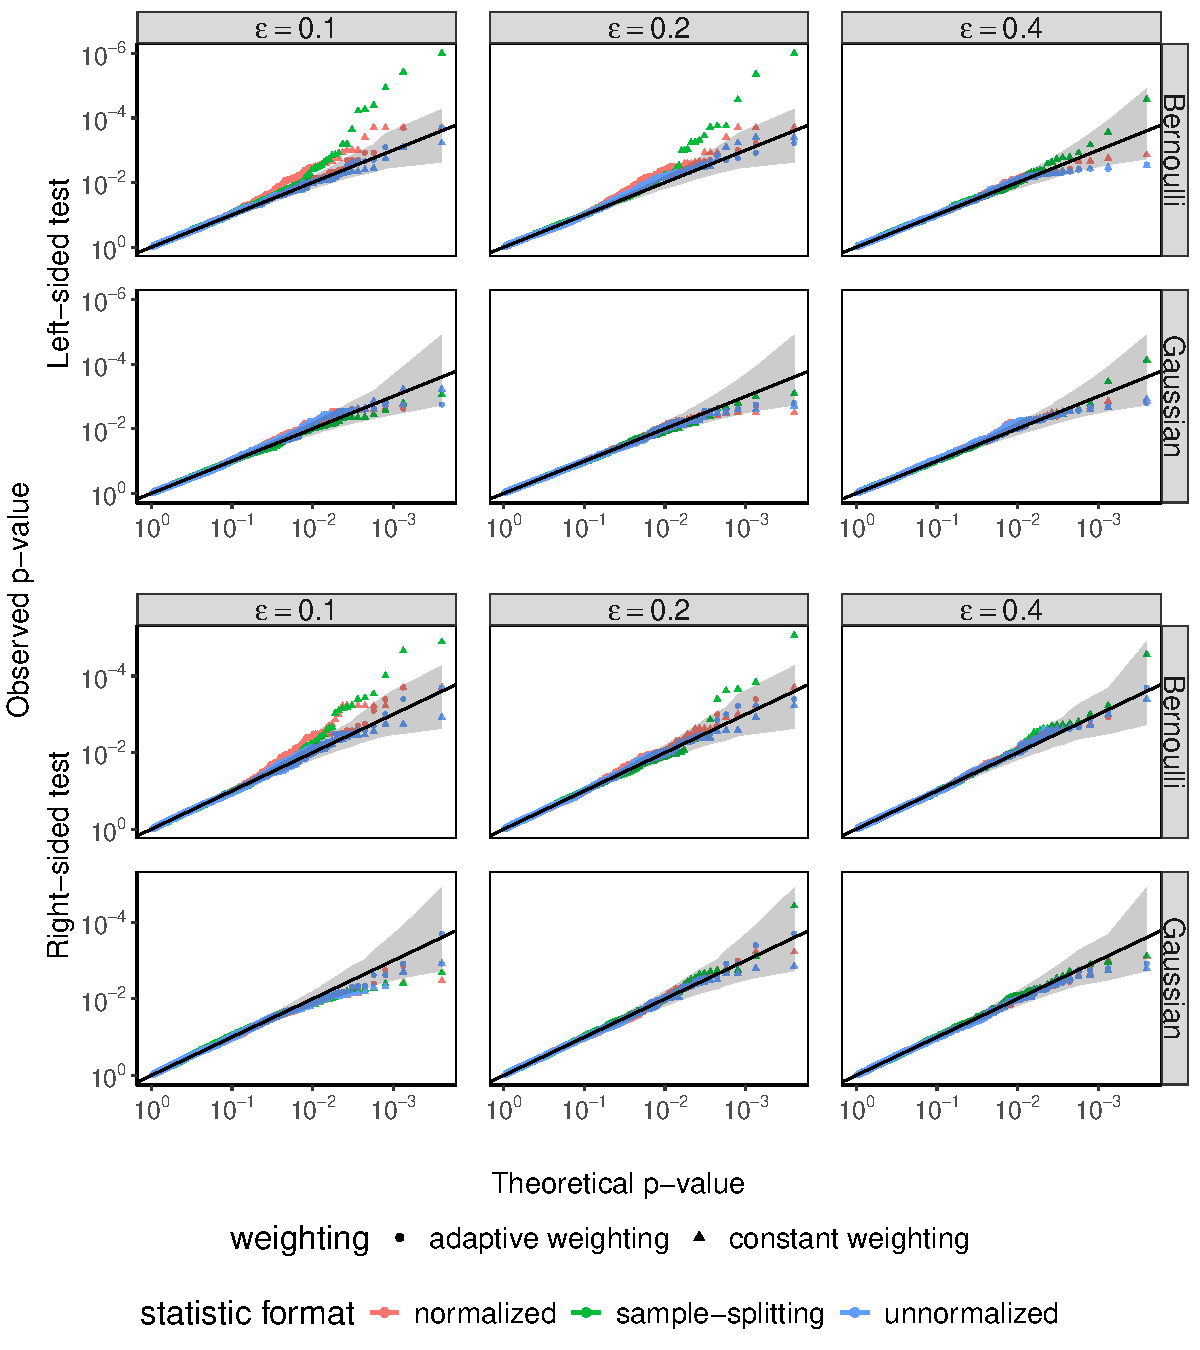
\includegraphics[width=0.93\textwidth]{figures-and-tables/simulation/eps_greedy_qq_plot.pdf}

	\caption{QQ-plot for the $5$ tests under different signal strength. The simulation is repeated for $2000$ times. The number of bootstrap used in each test is $5000$.}
	\label{fig:simulation-qq-plot-eps-greedy}
\end{figure}

\begin{figure}[!ht]
	\centering
	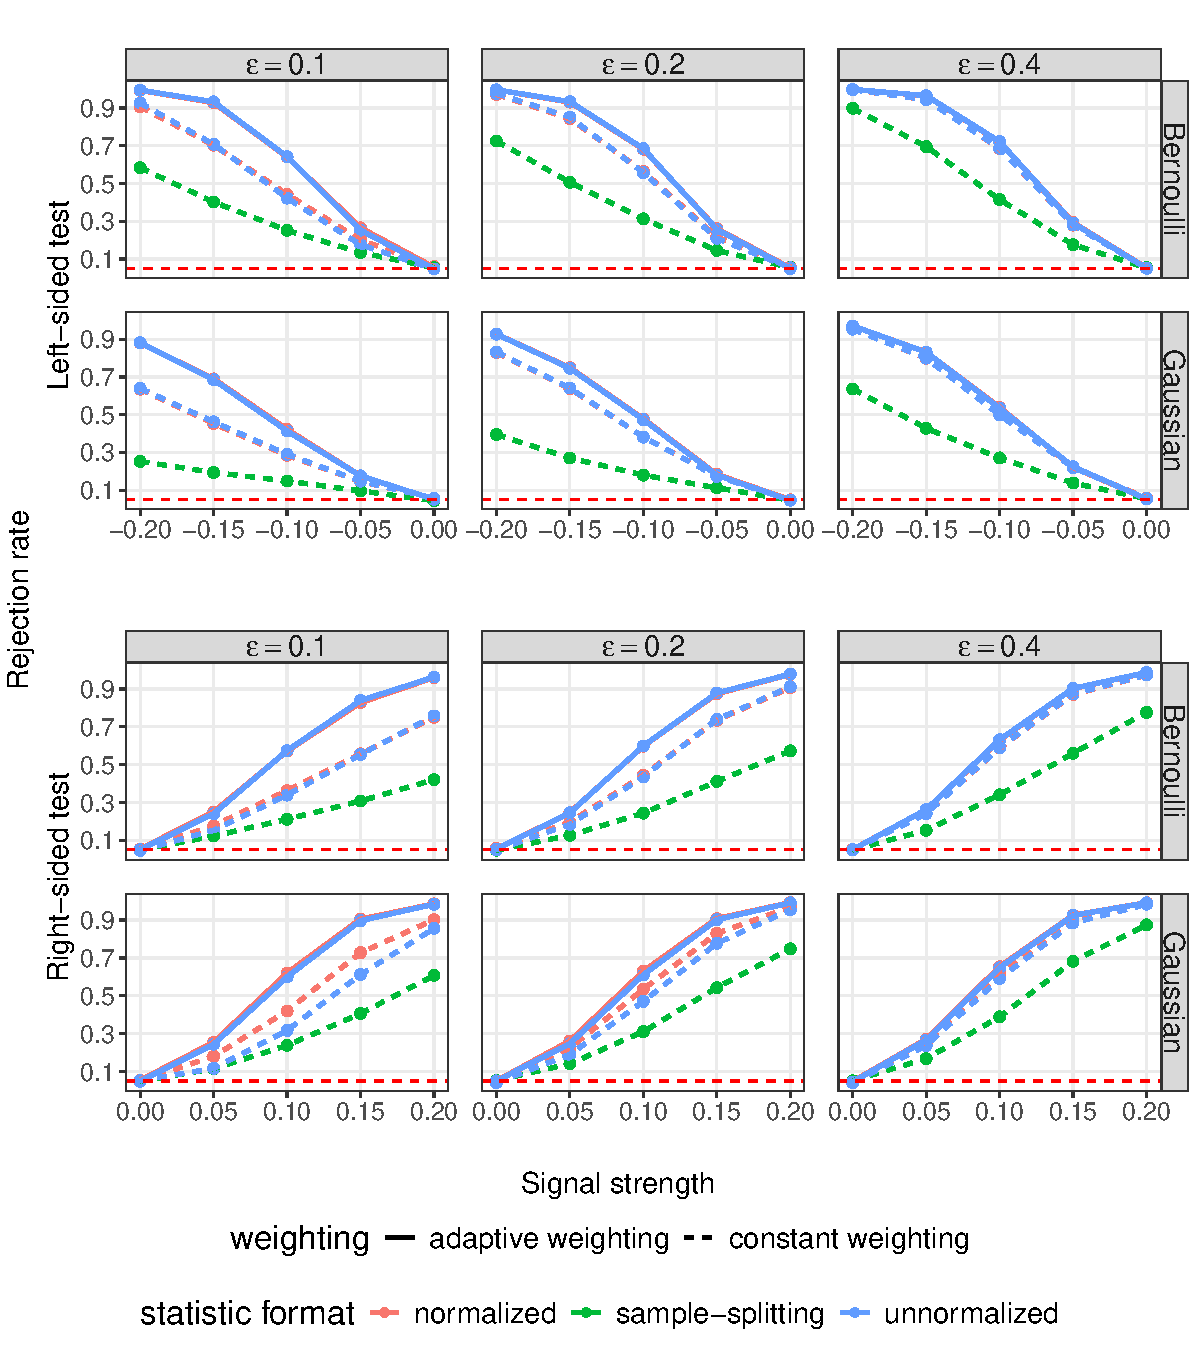
\includegraphics[width=0.93\textwidth]{figures-and-tables/simulation/eps_greedy_rejection_plot.pdf}

	\caption{Rejection rate for the $5$ tests under different signal strength. The simulation is repeated for $2000$ times. The number of bootstrap used in each test is $5000$.}
	\label{fig:simulation-rejection-plot-eps-greedy}
\end{figure}

\newpage 

\subsection{Power comparison: $m=1/2$ versus $m=1$}\label{sec:power-comparison}

We have observed from Figure \ref{fig:simulation-rejection-plot-thompson} that the adaptive weighting with $m=1/2$ is more powerful than the constant weighting ($m=0$). The natural question is then to ask which adaptive weighting scheme, $m=1$ or $m=1/2$, is better in terms of power. To investigate this question, we conduct a set of simulation with both unnormalized and normalized tests and the simulation invovles $4$ common distributions: Gaussian, Bernoulli, Poisson and Student distributions. We consider the Thompson sampling \eqref{eq:modified-cliped-TS} with $l_N=0.2$ and consider the sampel size $N=20,000$ and $N_1=N_2=10,000$. We set the significance level to be $0.05$. The distribution information can be summarized as below:
\begin{itemize}
	\item \textbf{Gaussian:} $Y_{u}(0)\sim N(\theta,1),Y_{u}(1)\sim N(0,0.25)$.
	\item \textbf{Bernoulli:} $Y_{u}(0)\sim\mathrm{Bern}(0.5+\theta),Y_{uN}(1)\sim\mathrm{Bern}(0.5)$.
	\item \textbf{Poisson:} $Y_{u}(0)\sim \mathrm{Pois}(1+\theta),Y_{u}(1)\sim \mathrm{Pois}(1)$.
	\item \textbf{Student:} $Y_{u}(0)\sim \theta+\mathrm{t}(4),Y_{u}(1)\sim \mathrm{t}(10)$ where $4$ and $10$ are degrees of freedom in the student distributions.
\end{itemize}
In particular, we choose $\theta\in\{0, 0.01, 0.02, 0.03,0.04\}$. The results are presented in Figure \ref{fig:power_comparison}. 

\paragraph{Implementation details.}

We center the outcome $Y_{uN}(s)$ by generating $\tilde Y_{uN}(s)=Y_{uN}(s)-\E[Y_{uN}(1)]$ and compare the test power for the average treatment effect $\E[\tilde Y_{uN}(0)]-\E[\tilde Y_{uN}(1)]$. The motivation for this operation is we do not want the test to be affected by the absolute signal strength. Asymptotically, such operation is equivalent to use $\WAIPW(s)$, defind as in~\eqref{eq:WAIPW}, when testing with the original data $(Y_{uN}(0),Y_{uN}(1))$. This is because the magnitude of $\theta$ is very small. Also, we want to point out that when $\E[\tilde Y_{uN}(s)]\sim 1/\sqrt{N}$ and $\E[\tilde Y_{uN}(1)]=0$ statistic $\WIPW(s)$ with $m=1$ is asymptotically equivalent to the sample mean, as proved in Lemma~\ref{lem:sample_mean_test_statistic}. In other words, the asymptotic power function for the sample mean test statistic is the same as the power function for the $m=1$ weighting when testing is performed on the transformed data $(\tilde Y_{uN}(0), \tilde Y_{uN}(1))$. 

\paragraph{Interpretation of the results.}


For all the other setups, it seems both $m=1$ and $m=1/2$ have very similar power performance. This means we would expect the sample mean test statistic should also have very comparable power performance with the weighting $m=1/2$. It is generally unclear if the test statistics considered in this paper are optimal or not under these distributions. As an exception, the sample mean test stiatistic has been shown to be near-optimal in some Gaussian setup, shown in Section 4.4 of \citet{Hirano2023}. 

\begin{figure}[!ht]
	\centering
	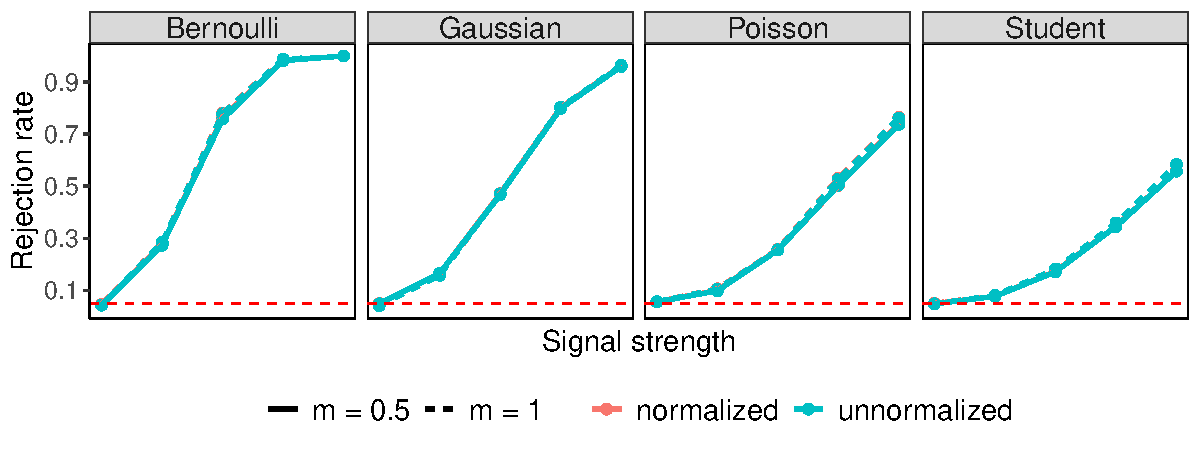
\includegraphics[width=0.99\textwidth]{figures-and-tables/simulation/rejection_plot_power_comparison.pdf}
	\caption{Rejection plots for adaptive weighting with $m=1$ and $m=1/2$ on the centered data $(\tilde Y_{uN}(0),\tilde Y_{uN}(1))$.}
	\label{fig:power_comparison}
\end{figure}

\clearpage

\section{Additional semi-synthetic data analysis results}\label{sec:additional_semi_synthetic}

We present additional results for the semi-synthetic data analysis in Section~\ref{sec:semi-sythetic-data}. Following the same procedure outlined in Section~\ref{sec:semi-sythetic-data}, we use $5000$ permuted sample to compute the $p$-values for the $5$ tests. The QQ-plot is shown in Figure \ref{fig:semi-synthetic-qq-plot}. We can see the message is similar to the one in Figure \ref{fig:simulation-qq-plot-eps-greedy} in Section~\ref{sec:semi-sythetic-data} when there is no signal.

\begin{figure}[!ht]
	\centering
	\begin{subfigure}{\textwidth}
		\centering
		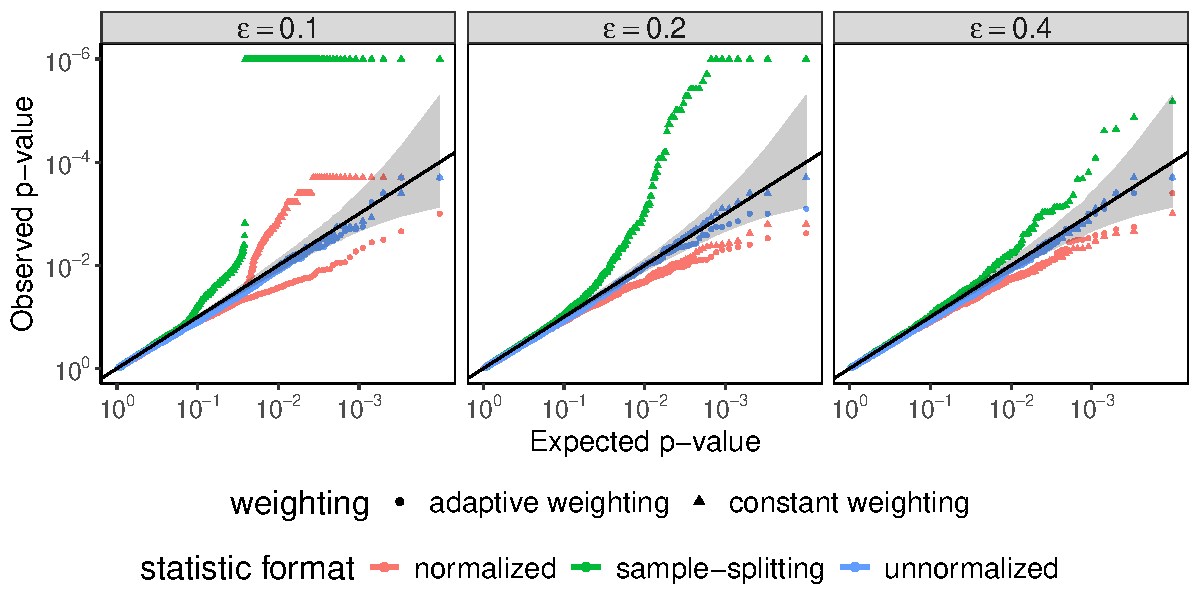
\includegraphics[width=0.95\textwidth]{figures-and-tables/realdata/qq_plot.pdf}
	\end{subfigure}
	\caption{QQ-plot for the semi-synthetic data analysis.}
	\label{fig:semi-synthetic-qq-plot}
\end{figure}


\end{document}






















 




